% Options for packages loaded elsewhere
\PassOptionsToPackage{unicode}{hyperref}
\PassOptionsToPackage{hyphens}{url}
\PassOptionsToPackage{dvipsnames,svgnames,x11names}{xcolor}
%
\documentclass[
  letterpaper,
  DIV=11,
  numbers=noendperiod]{scrartcl}

\usepackage{amsmath,amssymb}
\usepackage{iftex}
\ifPDFTeX
  \usepackage[T1]{fontenc}
  \usepackage[utf8]{inputenc}
  \usepackage{textcomp} % provide euro and other symbols
\else % if luatex or xetex
  \usepackage{unicode-math}
  \defaultfontfeatures{Scale=MatchLowercase}
  \defaultfontfeatures[\rmfamily]{Ligatures=TeX,Scale=1}
\fi
\usepackage{lmodern}
\ifPDFTeX\else  
    % xetex/luatex font selection
\fi
% Use upquote if available, for straight quotes in verbatim environments
\IfFileExists{upquote.sty}{\usepackage{upquote}}{}
\IfFileExists{microtype.sty}{% use microtype if available
  \usepackage[]{microtype}
  \UseMicrotypeSet[protrusion]{basicmath} % disable protrusion for tt fonts
}{}
\makeatletter
\@ifundefined{KOMAClassName}{% if non-KOMA class
  \IfFileExists{parskip.sty}{%
    \usepackage{parskip}
  }{% else
    \setlength{\parindent}{0pt}
    \setlength{\parskip}{6pt plus 2pt minus 1pt}}
}{% if KOMA class
  \KOMAoptions{parskip=half}}
\makeatother
\usepackage{xcolor}
\setlength{\emergencystretch}{3em} % prevent overfull lines
\setcounter{secnumdepth}{3}
% Make \paragraph and \subparagraph free-standing
\ifx\paragraph\undefined\else
  \let\oldparagraph\paragraph
  \renewcommand{\paragraph}[1]{\oldparagraph{#1}\mbox{}}
\fi
\ifx\subparagraph\undefined\else
  \let\oldsubparagraph\subparagraph
  \renewcommand{\subparagraph}[1]{\oldsubparagraph{#1}\mbox{}}
\fi


\providecommand{\tightlist}{%
  \setlength{\itemsep}{0pt}\setlength{\parskip}{0pt}}\usepackage{longtable,booktabs,array}
\usepackage{calc} % for calculating minipage widths
% Correct order of tables after \paragraph or \subparagraph
\usepackage{etoolbox}
\makeatletter
\patchcmd\longtable{\par}{\if@noskipsec\mbox{}\fi\par}{}{}
\makeatother
% Allow footnotes in longtable head/foot
\IfFileExists{footnotehyper.sty}{\usepackage{footnotehyper}}{\usepackage{footnote}}
\makesavenoteenv{longtable}
\usepackage{graphicx}
\makeatletter
\def\maxwidth{\ifdim\Gin@nat@width>\linewidth\linewidth\else\Gin@nat@width\fi}
\def\maxheight{\ifdim\Gin@nat@height>\textheight\textheight\else\Gin@nat@height\fi}
\makeatother
% Scale images if necessary, so that they will not overflow the page
% margins by default, and it is still possible to overwrite the defaults
% using explicit options in \includegraphics[width, height, ...]{}
\setkeys{Gin}{width=\maxwidth,height=\maxheight,keepaspectratio}
% Set default figure placement to htbp
\makeatletter
\def\fps@figure{htbp}
\makeatother
\newlength{\cslhangindent}
\setlength{\cslhangindent}{1.5em}
\newlength{\csllabelwidth}
\setlength{\csllabelwidth}{3em}
\newlength{\cslentryspacingunit} % times entry-spacing
\setlength{\cslentryspacingunit}{\parskip}
\newenvironment{CSLReferences}[2] % #1 hanging-ident, #2 entry spacing
 {% don't indent paragraphs
  \setlength{\parindent}{0pt}
  % turn on hanging indent if param 1 is 1
  \ifodd #1
  \let\oldpar\par
  \def\par{\hangindent=\cslhangindent\oldpar}
  \fi
  % set entry spacing
  \setlength{\parskip}{#2\cslentryspacingunit}
 }%
 {}
\usepackage{calc}
\newcommand{\CSLBlock}[1]{#1\hfill\break}
\newcommand{\CSLLeftMargin}[1]{\parbox[t]{\csllabelwidth}{#1}}
\newcommand{\CSLRightInline}[1]{\parbox[t]{\linewidth - \csllabelwidth}{#1}\break}
\newcommand{\CSLIndent}[1]{\hspace{\cslhangindent}#1}

\usepackage{booktabs}
\usepackage{longtable}
\usepackage{array}
\usepackage{multirow}
\usepackage{wrapfig}
\usepackage{float}
\usepackage{colortbl}
\usepackage{pdflscape}
\usepackage{tabu}
\usepackage{threeparttable}
\usepackage{threeparttablex}
\usepackage[normalem]{ulem}
\usepackage{makecell}
\usepackage{xcolor}
\usepackage{rotating}
\KOMAoption{captions}{tableheading}
\makeatletter
\makeatother
\makeatletter
\makeatother
\makeatletter
\@ifpackageloaded{caption}{}{\usepackage{caption}}
\AtBeginDocument{%
\ifdefined\contentsname
  \renewcommand*\contentsname{Table of contents}
\else
  \newcommand\contentsname{Table of contents}
\fi
\ifdefined\listfigurename
  \renewcommand*\listfigurename{List of Figures}
\else
  \newcommand\listfigurename{List of Figures}
\fi
\ifdefined\listtablename
  \renewcommand*\listtablename{List of Tables}
\else
  \newcommand\listtablename{List of Tables}
\fi
\ifdefined\figurename
  \renewcommand*\figurename{Figure}
\else
  \newcommand\figurename{Figure}
\fi
\ifdefined\tablename
  \renewcommand*\tablename{Table}
\else
  \newcommand\tablename{Table}
\fi
}
\@ifpackageloaded{float}{}{\usepackage{float}}
\floatstyle{ruled}
\@ifundefined{c@chapter}{\newfloat{codelisting}{h}{lop}}{\newfloat{codelisting}{h}{lop}[chapter]}
\floatname{codelisting}{Listing}
\newcommand*\listoflistings{\listof{codelisting}{List of Listings}}
\makeatother
\makeatletter
\@ifpackageloaded{caption}{}{\usepackage{caption}}
\@ifpackageloaded{subcaption}{}{\usepackage{subcaption}}
\makeatother
\makeatletter
\@ifpackageloaded{tcolorbox}{}{\usepackage[skins,breakable]{tcolorbox}}
\makeatother
\makeatletter
\@ifundefined{shadecolor}{\definecolor{shadecolor}{rgb}{.97, .97, .97}}
\makeatother
\makeatletter
\makeatother
\makeatletter
\makeatother
\ifLuaTeX
  \usepackage{selnolig}  % disable illegal ligatures
\fi
\IfFileExists{bookmark.sty}{\usepackage{bookmark}}{\usepackage{hyperref}}
\IfFileExists{xurl.sty}{\usepackage{xurl}}{} % add URL line breaks if available
\urlstyle{same} % disable monospaced font for URLs
\hypersetup{
  pdftitle={Investigating Extreme Linkage Topology in the Aerospace and Defence Industry},
  pdfauthor={ANON},
  colorlinks=true,
  linkcolor={blue},
  filecolor={Maroon},
  citecolor={Blue},
  urlcolor={Blue},
  pdfcreator={LaTeX via pandoc}}

\title{Investigating Extreme Linkage Topology in the Aerospace and
Defence Industry}
\author{ANON}
\date{}

\begin{document}
\maketitle
\ifdefined\Shaded\renewenvironment{Shaded}{\begin{tcolorbox}[sharp corners, interior hidden, enhanced, borderline west={3pt}{0pt}{shadecolor}, frame hidden, boxrule=0pt, breakable]}{\end{tcolorbox}}\fi

\hypertarget{abstract}{%
\subsection*{Abstract}\label{abstract}}
\addcontentsline{toc}{subsection}{Abstract}

This paper analyses return and volatility spillovers among 21 global
aerospace and defence (A\&D) companies from six countries and three
continents using quantile-based models and daily data from August 23,
2010, to July 1, 2022. The results show that both return and volatility
spillovers vary over time, and those estimated at normal market
conditions, intensify during COVID-19 and Russia-Ukraine war periods.
Spillovers of returns estimated at lower and upper quantiles exceed
those estimated at the middle quantile. Volatility spillover is
extremely high at the upper quantile and exhibits low variability.
Chinese defence stocks are segmented from the rest under normal return
conditions and a moderate volatility state. In contrast, they are
somewhat integrated under extreme return conditions and volatility
states. Hence, Chinese defence stocks entail more diversification
benefits under normal conditions than in bear or bull markets. Further
analysis shows that geopolitical risk consistently plays a significant
role in driving both returns and volatility spillovers, especially
during the pandemic and war periods, without ignoring the role of
macroeconomic and financial variables. These results have implications
for investors concerned with stock portfolio management under various
return and volatility conditions and for policymakers preoccupied with
policy design under unstable periods

\textbf{keywords:} Aerospace and defence companies; Ukrainian war;
Russia; quantile vector-autoregression (QVAR); COVID-19.

\textbf{JEL codes:} C32, G15.

\hypertarget{introduction}{%
\section{Introduction}\label{introduction}}

On 24 February 2022, Russia invaded Ukraine, instigating a brutal war
that has led to wide-scale devastation and the consequences of which
will be felt far into the future. While the humanitarian effects are
almost incomprehensible, this war has substantially affected the global
economy, financial markets, commodity markets (notably energy and grain
prices), and the fortunes of defence companies. There appears to be no
end to the war, and spending on defence has experienced a notable
increase globally, with global military expenditure surpassing US\$ 2.2
trillion for the first time in 2022. During that year, the United States
(U.S.) had the highest military spending, with a total of US\$ 877
billion, followed by China with US\$ 292 billion, Russia with US\$ 86.0
billion, India with US\$ 81.0 billion, Saudi Arabia with US\$ 75.0
billion, the United Kingdom (U.K.) with US\$ 69.0 billion, Germany with
US\$ 56.0 billion, and France with US\$ 54.0 billion.\footnote{Data are
  according to Stockholm International Peace Research Institute
  (\url{https://sipri.org/})}

This increase in defence spending has led to the global aerospace and
defence (A\&D) industry outperforming equity markets in terms of return.
According to Refinitiv Eikon, on January 2022 the total return of the
A\&D industry equated to 13.89\% YoY, compared to -3.45\% YoY for global
equity markets. This occurred even though the average total market
capitalisation of A\&D companies represents only 1\% of worldwide equity
markets. Furthermore, Refinitiv Eikon reported total revenues for 2022
were \$US 665 billion YoY for the A\&D sector, with the top 21 largest
companies (according to revenue) capturing 75\% of this total revenue
(See Appendix Table~\ref{tbl-A1} for detailed Market Analysis). Merger
and acquisition activity in the A\&D industry was also high, with 361
deals amounting to a total value, including net debt, of \$US 36
billion\footnote{All market analysis was conducted using Refinitiv Eikon
  on February 22, 2023. The A\&D sample consisted of 351 publicly listed
  securities with a total market capitalization of US\$ 1.37 trillion.
  The global equity market capitalisation at this time was US\$ 118
  trillion.}. Given the ongoing war and its effects, along with the
recent market performance of many A\&D companies, our study investigates
the network topology of the return and volatility spillovers among major
companies from the global A\&D industry and the factors that drive these
spillovers. Using a quantile-based approach to spillovers, we explicitly
consider the transmission pathway of return and volatility from one
company to another under various market return conditions and volatility
states. Furthermore, we conduct multiple regressions to understand the
role of geopolitical risk in driving return and volatility spillovers
while considering various macroeconomic and financial variables.

Related literature on this topic remains relatively scarce, which is
unsurprising given this is an ongoing conflict. Studies analyzing the
A\&D industry date back at least as far as the 1960s, mainly focusing on
the investment quality of companies operating in this industry (Butler
Jr, 1966b, 1966a, 1967) and their profits and market performance (Agapos
and Gallaway, 1970; Suarez, 1976; Bohi, 1973). McDonald and Kendall
(2011) study the effects of war on the U.S. defence industry, focusing
on 16 firms that provided military equipment to the Department of
Defence. Applying a cumulative prediction error (CPE) technique, they
find that stock prices of defence firms tend to increase because of
military actions. Capelle-Blancard and Couderc (2008) analyse the effect
of media information on defence companies only, showing that news
relating to earnings announcements and analyst recommendations are
significant in explaining abnormal returns for these companies.
Recently, Federle et al.~(2022) analyse stock market responses to the
war in Ukraine, finding that firms closer to Ukraine suffered from a
relative proximity penalty, experiencing negative equity returns during
the four weeks surrounding the beginning of the war. Le et al.~(2023)
use war-related news articles to investigate the market response of some
companies to the war in Ukraine, showing a negative impact on airline
stocks and a positive impact on defence stocks. Zhang et al.~(2022)
consider the co-movements between geopolitical risk and the returns and
volatility of global aerospace and defence companies, indicating
significant co-movements around the onset of the war in Ukraine. This is
labelled a `flight-to-arms' phenomenon, with co-movement found to be
significant for many European and U.S. companies in the sample.

This paper contributes to the above body of literature by analysing the
network of returns and volatility spillovers across major A\&D companies
using a quantile-based connectedness method and analyzing drivers of
spillovers. First, the flexibility of this connectedness approach
enables us to account for various market return conditions and
volatility states. This is an important feature as previous findings
highlight the importance of considering the sign of return shocks and
size of volatility shocks when studying the spillover effects in
financial markets (see, Bouri et al., 2020; Chatziantoniou et al., 2021;
iq et al., 2021; Iqbal et al., 2022). This should add to Zhang et
al.~(2022) and Le et al.~(2023), that consider only mean-based models.
Second, our sample of 21 A\&D companies incorporates eight out of the
ten most significant in the world by revenue and covers six countries,
namely the U.S., the U.K., France, Germany, China and Singapore, across
three continents (North America, Europe, and Asia) over the period
August 23, 2010 to July 1, 2022. The sample period covers events such as
the Russian invasion of Crimea in 2014, the COVID-19 pandemic of 2020,
and the onset of the Russia-Ukraine war in 2022, thus enabling the
identification of significant spillovers across a varying set of global
turbulent market conditions and geopolitical events. Third, analysing
the factors driving the return and volatility spillovers across various
market conditions constitutes another contribution to the literature on
A\&D companies (Federle et al., 2022; Le et al., 2023; Zhang et al.,
2022). Specifically, it illustrates the importance of geopolitical risk
in increasing the spillover effect of both returns and volatility while
accounting for the significance of macroeconomic and financial
variables.

The main results show intensified spillover effects for stock returns
and volatility under extreme market conditions and evidence of time
evolution in spillovers, particularly for lower and upper tails returns.
This suggests that the system of spillovers under extreme market
conditions, irrespective of whether it is a bull or bear market, is
unstable. Thus, it should be carefully monitored, given its potential
consequences on portfolio and risk management in the A\&D industry. An
additional analysis analysing the drivers of spillovers with multiple
regressions shows the impact of heightened geopolitical risk around the
Russian-Ukraine war period on the return and volatility spillovers
across A\&D companies in most of the quantiles considered. Furthermore,
the level of returns and volatility spillovers is also driven by
macroeconomic and financial variables such as corporate credit
conditions, stock market volatility, short-term liquidity risk, and
real-time US business conditions ( measured using the Aruoba et al.,
2009 methodology). Therefore, participants in the A\&D industry,
especially in the U.S. and Europe, should closely monitor the global
geopolitical environment given its significant impact on the dynamics of
information transmission in the A\&D industry and, thus, the integration
of A\&D stocks and possibilities of diversification. The findings also
highlight the tail risk propagation within the network system of
aerospace and defence stocks, which should concern risk managers and
policymakers.

The paper proceeds as follows. Section 2 describes the dataset. Section
3 provides a quantile-based spillover approach. Section 4 presents and
discusses the results. Section 5 concludes.

\hypertarget{data}{%
\section{Data}\label{data}}

Our dataset comprises daily closing prices of 21 global aerospace and
defence companies in six countries (U.S., U.K., France, Germany, China,
Singapore) across three continents (North America, Europe, and Asia)
from August 23, 2010 to July 1, 2022. The selected companies are chosen
to be large and liquid, with an individual market capitalisation
exceeding US\$ 8 Billion. The list of companies is provided in Appendix
Table~\ref{tbl-A1}. According to the Refinitiv, our sample captures 72\%
of the total market capitalisation of the global A\&D
industry\footnote{At the time of writing, the Refinitiv Eikon database
  valued the market capitalisation of the Aerospace and Defence industry
  at \$US1.37 trillion.}. The sample period is selected according to the
availability of A\&D stock price data from Refinitiv, especially for the
Chinese Aecc Aviation Power `A' because it exhibited many zero price
fluctuations before the start of the sample period.

Appendix Figure A1 plots the price series and highlights the country of
incorporation. Furthermore, Appendix Figure A2 and Figure A3 display the
log-return and volatility\footnote{Daily volatility is calculated as the
  squared of daily log-returns (Zhang et al., 2022).} series,
respectively. The price series reveal several distinct groupings in
their movements. For many cases, prices in Figure A1 show common
movement with a regime shift towards higher prices and more considerable
volatility around 2020. Notably, Chinese stocks experienced a shock in
2016 of a similar magnitude to that of 2020. In July 2016, it was
reported that China had performed a week of military drills in the South
China Sea amid legal debates regarding its territorial claims to
regional areas, which could account for this increase in volatility. In
Figure A2, there is a large variability in the returns that coincides
with the peak of COVID-19 in 2020 and the onset of the Russia-Ukraine
war in early 2022, especially for most U.S.-European A\&D stocks. Based
on Figure A3, it is clear that the volatility of some A\&D companies,
such as Boeing, Transdigm, Safran, and Rolls-Royce Holdings experienced
a spike around the pandemic outbreak and the beginning of the
Russia-Ukraine war.

Appendix Figure A2 plots the price series levels and highlights the
country of incorporation. Furthermore, Appendix Figure A3 and Figure A4
display the log-return and volatility series, respectively. The price
series levels reveal several distinct groupings in their movements. For
many cases, price series levels in Figure A2 show common movement with a
regime shift towards higher prices and larger volatility around 2020.
Notably, Chinese stocks experienced a shock in 2016 of a similar
magnitude to that of 2020. In July 2016, it was reported that China had
performed a week of military drills in the South China Sea amid legal
debates regarding its territorial claims to regional areas, which could
account for this increase in volatility. In Figure A3, we notice a large
variability in the returns around the peak of COVID-19 in 2020 and the
Russia-Ukraine war in early 2022, especially for most US-European A\&D
stocks. Based on Figure A4, we observe that the volatility of some A\&D
companies such as Boeing, Transdigm, Safran, and Rolls-Royce Holdings
experienced a spike around the pandemic outbreak and the Russia-Ukraine
war.

Appendix Table~\ref{tbl-A2} and Table~\ref{tbl-A3} present summary
statistics for daily returns and volatility series. Notably, Table 7
illustrates that the distributions of the daily returns series are
mostly skewed to the left and exhibit fat ``tailedness'', with Airbus,
Boeing, Rolls-Royce Holdings, Safran, and Transdigm experiencing the
highest daily standard deviations. These companies are either directly
in the aviation industry or supply to it. For example, Rolls-Royce
supplies the Trent engine to Airbus. In this regard, airlines were hit
particularly hard during the COVID-19 pandemic, with an estimated
economic loss of US\$168 billion in 2020 (Bouwer et al. 2022), which may
be a factor in the observed volatility. All return series are
stationary, as shown by the Augmented Dickey-Fuller (ADF) and
Phillips-Perron (PP) test statistics. The same is true for the
volatility series, as reported in Appendix Table~\ref{tbl-A3}

Furthermore, we consider extreme volatility events, which coincide with
the peak of the COVID-19 pandemic outbreak and indicate in Table 1 that
the most volatile A\&D stock is Rolls Royce Holdings. The company
reported a loss of £4 billion for 2020, which led to a need to raise
£7.3 billion in debt and equity and cut almost one-fifth of its
workforce (Sillars 2021). Unsurprisingly, Table~\ref{tbl-Xtremes}
indicates that the five highest daily volatility scores mainly occur
around the end of March 2020 at the height of the uncertainty during the
onset of the COVID-19 pandemic.

\hypertarget{tbl-Xtremes}{}
\begin{table}[H]
\caption{\label{tbl-Xtremes}Extremely votality events }\tabularnewline

\centering
\begin{tabular}[t]{llrrl}
\toprule
Date & stock & return & volatility & country\\
\midrule
2020-03-18 & Airbus & -0.25 & 0.06 & France\\
2020-03-16 & Boeing & -0.27 & 0.07 & US\\
2020-11-09 & Rolls-Royce Holdings & 0.36 & 0.13 & UK\\
2020-03-18 & Safran & -0.26 & 0.07 & France\\
2020-03-18 & Transdigm Group & -0.25 & 0.06 & US\\
\bottomrule
\end{tabular}
\end{table}

\hypertarget{methodology}{%
\section{Methodology}\label{methodology}}

The nature and strength of spillovers across financial markets have
traditionally been measured using conventional mean estimators such as
the connectedness approach of Diebold and Yılmaz (2014). Interestingly,
Tomohiro Ando, Greenwood-Nimmo, and Shin (2022) argue that systemic
shocks are likely to be much larger than average shocks and that extreme
negative return (or low volatility) shocks do not necessarily propagate
in the same way as extreme positive return (or high volatility) shocks.
Therefore, quantile-based estimators allow for identifying whether the
spillover effects' topology changes with the shock distribution's size
and sign as captured by the various quantiles of the shock distribution
(Bouri et al. 2020a).

To study the return and volatility connectedness across 21 global
aerospace and defence companies, we use the quantile-VAR-based
connectedness approach following Ando et al.~(2022)\footnote{Existing
  studies in the Deibold-Yilmaz network literature use windows ranging
  from 100-250 days. Sensitivity analysis has been done and available
  upon request.}. This approach extends the mean-based connectedness
approach of Diebold and Yılmaz (2014) and thus allows for capturing the
extreme connectedness estimated at the lower, middle, and upper
quantiles. For returns, this helps obtain the connectedness of return
shocks in bear, normal, and bull markets. For volatility, it helps
capture the connectedness of volatility shocks in low, middle, and high
volatility states.

We consider a portfolio enivroment, where stocks are indexed
i=1,2,\ldots,N, and time periods are indexed t=1,2,\ldots,T. Based on a
quantile regression (Koenker, 2005), we consider a quantile-VAR process
of p\textsuperscript{th} order for a set of N return (volatility) series
for time T, \(y_{it}=\{y_{t=1,i=1},\dots,y_{t=T,i=N}\}\) , as given by:

\begin{equation}\protect\hypertarget{eq-one}{}{
y_{t}=c_{i(\tau)}+\sum_{j=1}^{p} B_{j,(\tau)} y_{t-j}+e_{t(\tau)}, t=1,\dots,T
}\label{eq-one}\end{equation}

where, \(c_{(\tau)}\) denotes a vector of constant terms at quantile
\(\tau\), \(B_{j(\tau)}\) represents the matrix of the
j\textsuperscript{th} lagged coefficients of the dependent variable at
quantile \(\tau\), with i =1,\ldots, p, and \(e_{t(\tau)}\) denotes a
vector of error terms at quantile \(\tau\). Equation~\ref{eq-one} is
estimated by assuming that the error terms conform to the population
quantile restriction, \(Q_t(e_{t(\tau)} |y_{t=1},\dots,y_{t=p})=0\) .

We express the \(\tau^{th}\) conditional quantile of response y as:

\begin{equation}\protect\hypertarget{eq-two}{}{
Q_t(y_t |y_{t=1},\dots,y_{t=p})=c_{(\tau)}+\hat{B_{i(\tau)}} y_{t-i}
}\label{eq-two}\end{equation}

Following the approach of Diebold and Yılmaz (2014) , we compute return
and volatility connectedness measures based on a quantile variance
decomposition.

We represent Equation~\ref{eq-two} as an infinite order vector moving
average process:

\begin{equation}\protect\hypertarget{eq-three}{}{
y_t=\mu_{(\tau)}+\sum_{s=0}^{\infty}A_{s(\tau)}e_{t-s(\tau)}, t=1,\dots.T
}\label{eq-three}\end{equation}

where,

\begin{align*}
\mu{(\tau)}= \frac{c_{\tau}}{\left (I_n-B_{1(\tau)}-\dots-B_{p(\tau)} \right)} \\
A_{s(\tau)}= \begin{cases} 0, s<0 \\ I_n, s=0 \\ B_{1(\tau)}A_{s-1(\tau)}+\dots+B_{p(\tau)}A_{s-p(\tau)}, s>0 \end{cases} \\
\text{and $y_t$ is given by the sum of $e_{t(\tau)}$}
\end{align*}

The generalized forecast error variance decomposition
(GFEVD),\(\theta^h_{i,j}\), is computed as in Diebold and Yılmaz (2014).
The GFEVD reflects the contribution of the i\textsuperscript{th} stock
return (volatility) to the variance of the forecast error of the stock
return (volatility) i\textsuperscript{th} at h-steps ahead and is
defined as:

\begin{equation}\protect\hypertarget{eq-four}{}{
\theta^{(h)}_{j \leftarrow i,(\tau)}= \frac{\sigma_{ii}^{-1}\sum_{l=0}^{h}(e_j^{'}h_h \Omega_{(\tau)} e_j)^2}{\sum_{h=0}^{H-1}(e_i^{'}h_h \Omega_{(\tau)} e_i)}
}\label{eq-four}\end{equation}

where, V is the variance matrix of the vector of residuals,
\(\sigma_{ii}\) is the j\textsuperscript{th} diagonal element of the V
matrix, and \(e_i\)denotes a vector with a value of 1 for the
i\textsuperscript{th} element and 0 otherwise.

Its scaled version,\(\theta_{j\leftarrow i,(\tau)}^h\) , is represented
as:

\begin{equation}\protect\hypertarget{eq-five}{}{
\theta_{j\leftarrow i,(\tau)}^h=\frac{\theta^{(h)}_{j \leftarrow i,(\tau)}}{\sum_{j=1}^N \theta^{(h)}_{j \leftarrow i,(\tau)}}
}\label{eq-five}\end{equation}

The scaled version measures the spillover of the idiosyncratic shock
affecting variable i onto variable j (Tomohiro Ando, Greenwood-Nimmo,
and Shin 2022).

Various spillover measures are estimated at each quantile and are
summarised in Table 2. The third column, ``Description'', describes how
these can be interpreted in terms of the system of spillovers. Note
that, by construction, own share and FROM sum to one for i=1,2,..,m;
however, TO can take values bigger than or less than one.

The lag order of the quantile VARs is selected based on SIC. It equals 1
for the quantile-VAR of the return series and 2 for the quantile-VAR of
the volatility series. As for the forecast horizon (H), we use ten days.
Furthermore, we conduct a time-varying spillover analysis (Diebold \&
Yilmaz, 2014) based on a rolling window of 200 days. To assess the
robustness of our results, we use a fixed window length of 200 days and
a 5-step forecast horizon and show that our spillover results remain
almost the same, suggesting their robustness to the window size and
forecast horizon. These results are not reported here but are available
on request from the authors.

\begin{longtable}[]{@{}
  >{\raggedright\arraybackslash}p{(\columnwidth - 4\tabcolsep) * \real{0.2639}}
  >{\raggedright\arraybackslash}p{(\columnwidth - 4\tabcolsep) * \real{0.4167}}
  >{\raggedright\arraybackslash}p{(\columnwidth - 4\tabcolsep) * \real{0.3194}}@{}}
\caption{Description of modelling outputs}\tabularnewline
\toprule\noalign{}
\begin{minipage}[b]{\linewidth}\raggedright
Name
\end{minipage} & \begin{minipage}[b]{\linewidth}\raggedright
Formula
\end{minipage} & \begin{minipage}[b]{\linewidth}\raggedright
Description
\end{minipage} \\
\midrule\noalign{}
\endfirsthead
\toprule\noalign{}
\begin{minipage}[b]{\linewidth}\raggedright
Name
\end{minipage} & \begin{minipage}[b]{\linewidth}\raggedright
Formula
\end{minipage} & \begin{minipage}[b]{\linewidth}\raggedright
Description
\end{minipage} \\
\midrule\noalign{}
\endhead
\bottomrule\noalign{}
\endlastfoot
Own share &
\(                                                                                                                                                                                                                                                                                                                                                                                                                                                                                                                                                                                                                                                                                                                                                                                                                                                                                                                                                                                                                                                                                                                                                                                                                                                                                                                                                                                                                                                                
                                                                                                                                                                                                                                                                                                                                                                                                                                                                                                                                                                                                                                                                                                                                                                                                                                                                                                                                                                                                                                                                                                                                                                                                                      \tilde{\theta_{j\leftarrow i,(\tau)}^h}                                                                                                                                                                                                                   
                                                                                                                                                                                                                                                                                                                                                                                                                                                                                                                                                                                                                                                                                                                                                                                                                                                                                                                                                                                                                                                                                                                                                                                                                      \)
& The proportion of the h-steps-ahead GFECD of the ith variable that can
be attributed to the shocks to variable i \\
FROM &
\(                                                                                                                                                                                                                                                                                                                                                                                                                                                                                                                                                                                                                                                                                                                                                                                                                                                                                                                                                                                                                                                                                                                                                                                                                                                                                                                                                                                                                                                                
                                                                                                                                                                                                                                                                                                                                                                                                                                                                                                                                                                                                                                                                                                                                                                                                                                                                                                                                                                                                                                                                                                                                                                                                                      F_{i \leftarrow \cdot,(\tau)}^h =\sum_{j=1,i \ne j}^m \theta_{j\leftarrow i,(\tau)}^h                                                                                                                                                                     
                                                                                                                                                                                                                                                                                                                                                                                                                                                                                                                                                                                                                                                                                                                                                                                                                                                                                                                                                                                                                                                                                                                                                                                                                      \)
& Measures the total spillover from the system to i, capturing external
condition effects on i. \\
TO &
\(                                                                                                                                                                                                                                                                                                                                                                                                                                                                                                                                                                                                                                                                                                                                                                                                                                                                                                                                                                                                                                                                                                                                                                                                                                                                                                                                                                                                                                                                
                                                                                                                                                                                                                                                                                                                                                                                                                                                                                                                                                                                                                                                                                                                                                                                                                                                                                                                                                                                                                                                                                                                                                                                                                      T_{\cdot \leftarrow i,(\tau)}^h =\sum_{j=1,i \ne j}^m \theta_{j\leftarrow i,(\tau)}^h                                                                                                                                                                     
                                                                                                                                                                                                                                                                                                                                                                                                                                                                                                                                                                                                                                                                                                                                                                                                                                                                                                                                                                                                                                                                                                                                                                                                                      \)
& Measures the total spillover from i to the system, capturing the
influence of ith node in the network. \\
NET &
\(                                                                                                                                                                                                                                                                                                                                                                                                                                                                                                                                                                                                                                                                                                                                                                                                                                                                                                                                                                                                                                                                                                                                                                                                                                                                                                                                                                                                                                                                
                                                                                                                                                                                                                                                                                                                                                                                                                                                                                                                                                                                                                                                                                                                                                                                                                                                                                                                                                                                                                                                                                                                                                                                                                      T_{\cdot \leftarrow i,(\tau)}^h -F_{i \leftarrow \cdot,(\tau)}^h                                                                                                                                                                                          
                                                                                                                                                                                                                                                                                                                                                                                                                                                                                                                                                                                                                                                                                                                                                                                                                                                                                                                                                                                                                                                                                                                                                                                                                      \)
& Meaures the directional connectedness of variable i. \\
TOTAL &
\(                                                                                                                                                                                                                                                                                                                                                                                                                                                                                                                                                                                                                                                                                                                                                                                                                                                                                                                                                                                                                                                                                                                                                                                                                                                                                                                                                                                                                                                                
                                                                                                                                                                                                                                                                                                                                                                                                                                                                                                                                                                                                                                                                                                                                                                                                                                                                                                                                                                                                                                                                                                                                                                                                                      S_{\tau}^h=m^{-1}\sum                                                                                                                                                                                                                                     
                                                                                                                                                                                                                                                                                                                                                                                                                                                                                                                                                                                                                                                                                                                                                                                                                                                                                                                                                                                                                                                                                                                                                                                                                      F_{i \leftarrow \cdot,(\tau)}^h                                                                                                                                                                                                                           
                                                                                                                                                                                                                                                                                                                                                                                                                                                                                                                                                                                                                                                                                                                                                                                                                                                                                                                                                                                                                                                                                                                                                                                                                      \)
& Is the sum of the from system estimates. \\
\end{longtable}

\hypertarget{results}{%
\section{Results}\label{results}}

In the context of global defence stocks, we are primarily interested in
the spillover effects due to crisis periods and conflict events,
particularly relevant in the current geopolitical climate. Regarding
financial risk management, the propagation of idiosyncratic risk
contagion is often defined as the difference in how the shock propagates
during extreme events relative to normal times (Londono 2019). Our
analysis thus attempts to investigate how much of the uncertainty
associated with A\&D stocks can be attributed to the idiosyncratic
shocks coming from these stocks as the shock size varies.

We present the return and volatility spillovers across the 21 A\&D
stocks under study. The sample period of August 23, 2010 - July 1, 2022,
covers normal and extreme market conditions, including the COVID-19
outbreak and the Russia-Ukraine war.

\hypertarget{network-topology-of-return-and-volatility-spillovers}{%
\subsection{Network topology of return and volatility
spillovers}\label{network-topology-of-return-and-volatility-spillovers}}

To understand the aggregate spillover intensity among A\&D stocks, we
visualise the results of a full-sample analysis for both returns and
volatility at the median, 5th and 95th percentile. The network
visualisation reflects the strength of the bilateral spillovers by the
relative thickness of the edges. At the same time, the size of each node
is proportional to the square root of the total spillover (inwards and
outwards) (Tomohiro Ando, Greenwood-Nimmo, and Shin 2022). Furthermore,
the country of origin of the company is represented by colour.

\hypertarget{return-spillovers}{%
\subsubsection{Return spillovers}\label{return-spillovers}}

Figure~\ref{fig-rtn} illustrates the network visualisation of the
bilateral spillover effects of the 21 return series, whereas
Figure~\ref{fig-vol} displays the exact visualisation for the 21
volatility series. Some similar patterns emerge, notably the consistent
size of all stock nodes representing the significant aggregate spillover
effects in both directions for median and extreme upper quantiles.
However, there are also some crucial differences. Firstly, the most
substantial individual pairwise spillover effects are observed at the
median conditional distribution, primarily within countries. Notably,
Chinese stocks show the most robust linkages within the country but the
weakest linkages outside their country of origin. This corresponds to
literature relating to general stock market trends observed in China;
for example, Valukonis (2014) finds that following the recovery from the
financial crisis of 2008, Chinese and US stock market indices display a
weak correlation which is perhaps due to Chinese markets being somewhat
isolated from global markets and not as influenced by globalisation as
other markets may be.

In contrast, all pairwise spillover effects are weaker at the extremes
of the return distribution. This finding is consistent with previous
studies, which show that in times of stress, the network is
characterised by a more significant number of weaker bilateral linkages
increasing the weight completeness of the network (Dungey et al., 2019;
Ando et al., 2022). In our context, this would mean that while shock
spillovers between individual stock pairs are small, the overall
connectedness of the system is increasing in extreme bull (the extreme
upper quantile illustrated by Figure~\ref{fig-rtn95}) and bear (the
extreme lower quantile illustrated by Figure~\ref{fig-rtn5}) markets,
meaning that the shock propagation is higher under extreme return
conditions. Furthermore, unlike bull market conditions, aggregate
spillover effects (represented by node size) are smaller in bear market
conditions, although US stock have more influence than countries.

\begin{figure}[H]

\begin{minipage}[t]{0.50\linewidth}

{\centering 

\raisebox{-\height}{

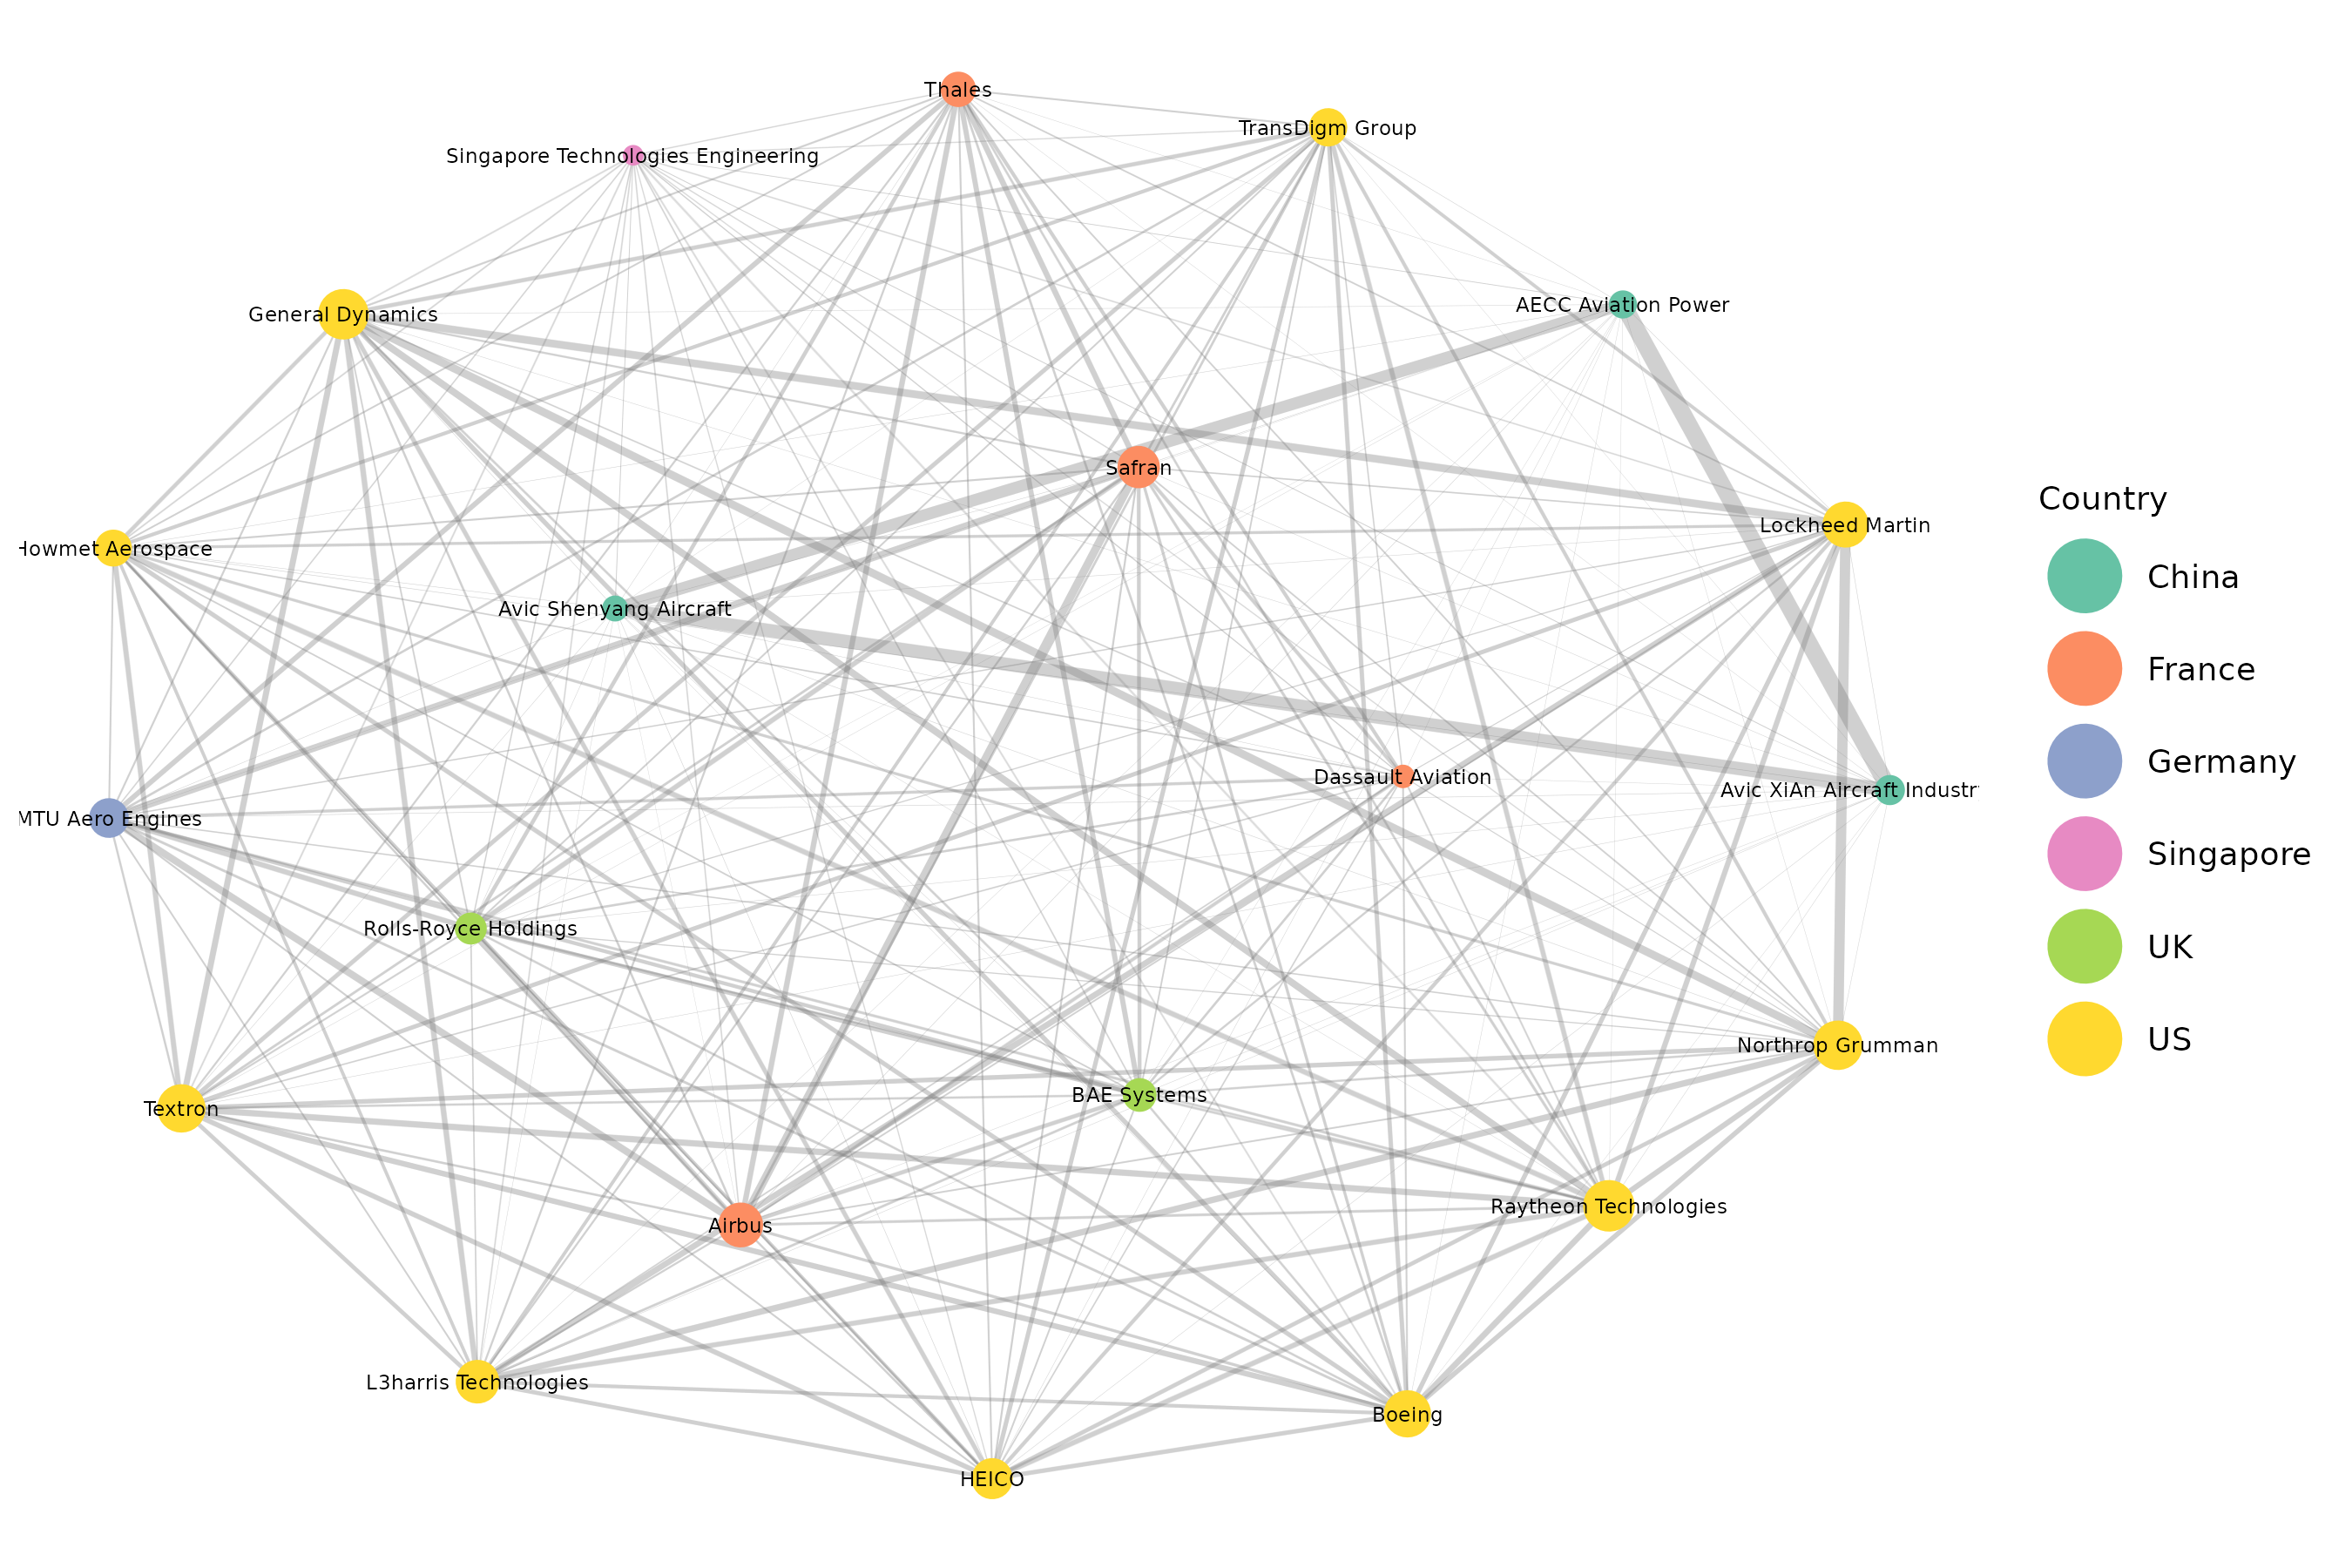
\includegraphics{plots/fig-rtn50.png}

}

}

\subcaption{\label{fig-rtn50}Middle quantile (50th Percentile)}
\end{minipage}%
%
\begin{minipage}[t]{0.50\linewidth}

{\centering 

\raisebox{-\height}{

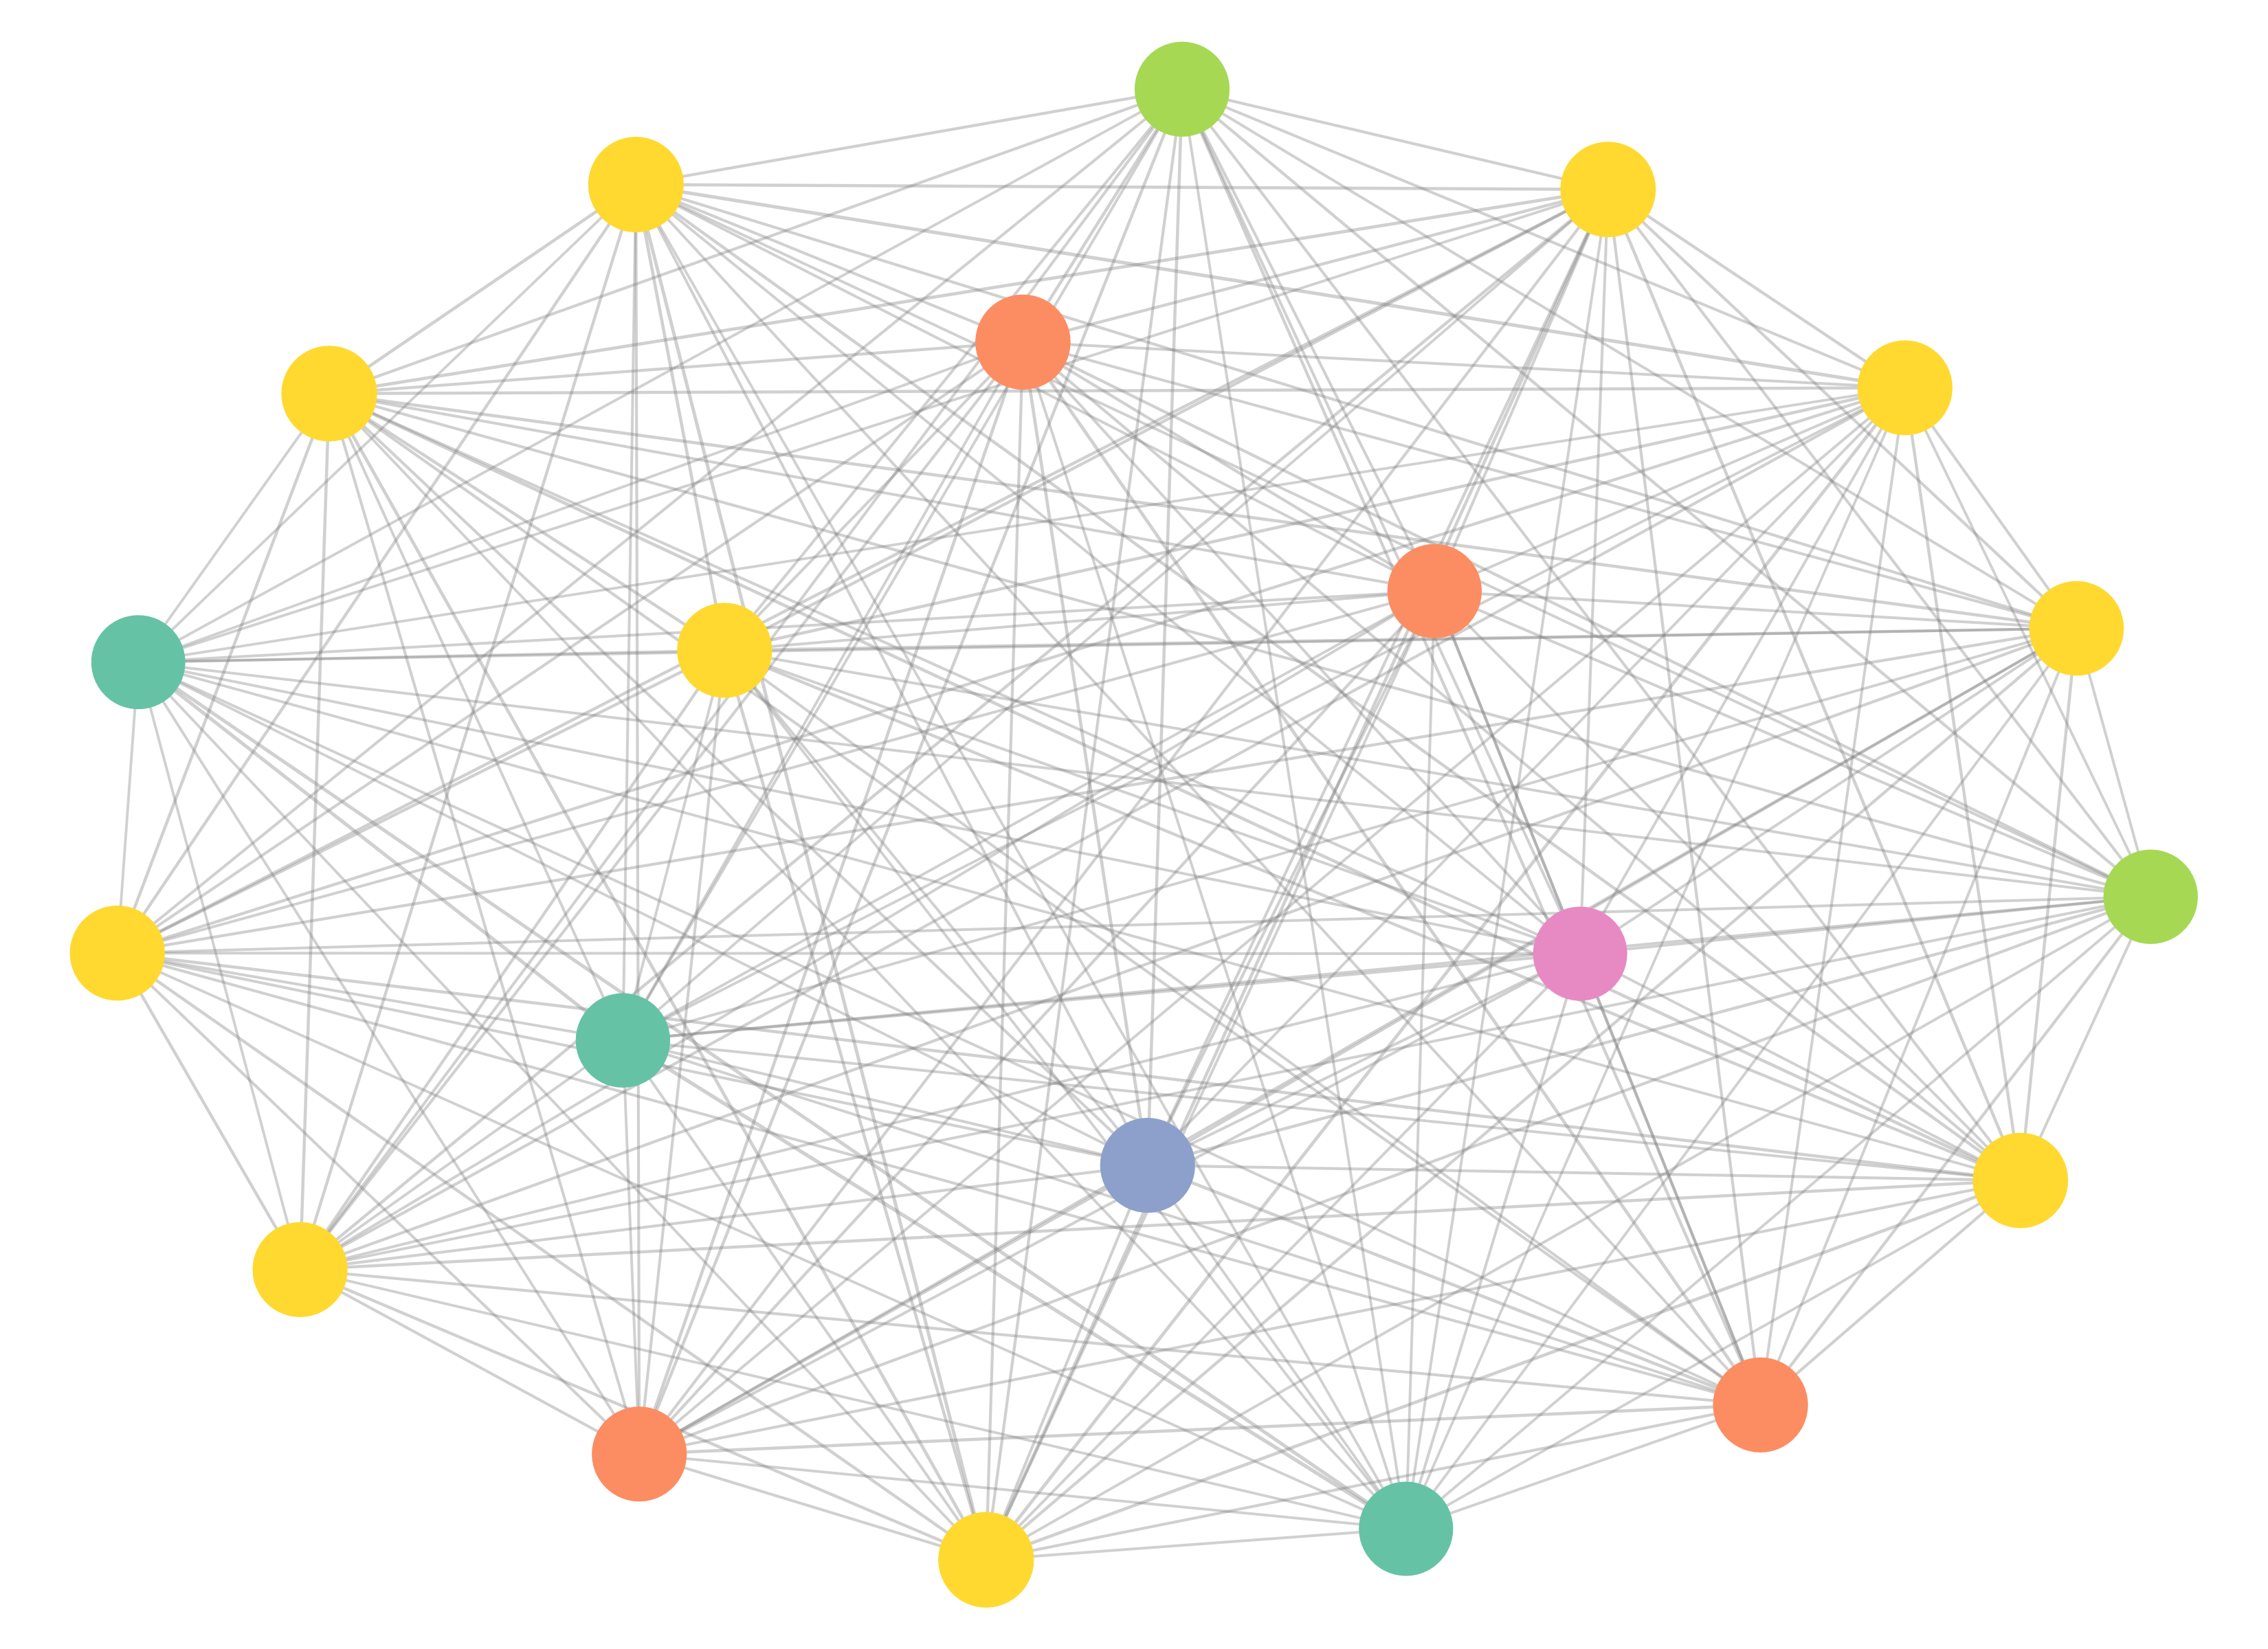
\includegraphics{plots/fig-rtn95.png}

}

}

\subcaption{\label{fig-rtn95}Extreme upper quantile (95th percentile)}
\end{minipage}%
\newline
\begin{minipage}[t]{\linewidth}

{\centering 

\raisebox{-\height}{

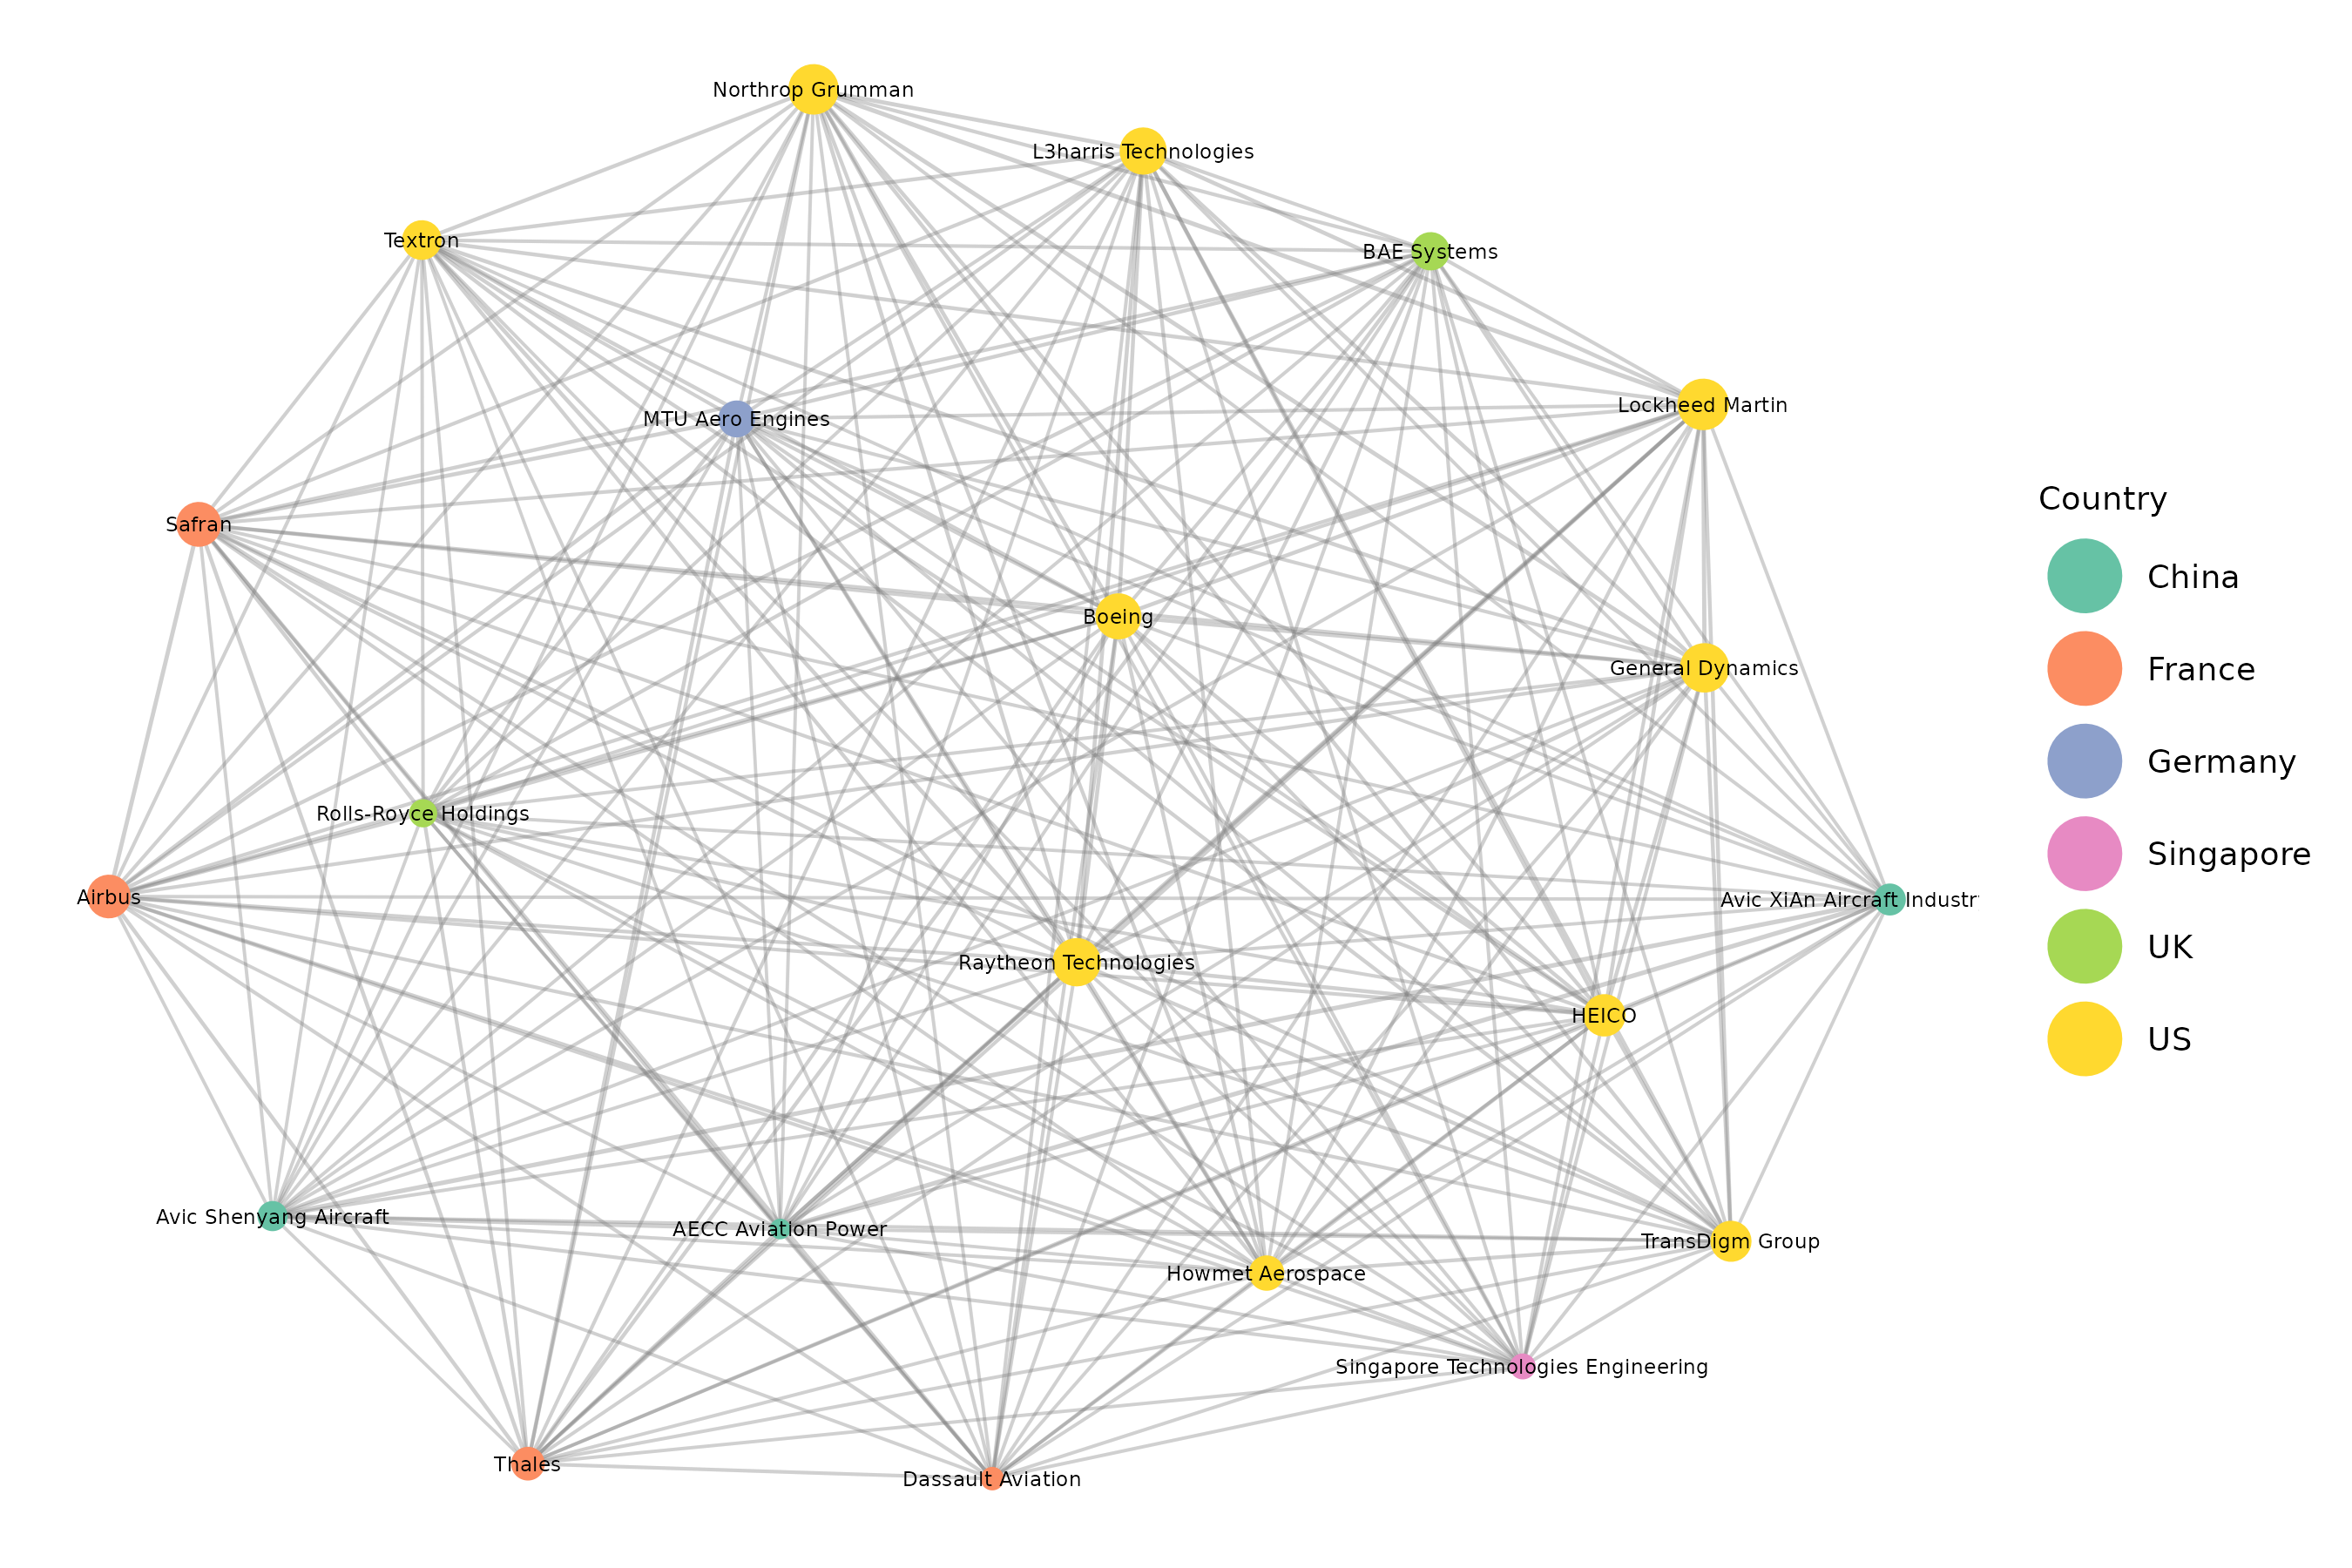
\includegraphics{plots/fig-rtn5.png}

}

}

\subcaption{\label{fig-rtn5}Extreme lower quantile (5th percentile)}
\end{minipage}%

\caption{\label{fig-rtn}Network topology of return spillover at various
quantiles}

\end{figure}

\hypertarget{volatility-spillovers}{%
\subsubsection{Volatility spillovers}\label{volatility-spillovers}}

Moving to the network of volatility spillovers, Figure~\ref{fig-vol}
exhibits a similar pattern to those for the return spillovers. Weak
bilateral spillovers characterise the extreme upper quantile, and the
strongest pairwise spillovers occur at the median quantile. Again, we
observe the most robust volatility linkages between Chinese companies,
followed by volatility linkages between US companies. Strong volatility
linkages between Chinese companies are also apparent at the extreme
lower quantile. Huang et al.~(2021) constructed a tail risk spillover
network for China's industry sectors. They showed that the national
defence sector is defined as a `downstream' sector due to its position
in the industrial chain. It is found that it has relatively high
volatility compared to other leading industries. Bu et al.~(2019)
analysed movement in the Chinese stock market using a causal network
method, finding that investors are concerned with risk and return in
normal periods but are only concerned about risk in crisis periods.
Furthermore, we observe similar differences between low and high
volatility market conditions in terms of the aggregate spillover effect
sizes and distributional differences.

\begin{figure}[H]

\begin{minipage}[t]{0.50\linewidth}

{\centering 

\raisebox{-\height}{

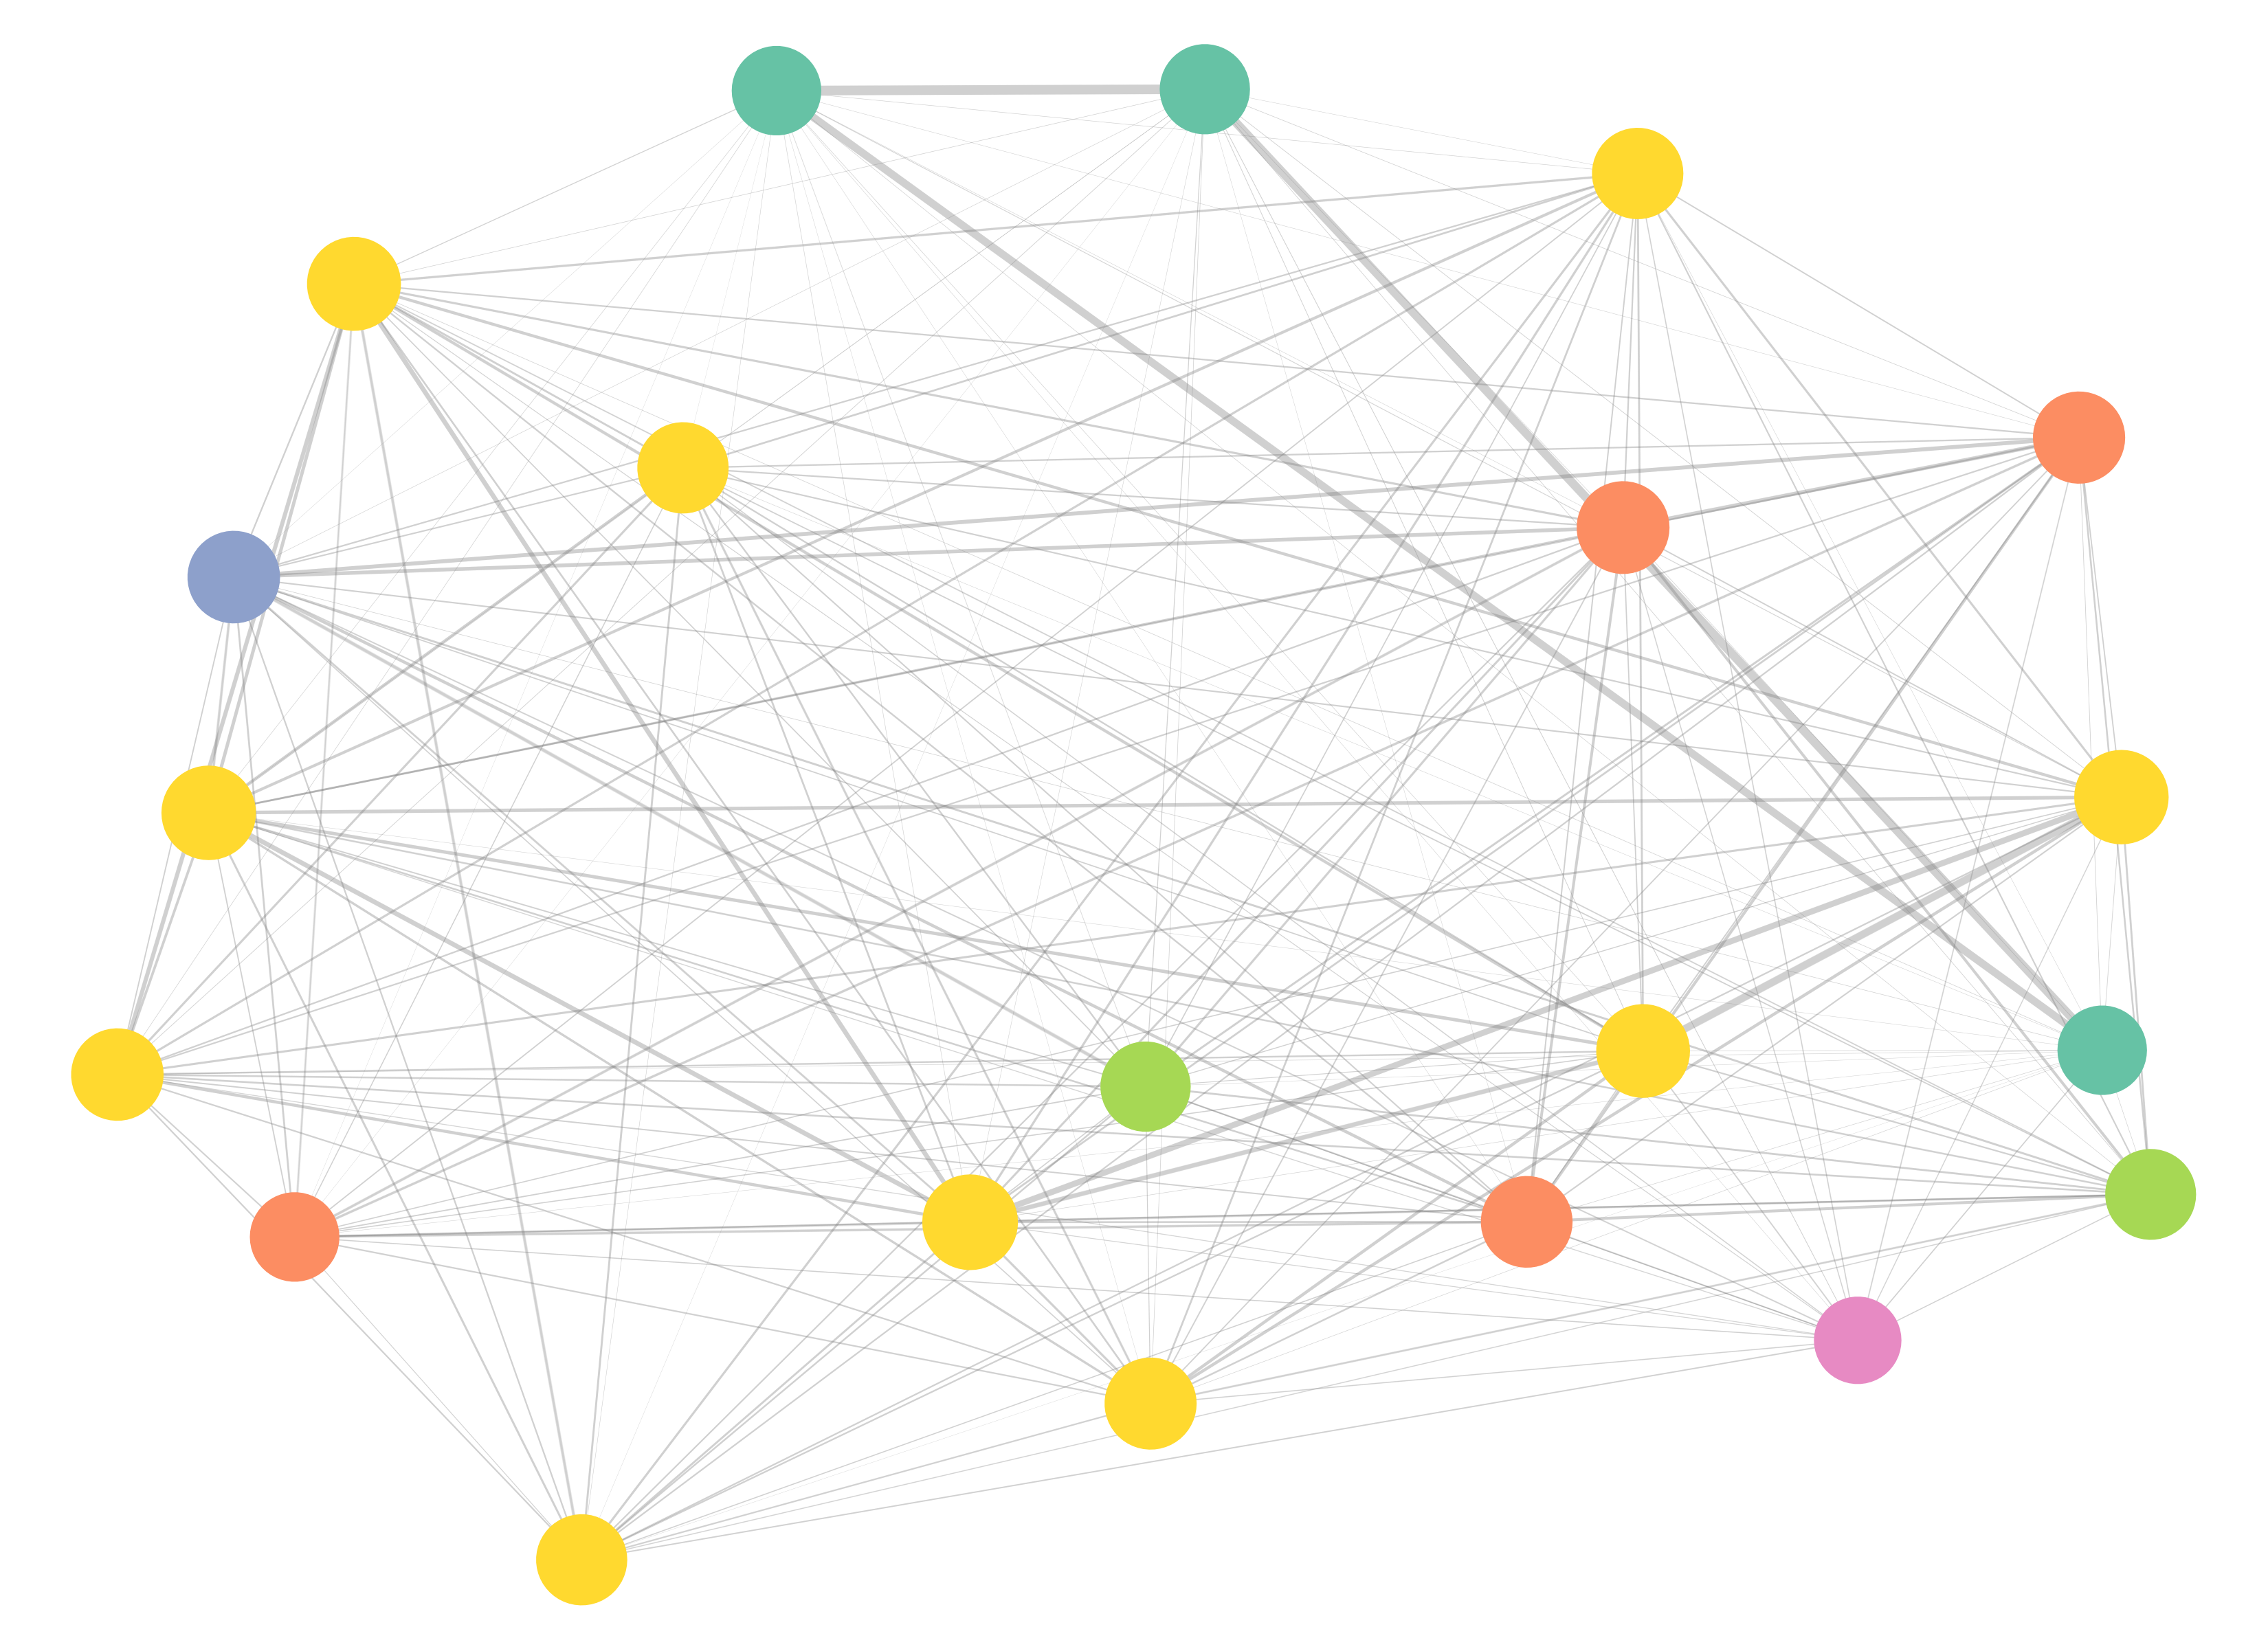
\includegraphics{plots/fig-vol50.png}

}

}

\subcaption{\label{fig-vol50}Middle quantile (50\textsuperscript{th}
Percentile)}
\end{minipage}%
%
\begin{minipage}[t]{0.50\linewidth}

{\centering 

\raisebox{-\height}{

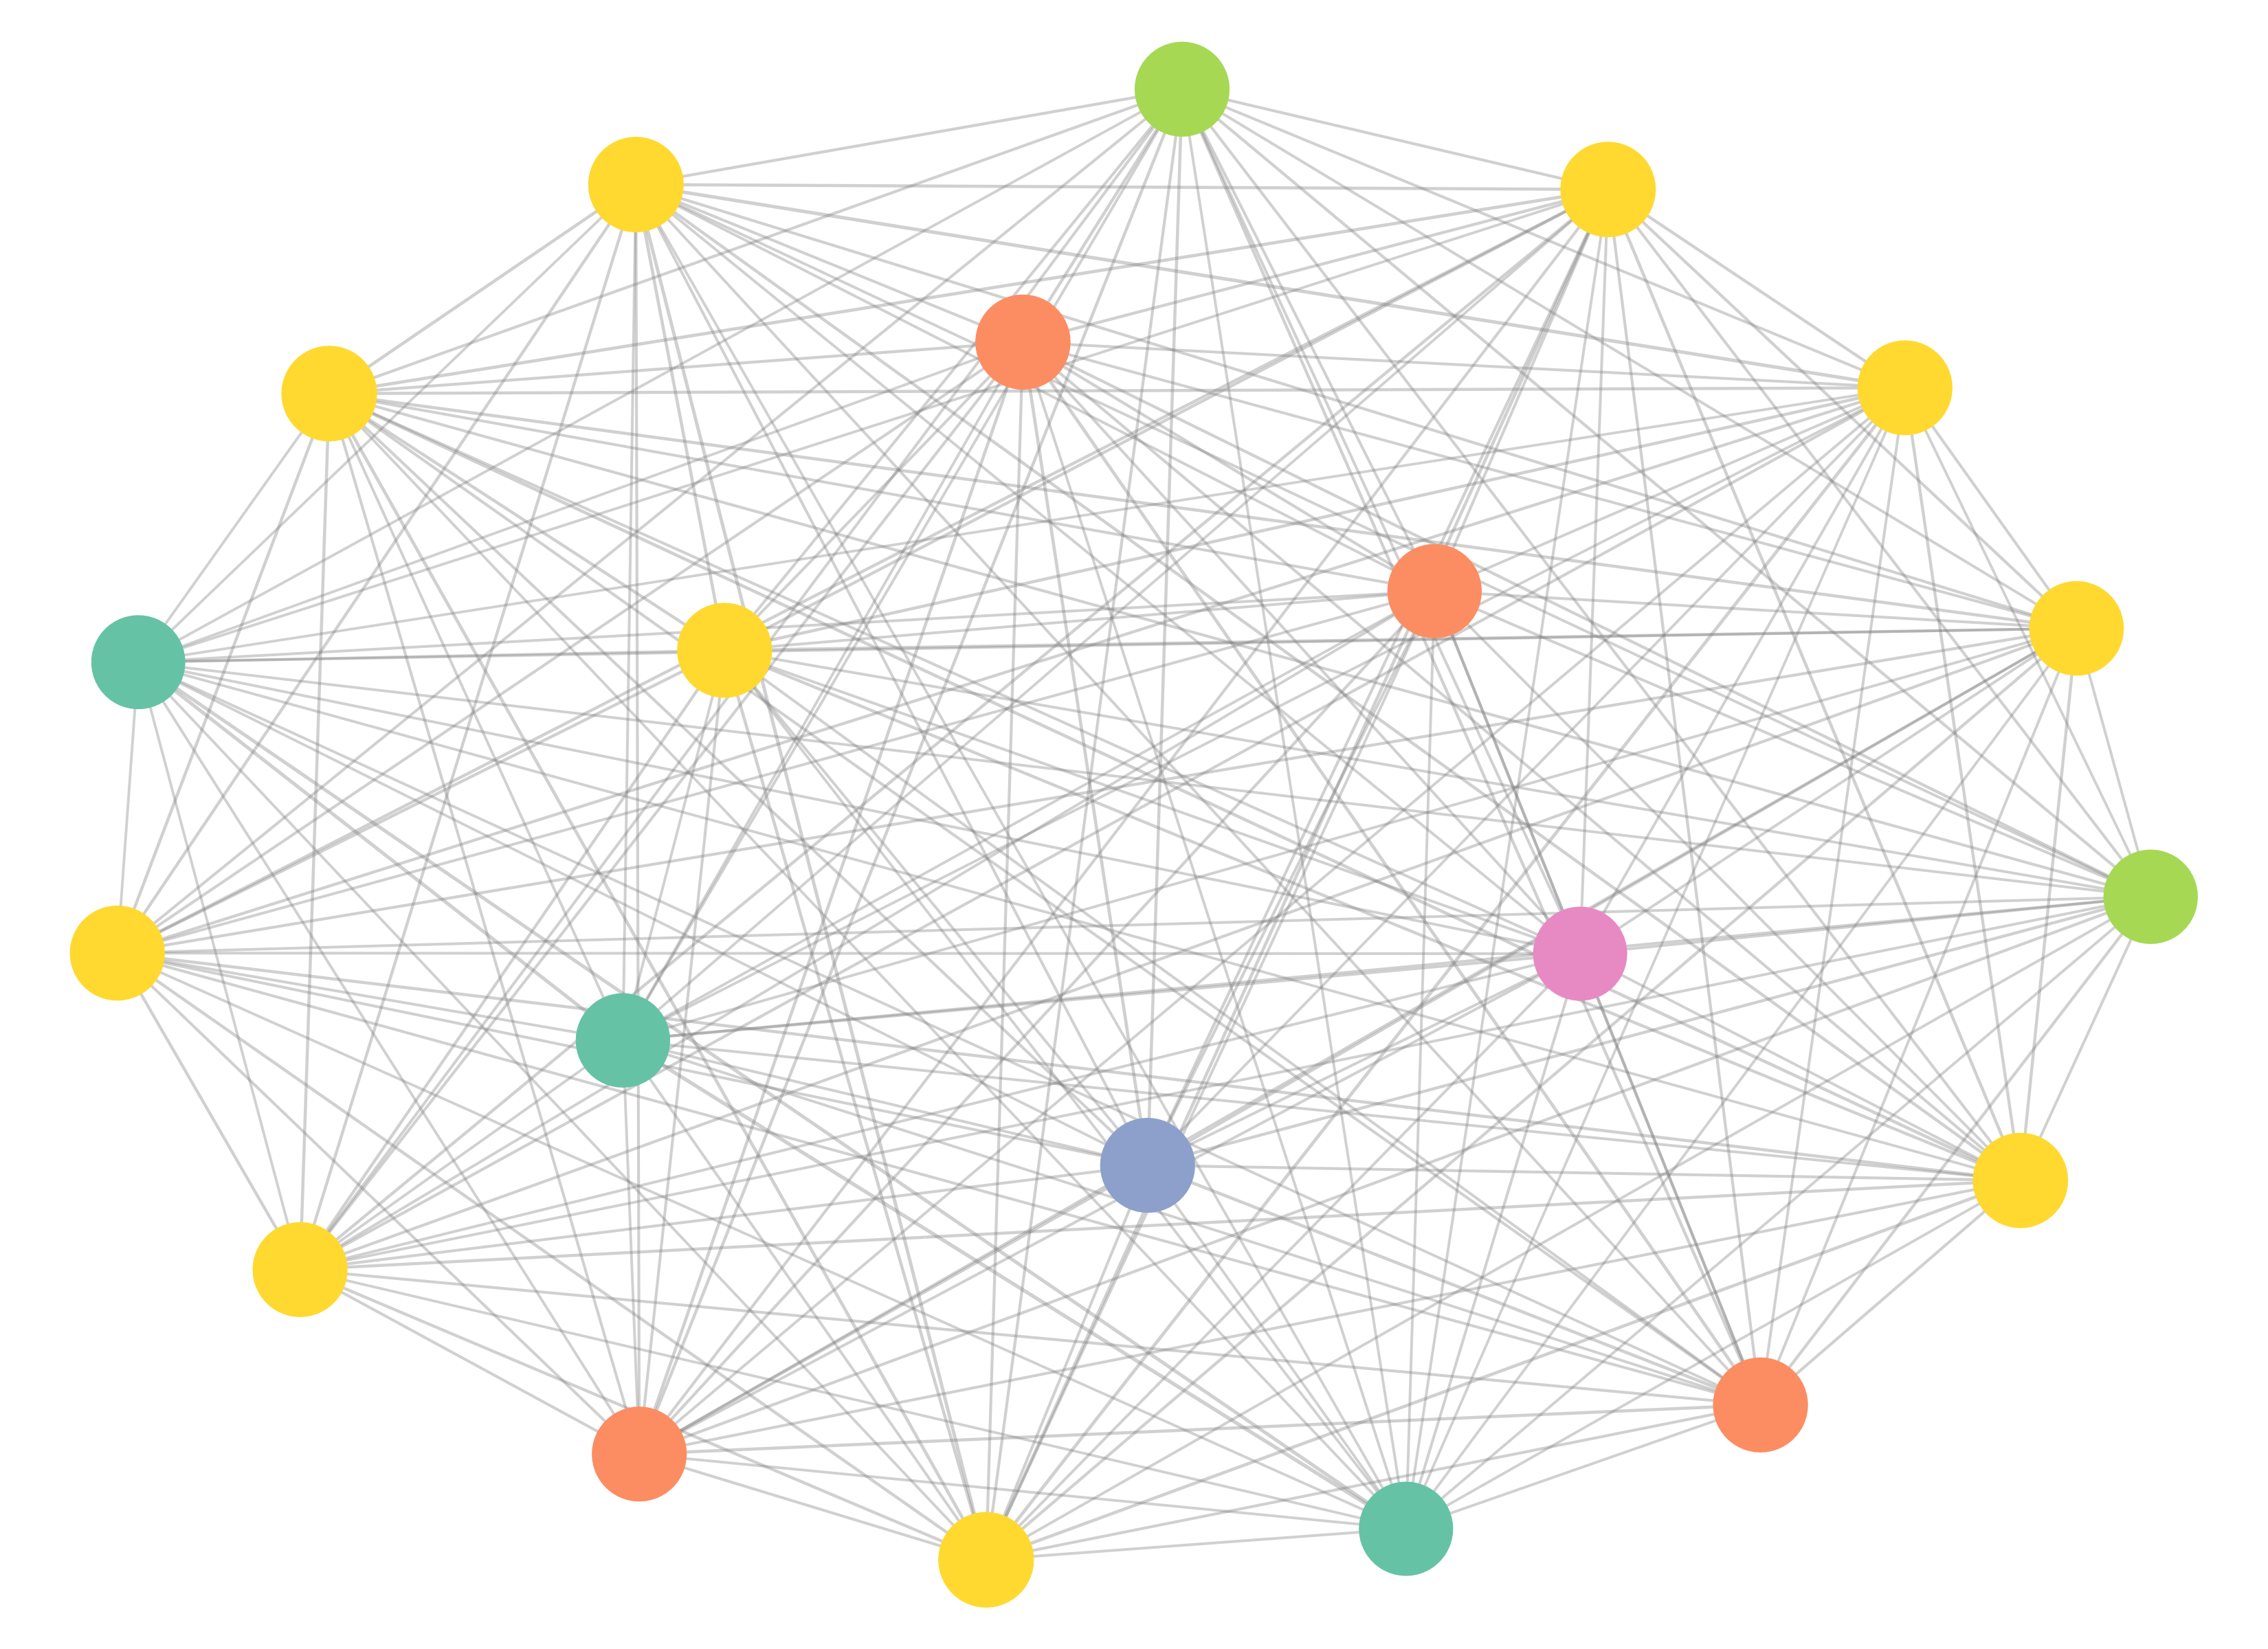
\includegraphics{plots/fig-rtn95.png}

}

}

\subcaption{\label{fig-vol95}Extreme upper quantile
(95\textsuperscript{th} percentile)}
\end{minipage}%
\newline
\begin{minipage}[t]{\linewidth}

{\centering 

\raisebox{-\height}{

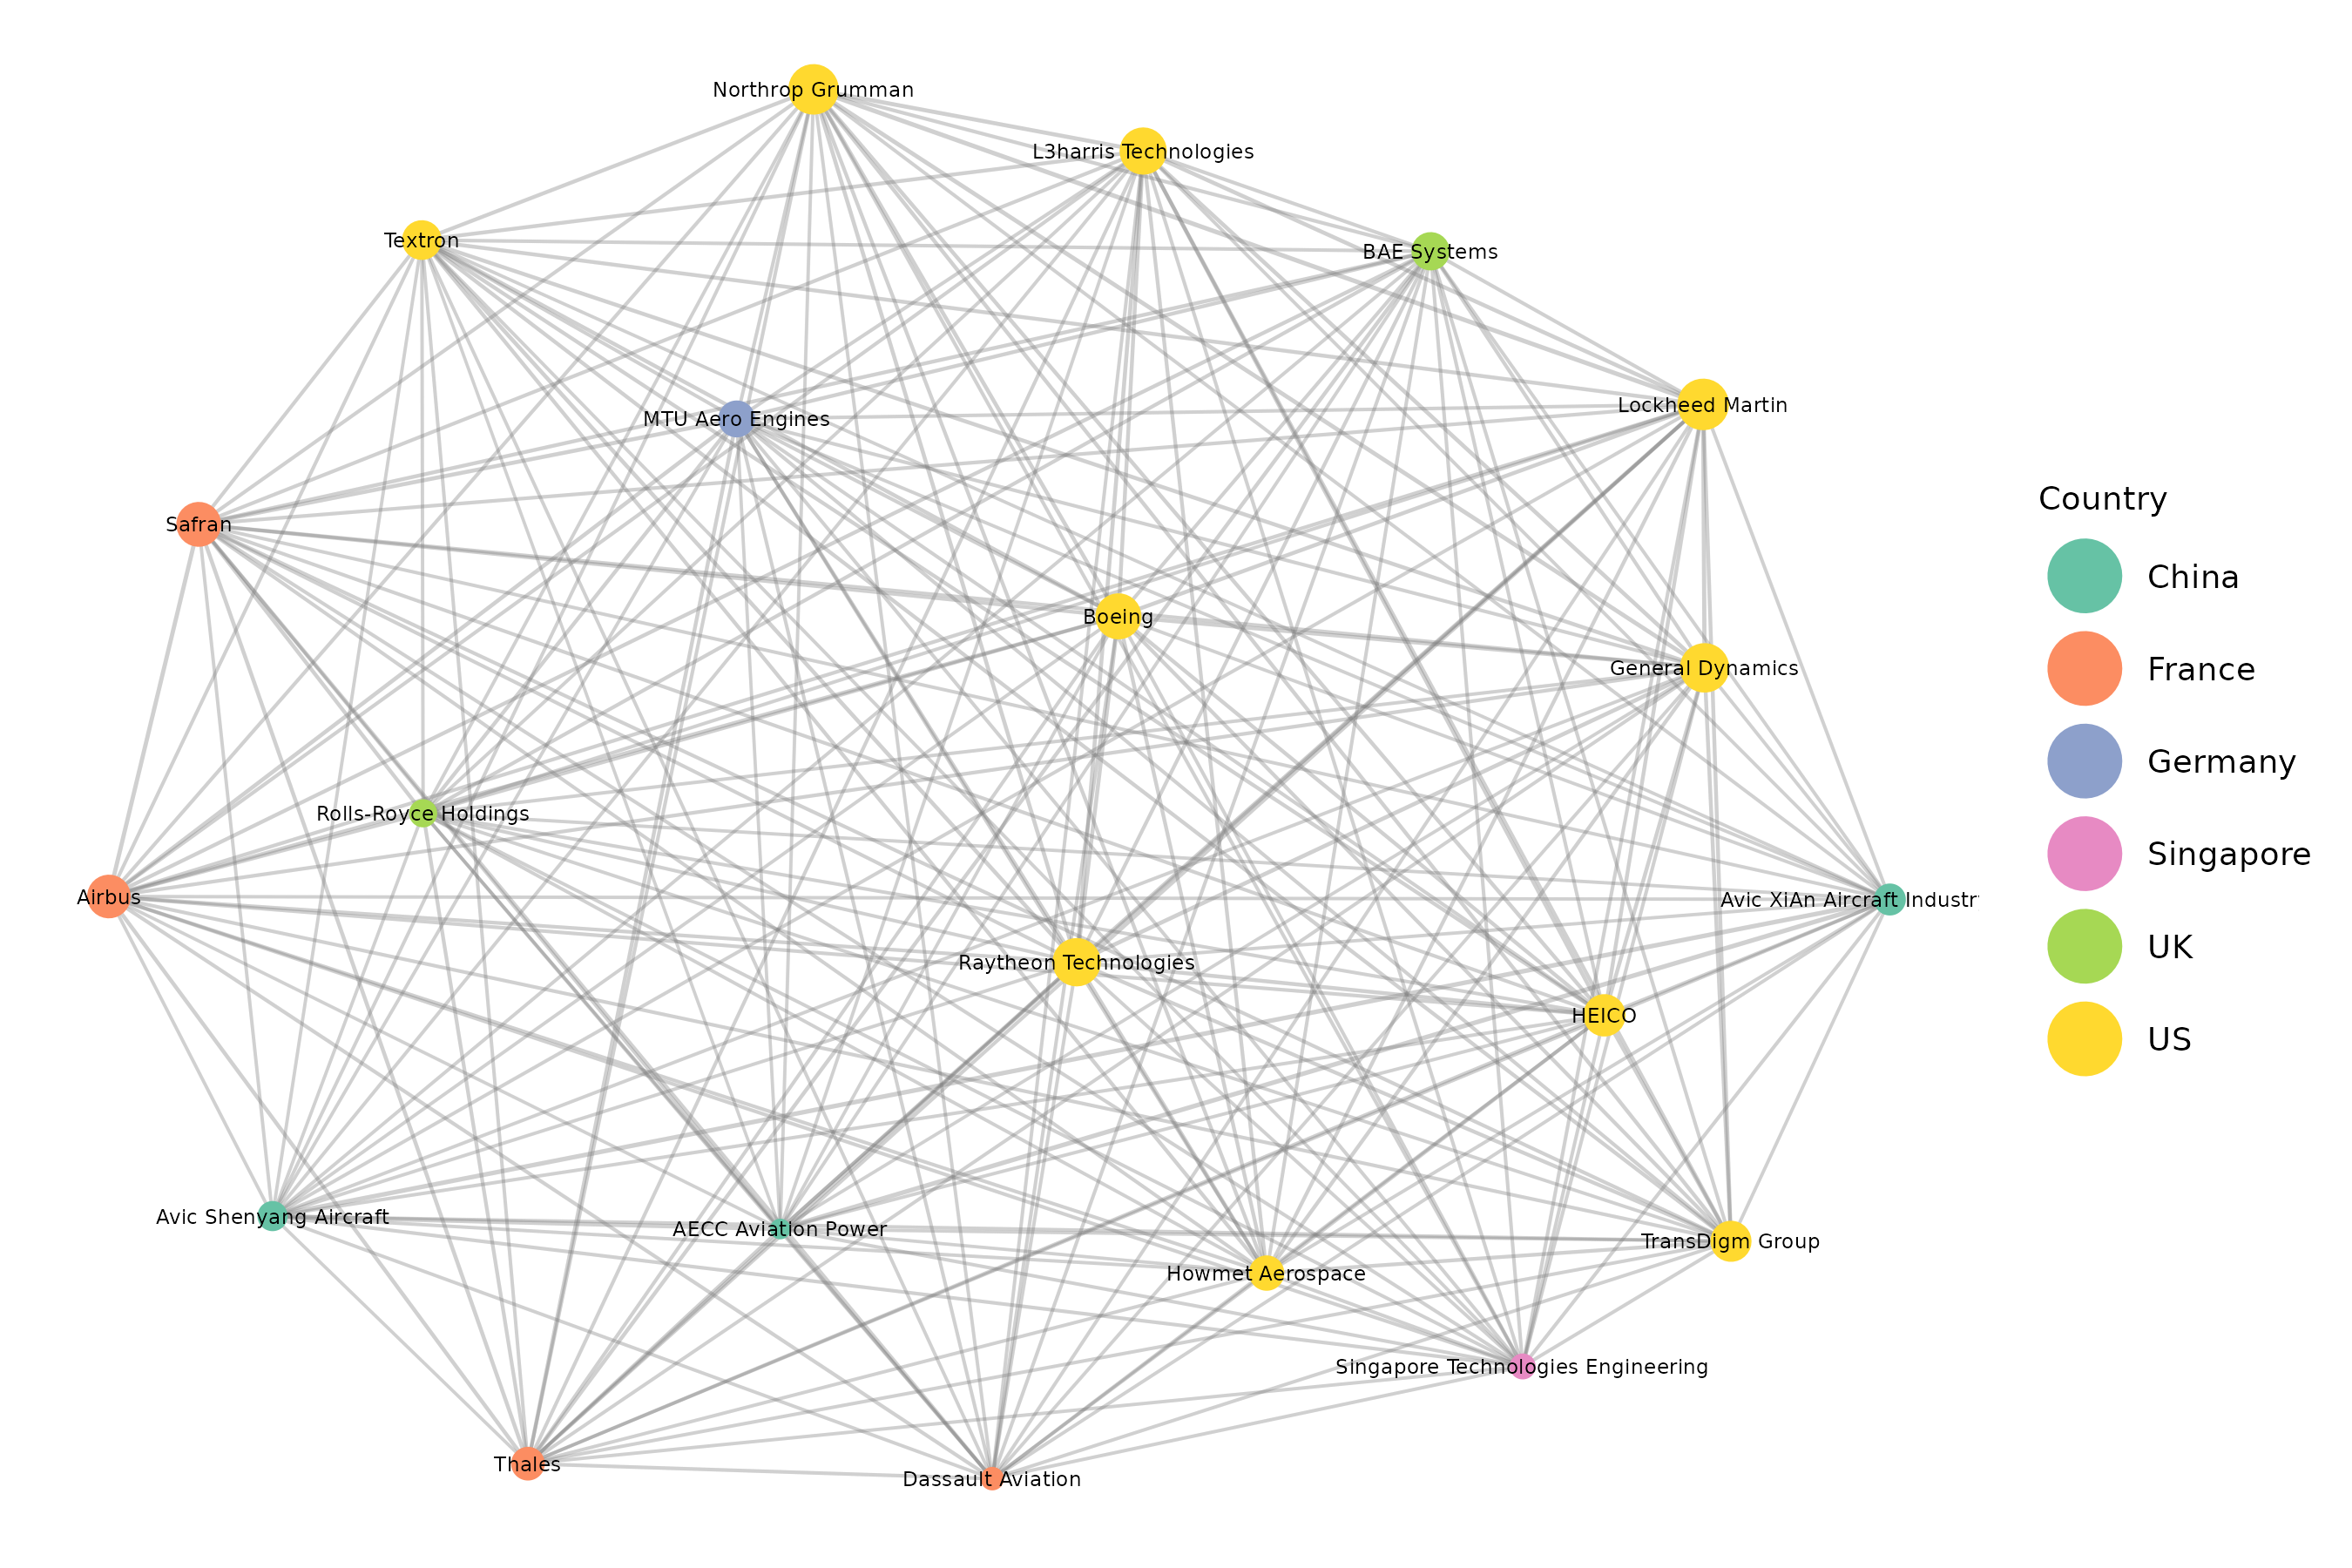
\includegraphics{plots/fig-rtn5.png}

}

}

\subcaption{\label{fig-vol5}Extreme lower quantile
(5\textsuperscript{th} percentile)}
\end{minipage}%

\caption{\label{fig-vol}Network topology of volatility spillover at
various quantiles}

\end{figure}

\hypertarget{time-varying-spillover-results}{%
\subsection{Time varying spillover
results}\label{time-varying-spillover-results}}

So far, we have analysed measures of connectedness for the entire sample
using the network topology visualisation. However, it is essential to
illustrate meaningful time variation in the returns and volatility
spillover effects of A\&D stocks under various market conditions.
Furthermore, bilateral spillover of idiosyncratic risk seems stronger
for both returns and volatility series, which reflect the
interconnectedness across A\&D stocks. However, it is important to note
that restricting the network analysis to the middle of the distribution
will not capture the full extent of dependence when large negative
return and large positive return shocks occur (i.e.under extreme market
conditions and events) as well as very low and very high volatility
shocks manifest. Therefore, in this section, we conduct a rolling
analysis with a quantile VAR to capture the time variability in the
return and volatility spillovers in normal times (i.e.at the median of
the conditional distribution) and abnormal market conditions (i.e.~atthe
upper and lower tails of the conditional distribution). We use a fixed
window length of 200\footnote{Existing studies in the Deibold-Yilmaz
  network literature use windows ranging from 100-250 days. Sensitivity
  analysis has been done and available upon request.} days and a 10-step
forecast horizon. This will provide a comprehensive analysis of
connectedness at the center and in the left and right tail dependence.
This is conducted for both returns and volatility.

\hypertarget{total-system-connectivity}{%
\subsubsection{Total system
connectivity}\label{total-system-connectivity}}

\begin{figure}[H]

{\centering 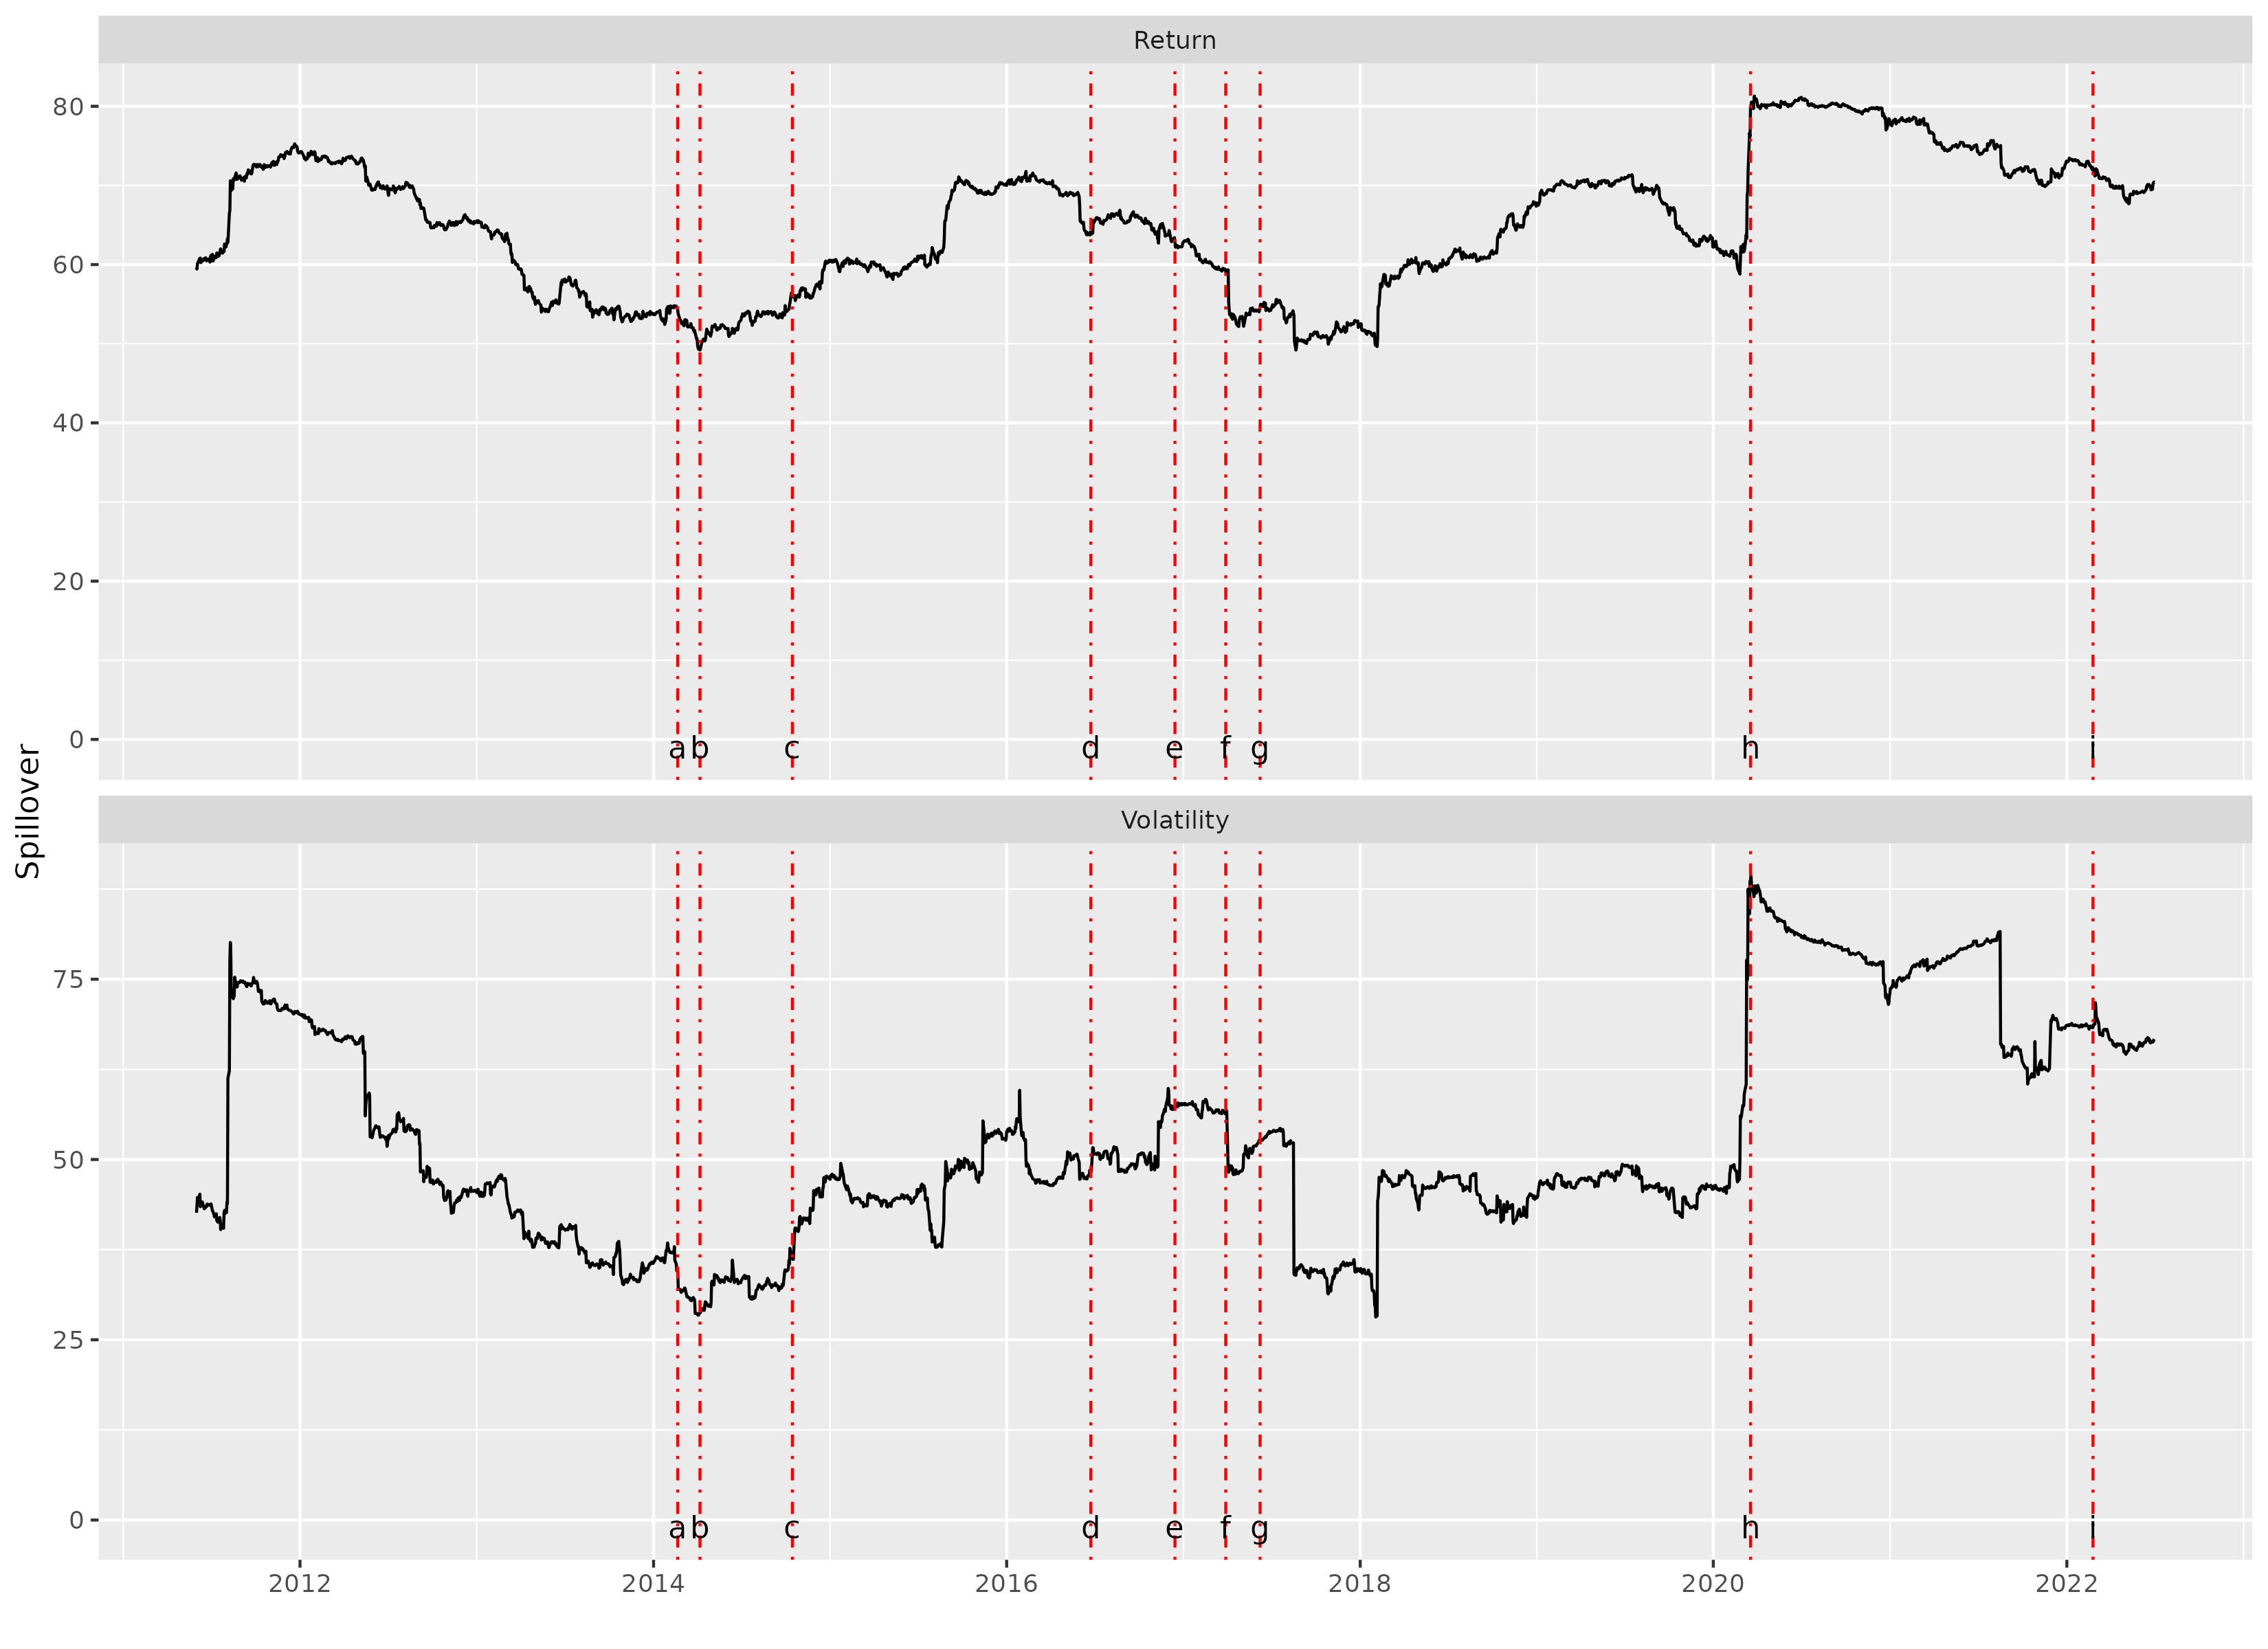
\includegraphics{plots/fig-TCI50.png}

}

\caption{\label{fig-TCI50}Total system connectedness at the conditional
Median (50\textsuperscript{th} Percentile)}

\end{figure}

\begin{figure}[H]

{\centering 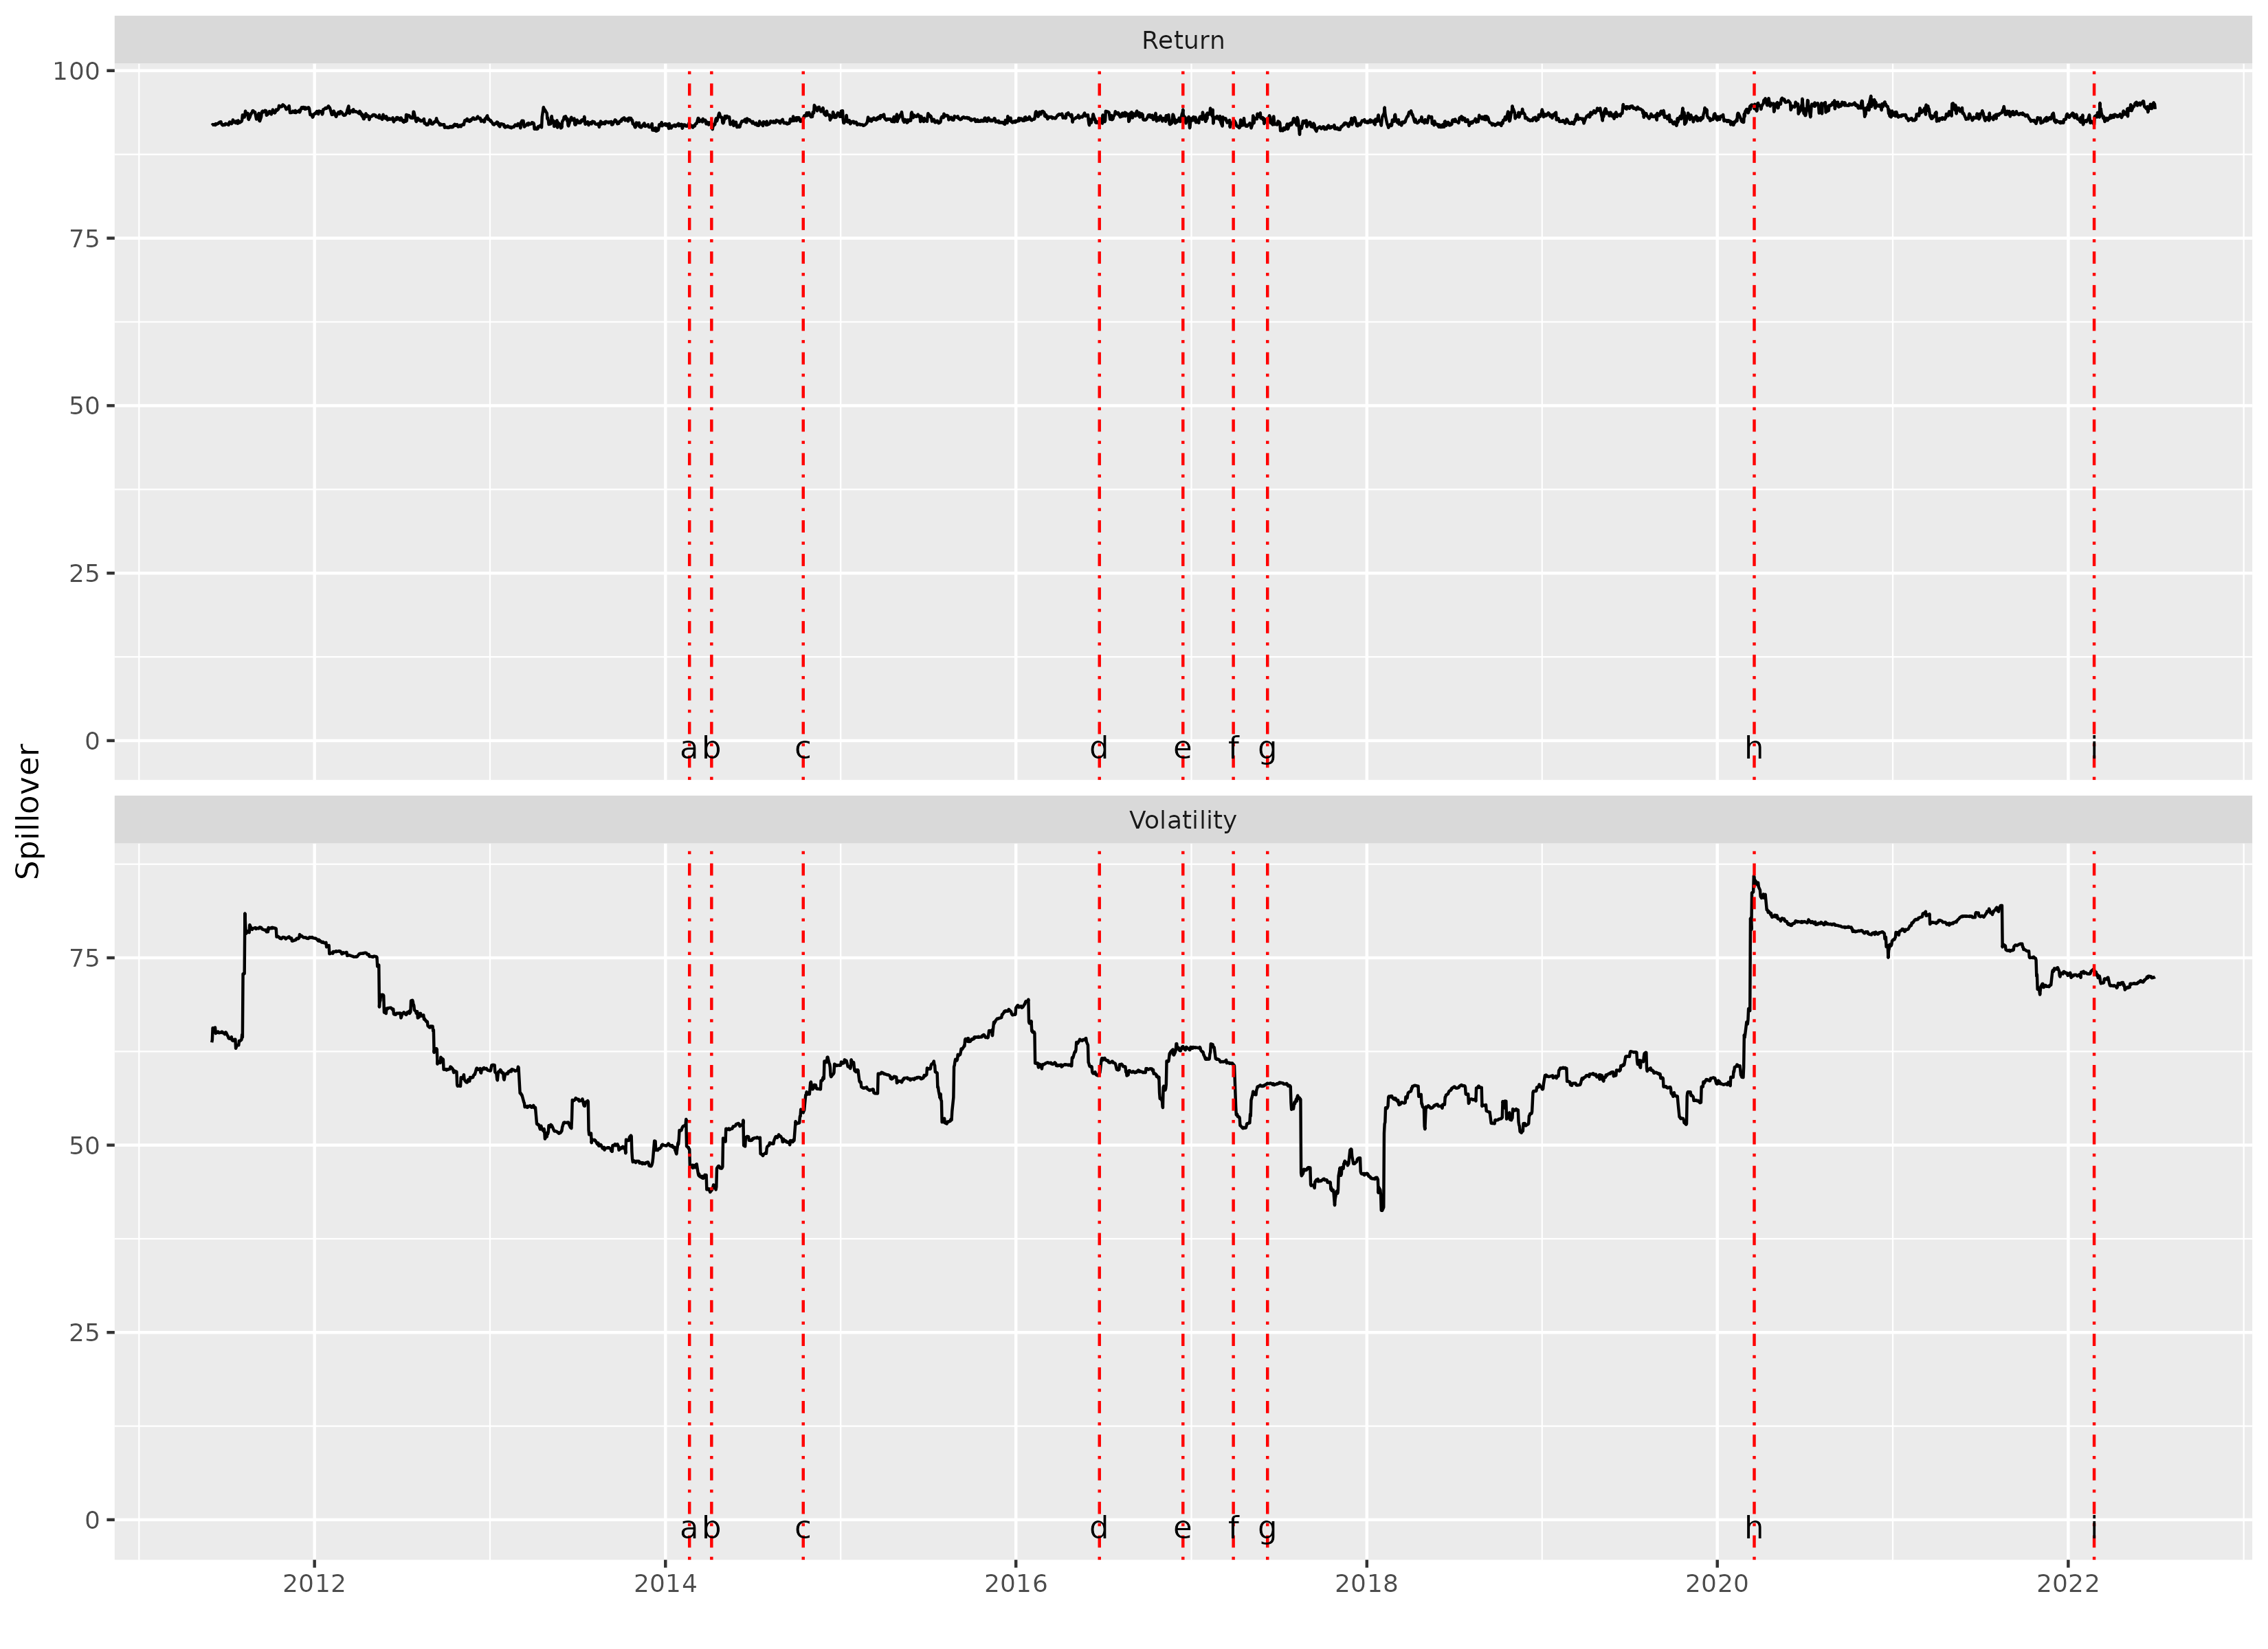
\includegraphics{plots/fig-TCI5.png}

}

\caption{\label{fig-TCI5}Total system connectedness at the
5\textsuperscript{th} percentile}

\end{figure}

\begin{figure}[H]

{\centering 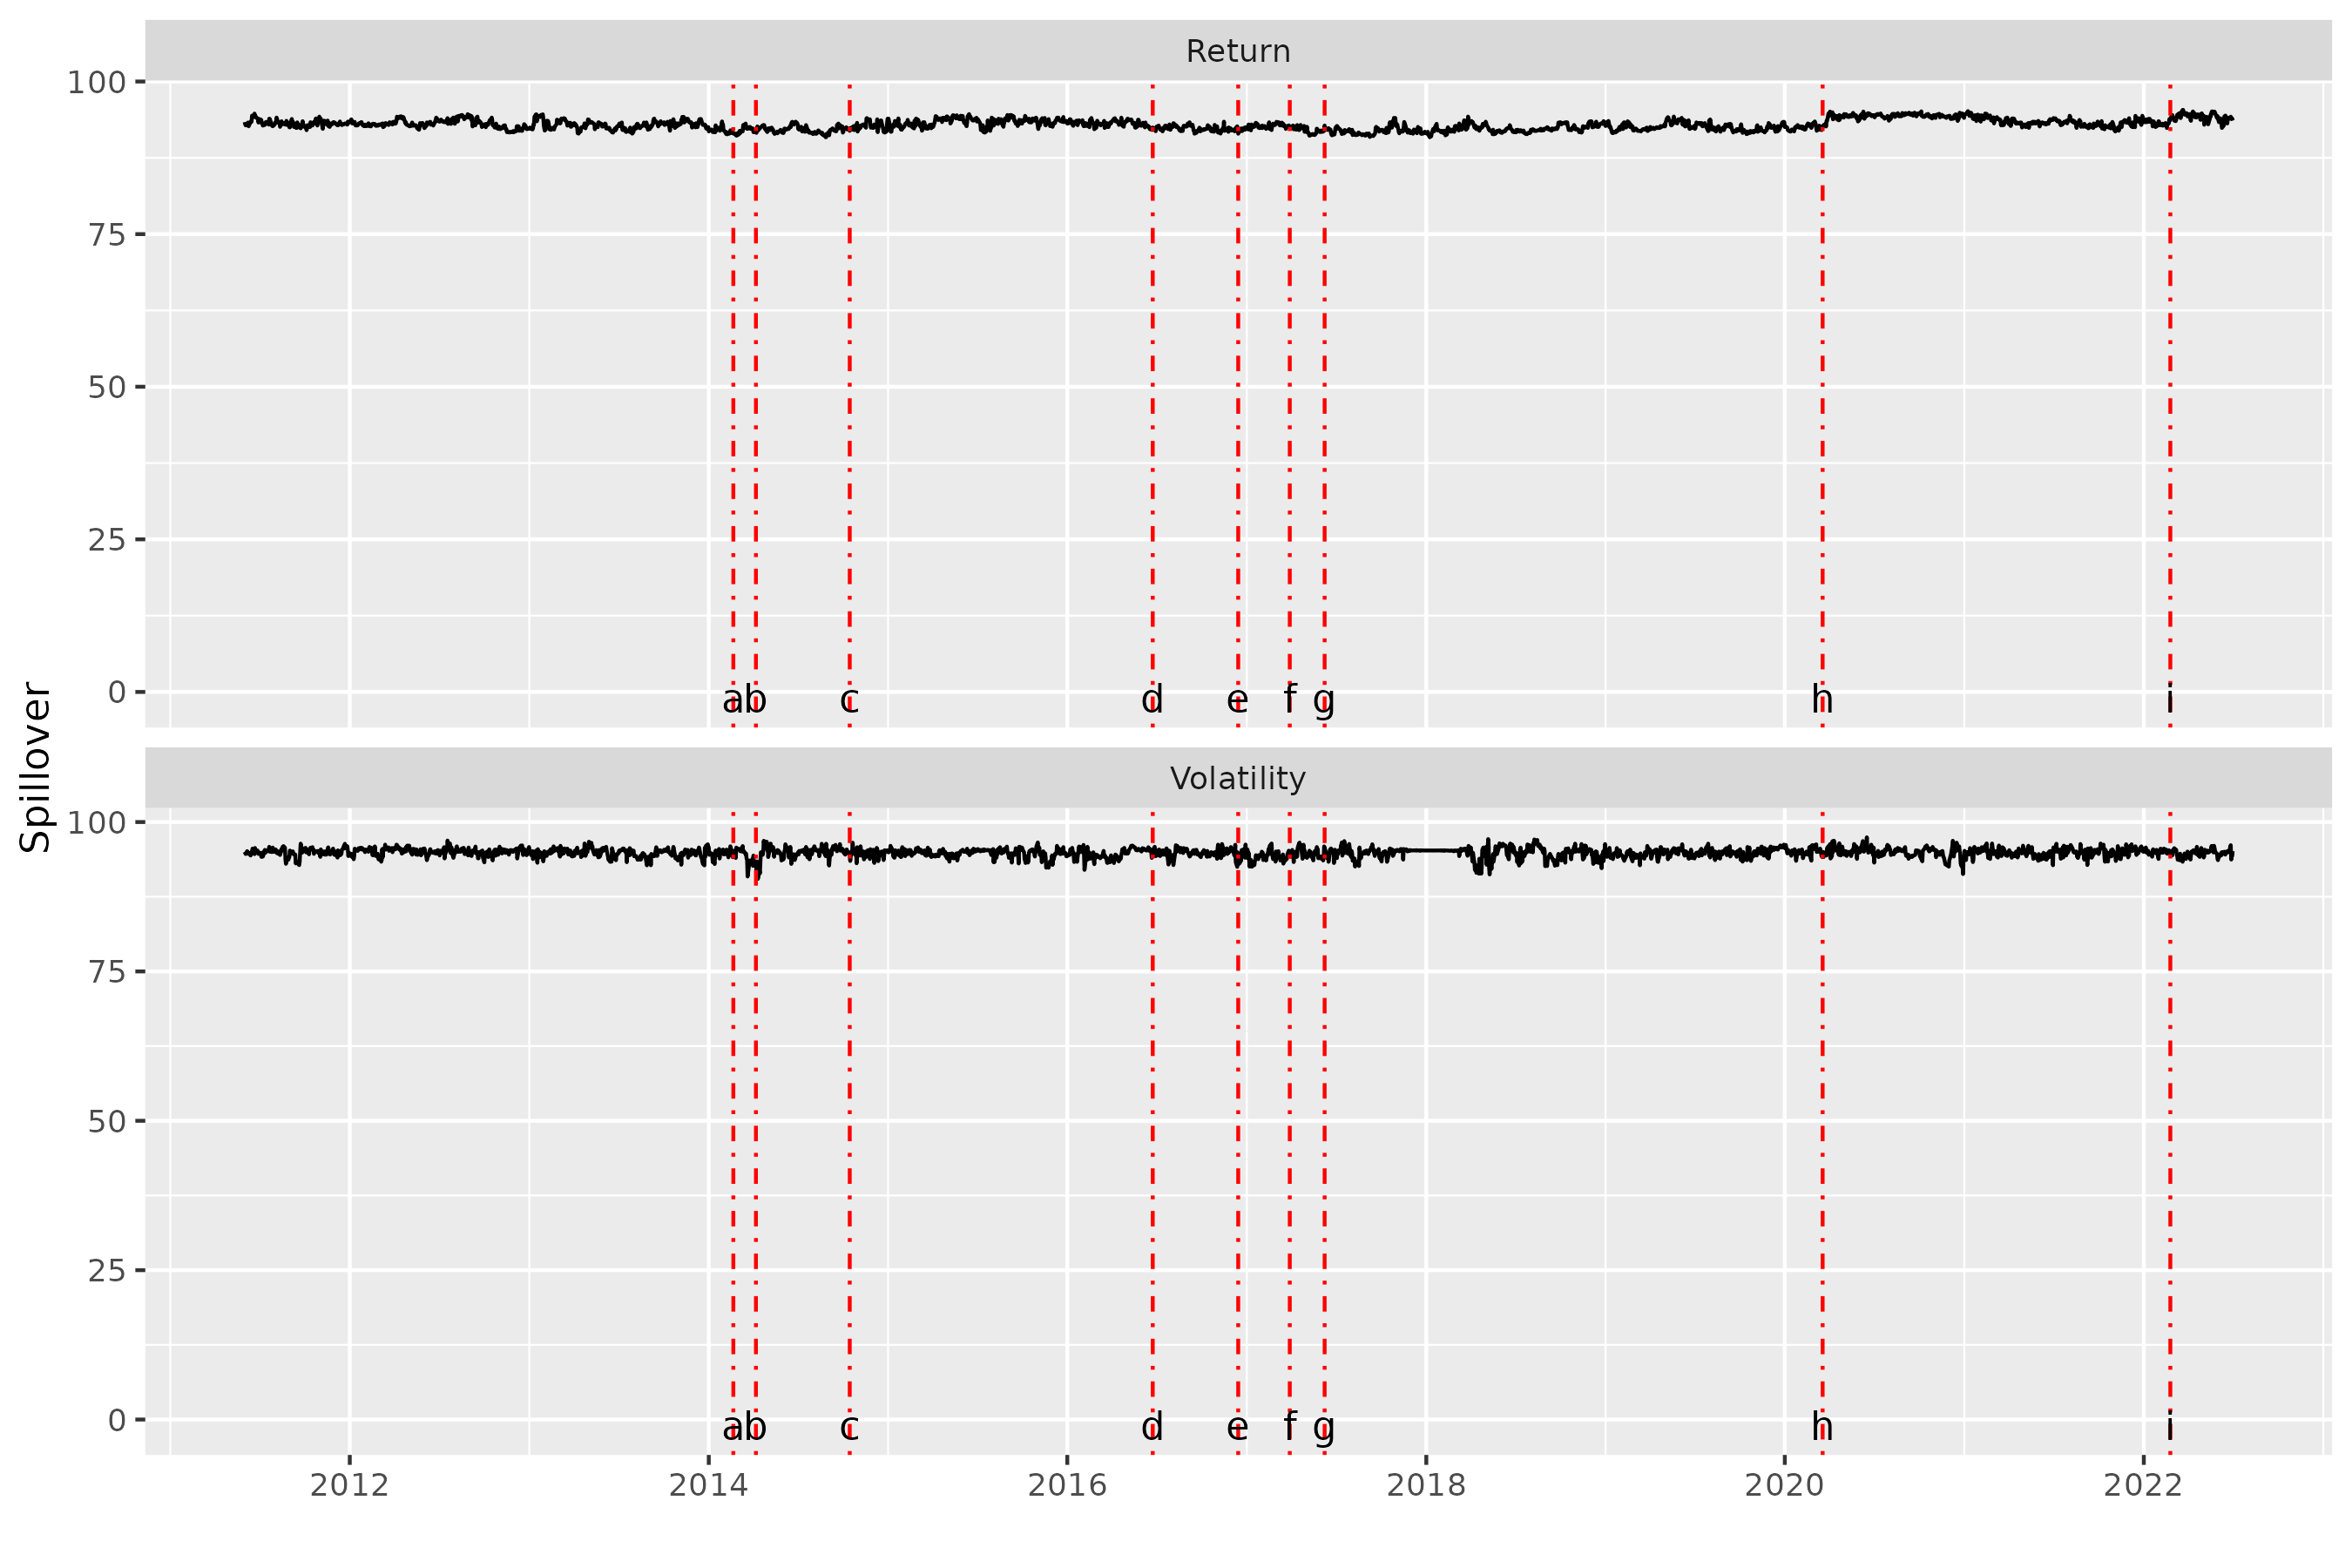
\includegraphics{plots/fig-TCI95.png}

}

\caption{\label{fig-TCI95}Total system connectedness at the
95\textsuperscript{th} percentile}

\end{figure}

\begin{figure}[H]

{\centering 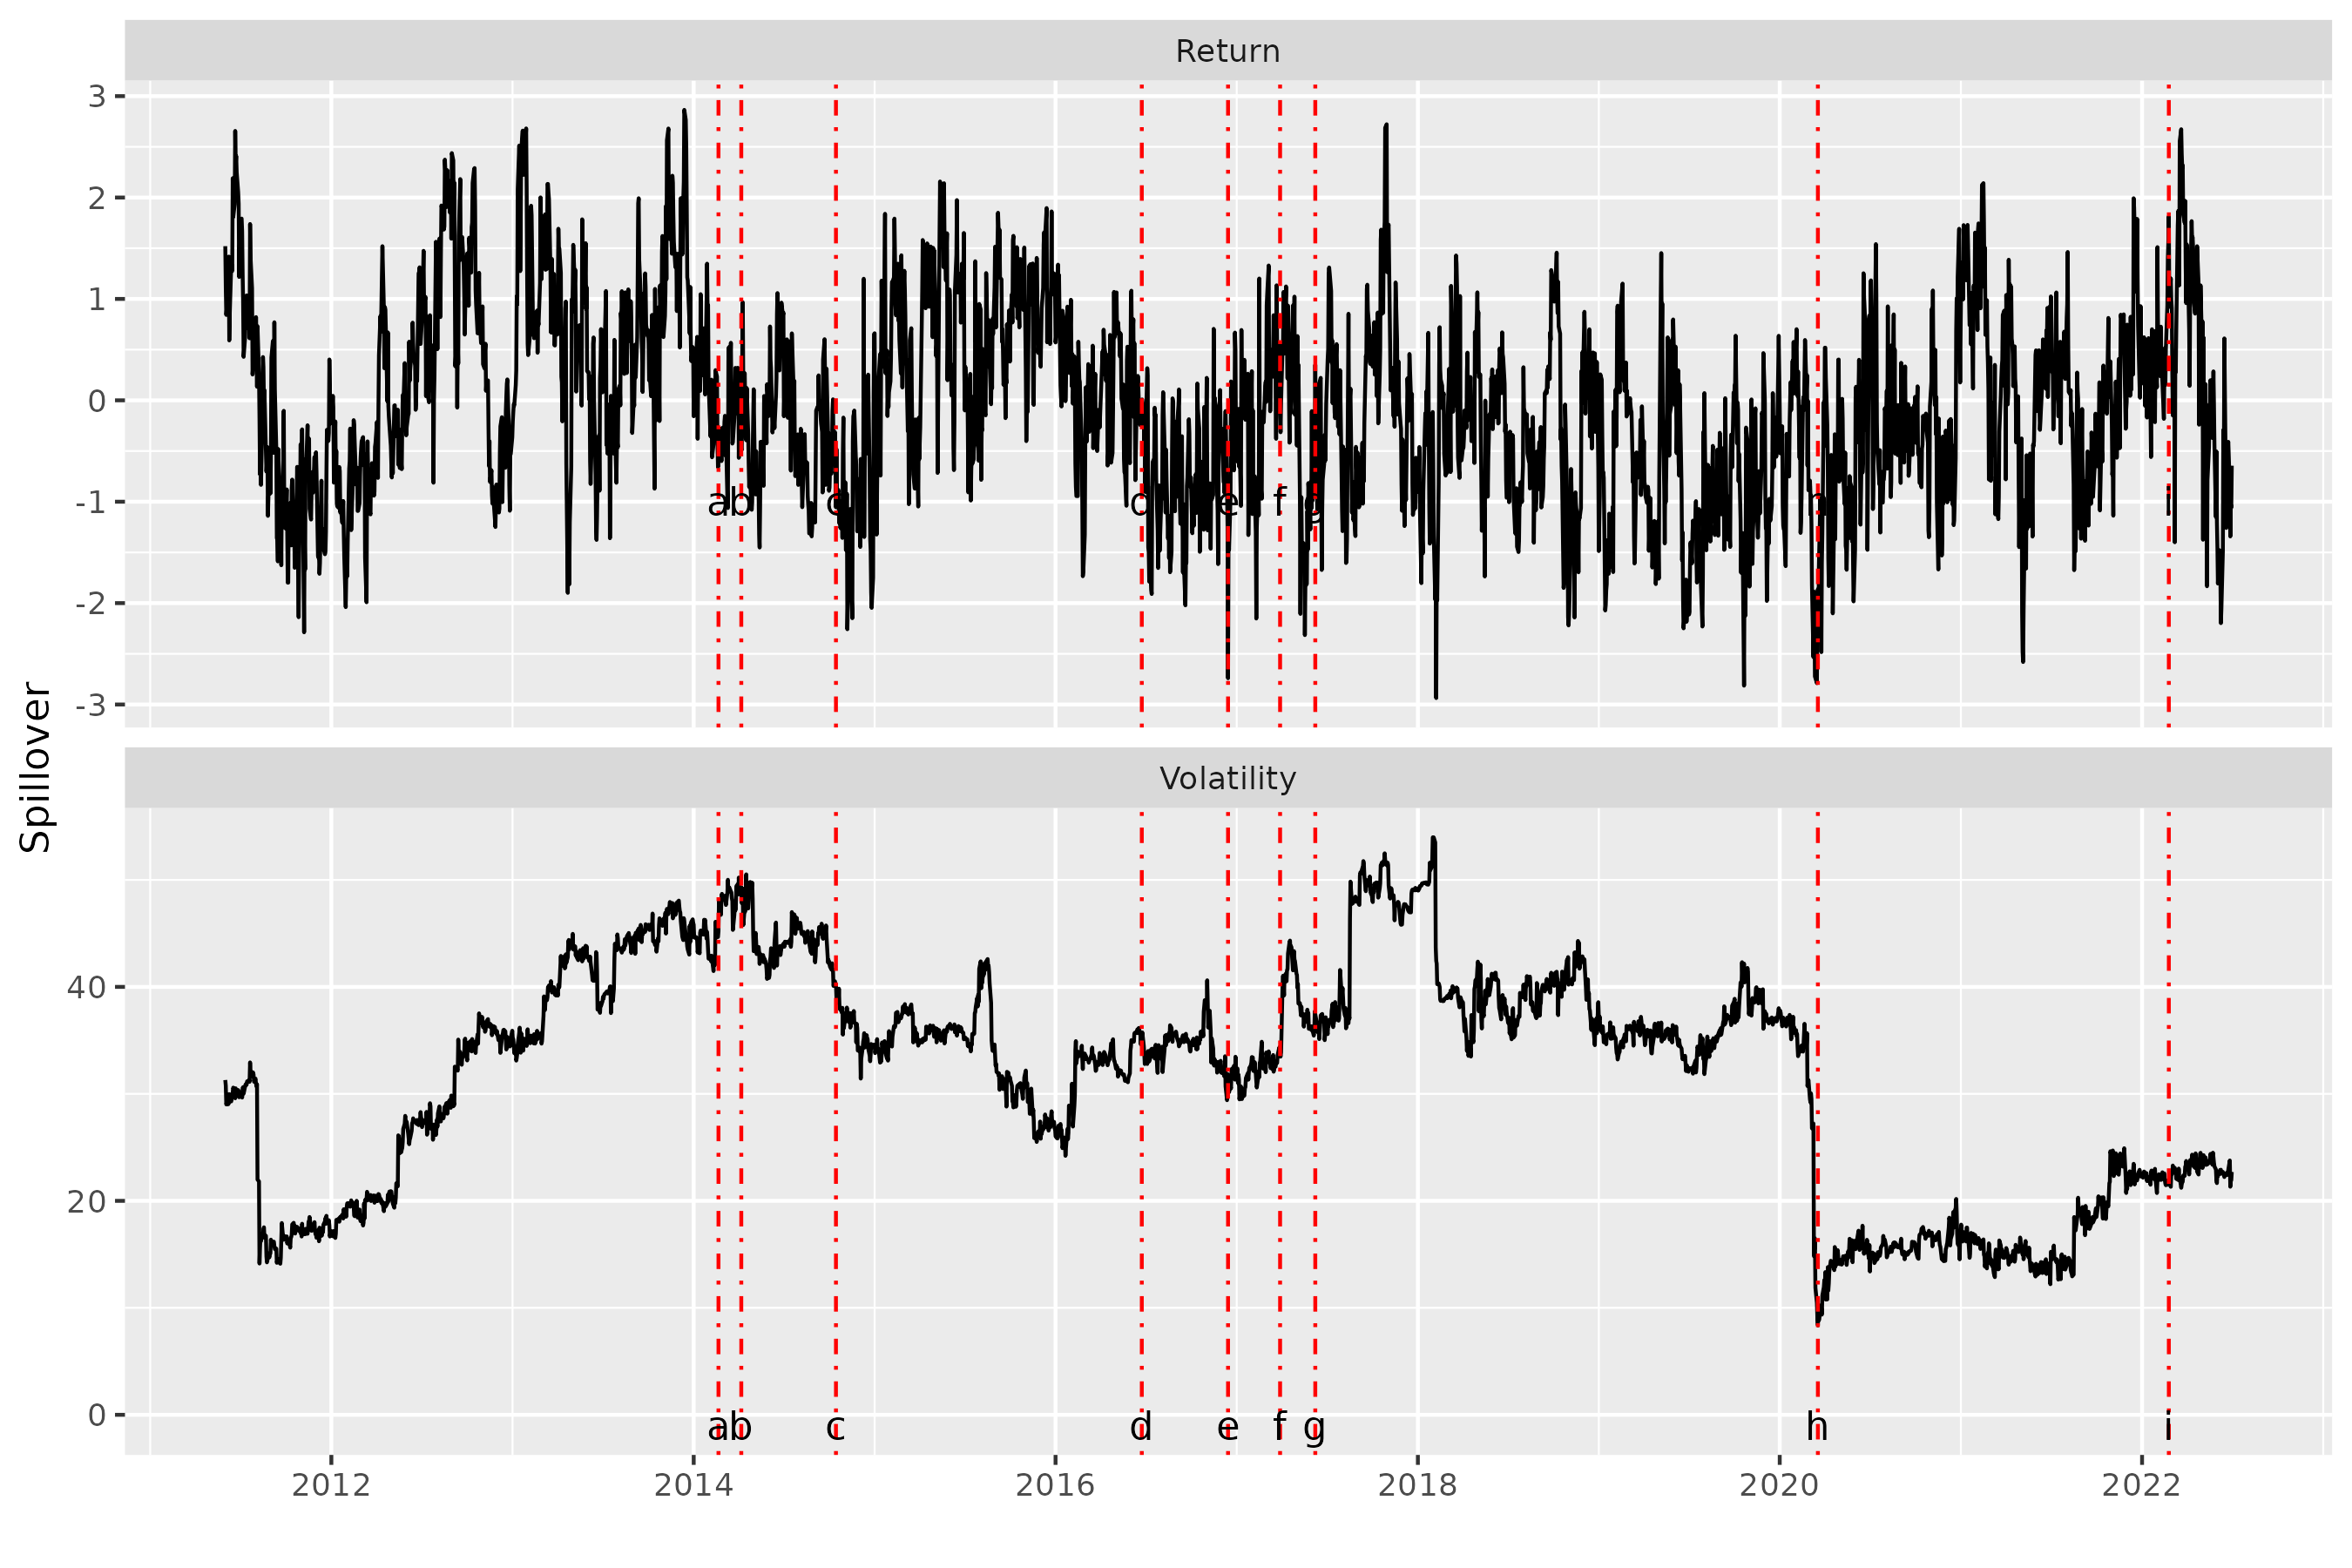
\includegraphics{plots/fig-TCIrtd.png}

}

\caption{\label{fig-TCIrtd}Relative tail dependence (RTD), the
difference between 95\textsuperscript{th} minus 5\textsuperscript{th}
percentile}

\end{figure}

Figure~\ref{fig-TCI50}, Figure~\ref{fig-TCI5}, Figure~\ref{fig-TCI95},
compare the total connectedness of returns and volatility at various
quantiles. Vertical red dashed lines denote the dates of some important
events, which are described in Table~\ref{tbl-dates}.

\hypertarget{tbl-dates}{}
\begin{table}[H]
\caption{\label{tbl-dates}Important Dates }\tabularnewline

\centering
\begin{tabular}[t]{lll}
\toprule
label & date & description\\
\midrule
a & 2014-02-20 & Russia began annexation of Crimea\\
b & 2014-04-07 & Start of war in Donbas by pro-Russian activists\\
c & 2014-10-15 & October 2014 flash crash\\
d & 2016-06-23 & Brexit referendum\\
e & 2016-12-14 & Federal Reserve raises interest rates\\
\addlinespace
f & 2017-03-29 & the United Kingdom invokes article 50 of the Lisbon Treaty\\
g & 2017-06-08 & snap election held in the United Kingdom\\
h & 2020-03-18 & Dash for cash crisis in bond market peaks\\
i & 2022-02-24 & Russia initiated a special military operation in Donbas\\
\bottomrule
\end{tabular}
\end{table}

The TOTAL connectedness index at the conditional median (a measure of
the average connectedness) and extremes for returns and volatility
systems are presented in Figure~\ref{fig-TCI50}. In normal conditions
the connectedness in the returns system tends to be larger than that of
the volatility system of defense stocks. The connectedness reaches its
peak at point h (the `dash for cash' event) at the beginning of the
COVID-19 pandemic. Importantly, while the connectedness levels are
greater in the returns system the volatility system connectedness
exhibits higher sensitivity to shocks, with the largest regime shift at
point h.

Figure~\ref{fig-TCI5} and Figure~\ref{fig-TCI95} illustrate the time
variation of total system connectivity at the 5th and 95th percentiles
of the conditional distributions. It is noted that return system
connectedness is persistently high (above 90) at both tails of the
conditional distribution, while volatility system connectedness in
period of extremely low volatility (5th percentile) is more sensitivity
temporal events.

In the spirit of Ando et al.~(2022), we illustrate in
Figure~\ref{fig-TCIrtd} the relative tail dependence (RTD) calculated as
the difference between the 95th and 5th percentile for both returns and
volatility spillovers. Positive (negative) values of RTD indicate
stronger (weaker) dependence in the right tail compared to the left
tail. For returns, we interpret increases (decreases) in RTD as evidence
of a rising (falling) connectedness of the financial performance of
defence stocks. For volatility, we interpret increases (decreases) in
RTD as evidence of rising (falling) connectedness of financial
uncertainty in defence stocks, or more succinctly, rising (falling)
financial fragility as positive (negative) volatility shocks disseminate
through the system of defence stocks.

Starting with the illustration of the RTD of the return spillovers, the
upper panel of Figure~\ref{fig-TCIrtd} shows a time variation of the RTD
for return spillovers and evidence of asymmetric effect over the period,
indicative of non-equally spread of positive and negative feedback loops
in return spillover effects. Moving to the lower panel of
Figure~\ref{fig-TCIrtd}, we notice the persistent one-sidedness of the
RTD for the volatility series, with the right tail of the condition
distribution dominant throughout the period. This asymmetry suggests
that the size of that uncertainty amplifies volatility spillovers across
the defence. These results suggest that the total connectedness across
the shocks of A\&D stocks is affected by the sign of returns and the
size of the volatility in the system.

Furthermore, we consider the chronological order of prominent global
economic and conflict turmoil events in the context of median and
extreme spillovers in volatility and return shocks. Some striking
patterns emerge in this chronological order. From the beginning of the
conflict in Crimea (a + b) to the Brexit referendum (d), the RTD for
volatility trends down, which is indicative of an increase in resilience
(reduction in fragility) in the system of A\&D stocks. This is coupled
with the fact that RTD is primarily positive for the return system in
this sub-period. This finding suggests that upper tail returns (right
tail of the conditional distribution) in this period induce some
spillover effects while the financial fragility of the system weakens.
There is also a notable regime shift at the dash for cash date (h),
where the financial fragility (the volatility system) fell by 50\% (TCI
= 40 to TCI = 20).

\hypertarget{individual-connectivity}{%
\subsubsection{Individual connectivity}\label{individual-connectivity}}

To disentangle the total connectedness variation further explore the net
spillover effects
\(T_{\cdot \leftarrow i,(\tau)}^h -F_{i \leftarrow \cdot,(\tau)}^h\).
Figure \ref{fig:netrtn50}, Figure \ref{fig:netrtn95}, and Figure
\ref{fig:netrtnfive} present the Net spillover of individual stock
returns at the median, upper and lower quantiles. Figure
\ref{fig:volnet50}, Figure \ref{fig:volnet95}, and Figure
\ref{fig:volnet5} presents the same estimates for stock volatilities.

\begin{sidewaysfigure}
\centering
  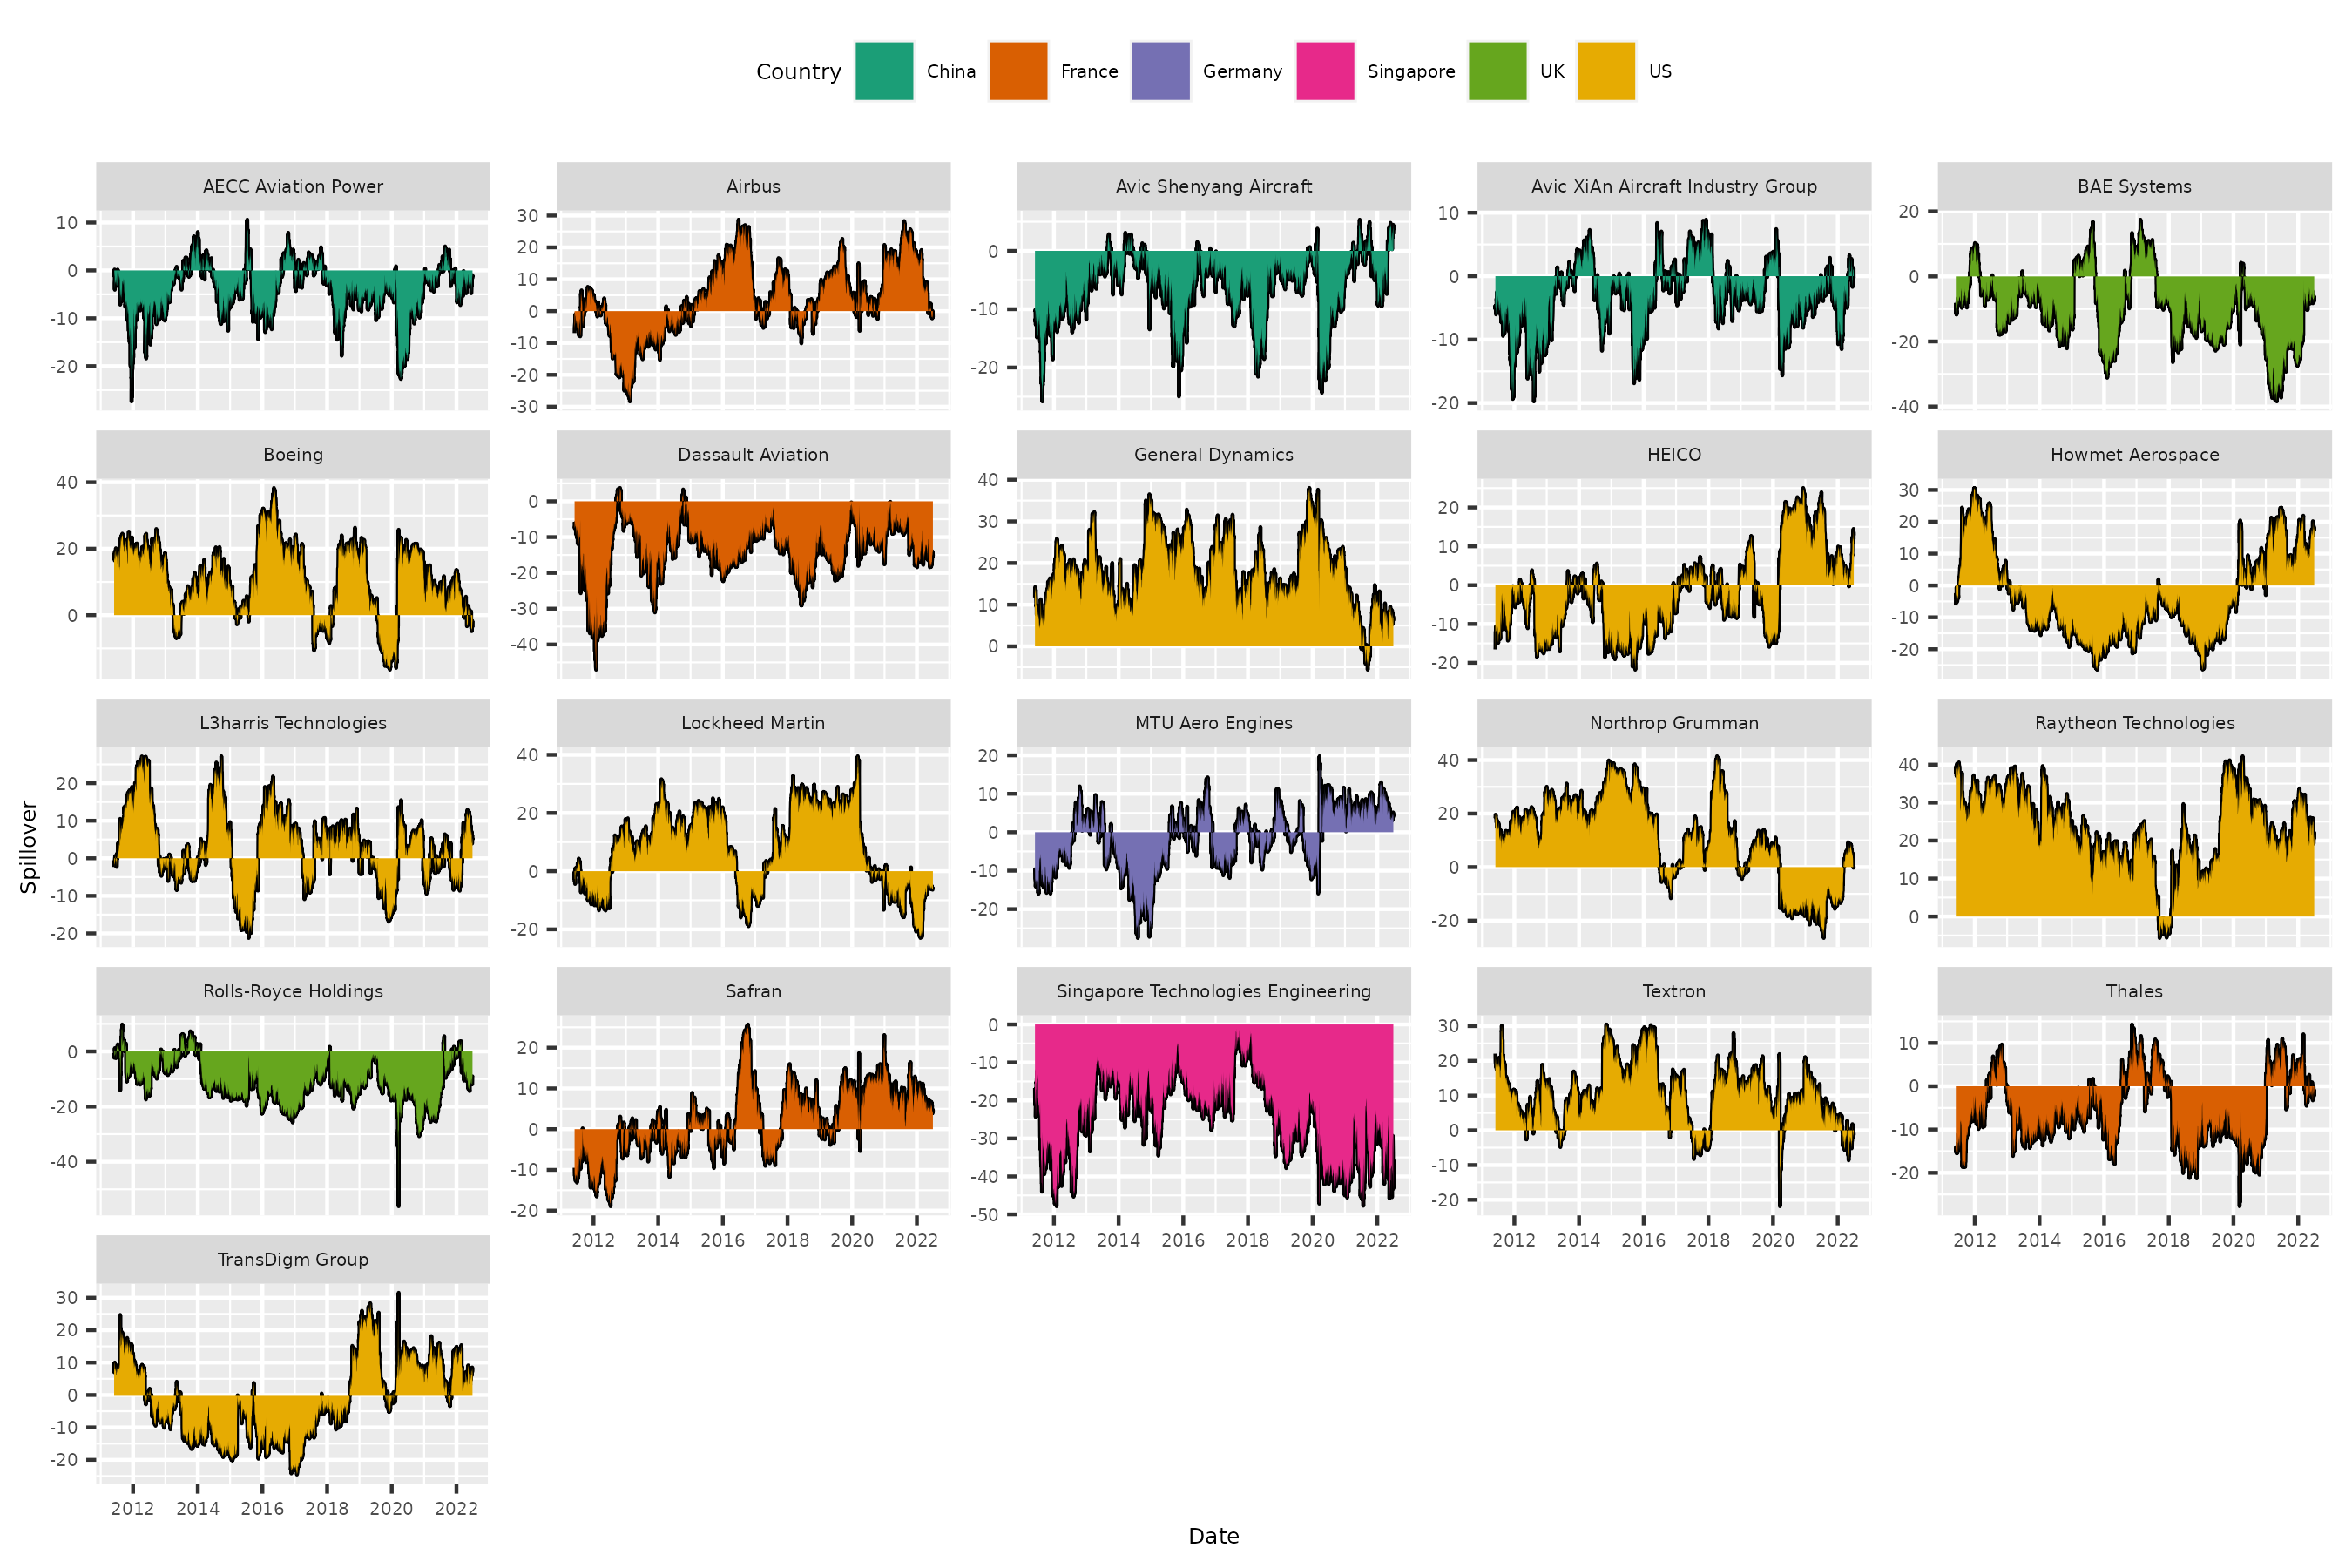
\includegraphics{plots/fig-rtnnet50.png}
  \caption{Net spillover effects for the stock returns at middle quantile (50th Percentile)}
  \label{fig:netrtn50}
\end{sidewaysfigure}

\begin{sidewaysfigure}
\centering
  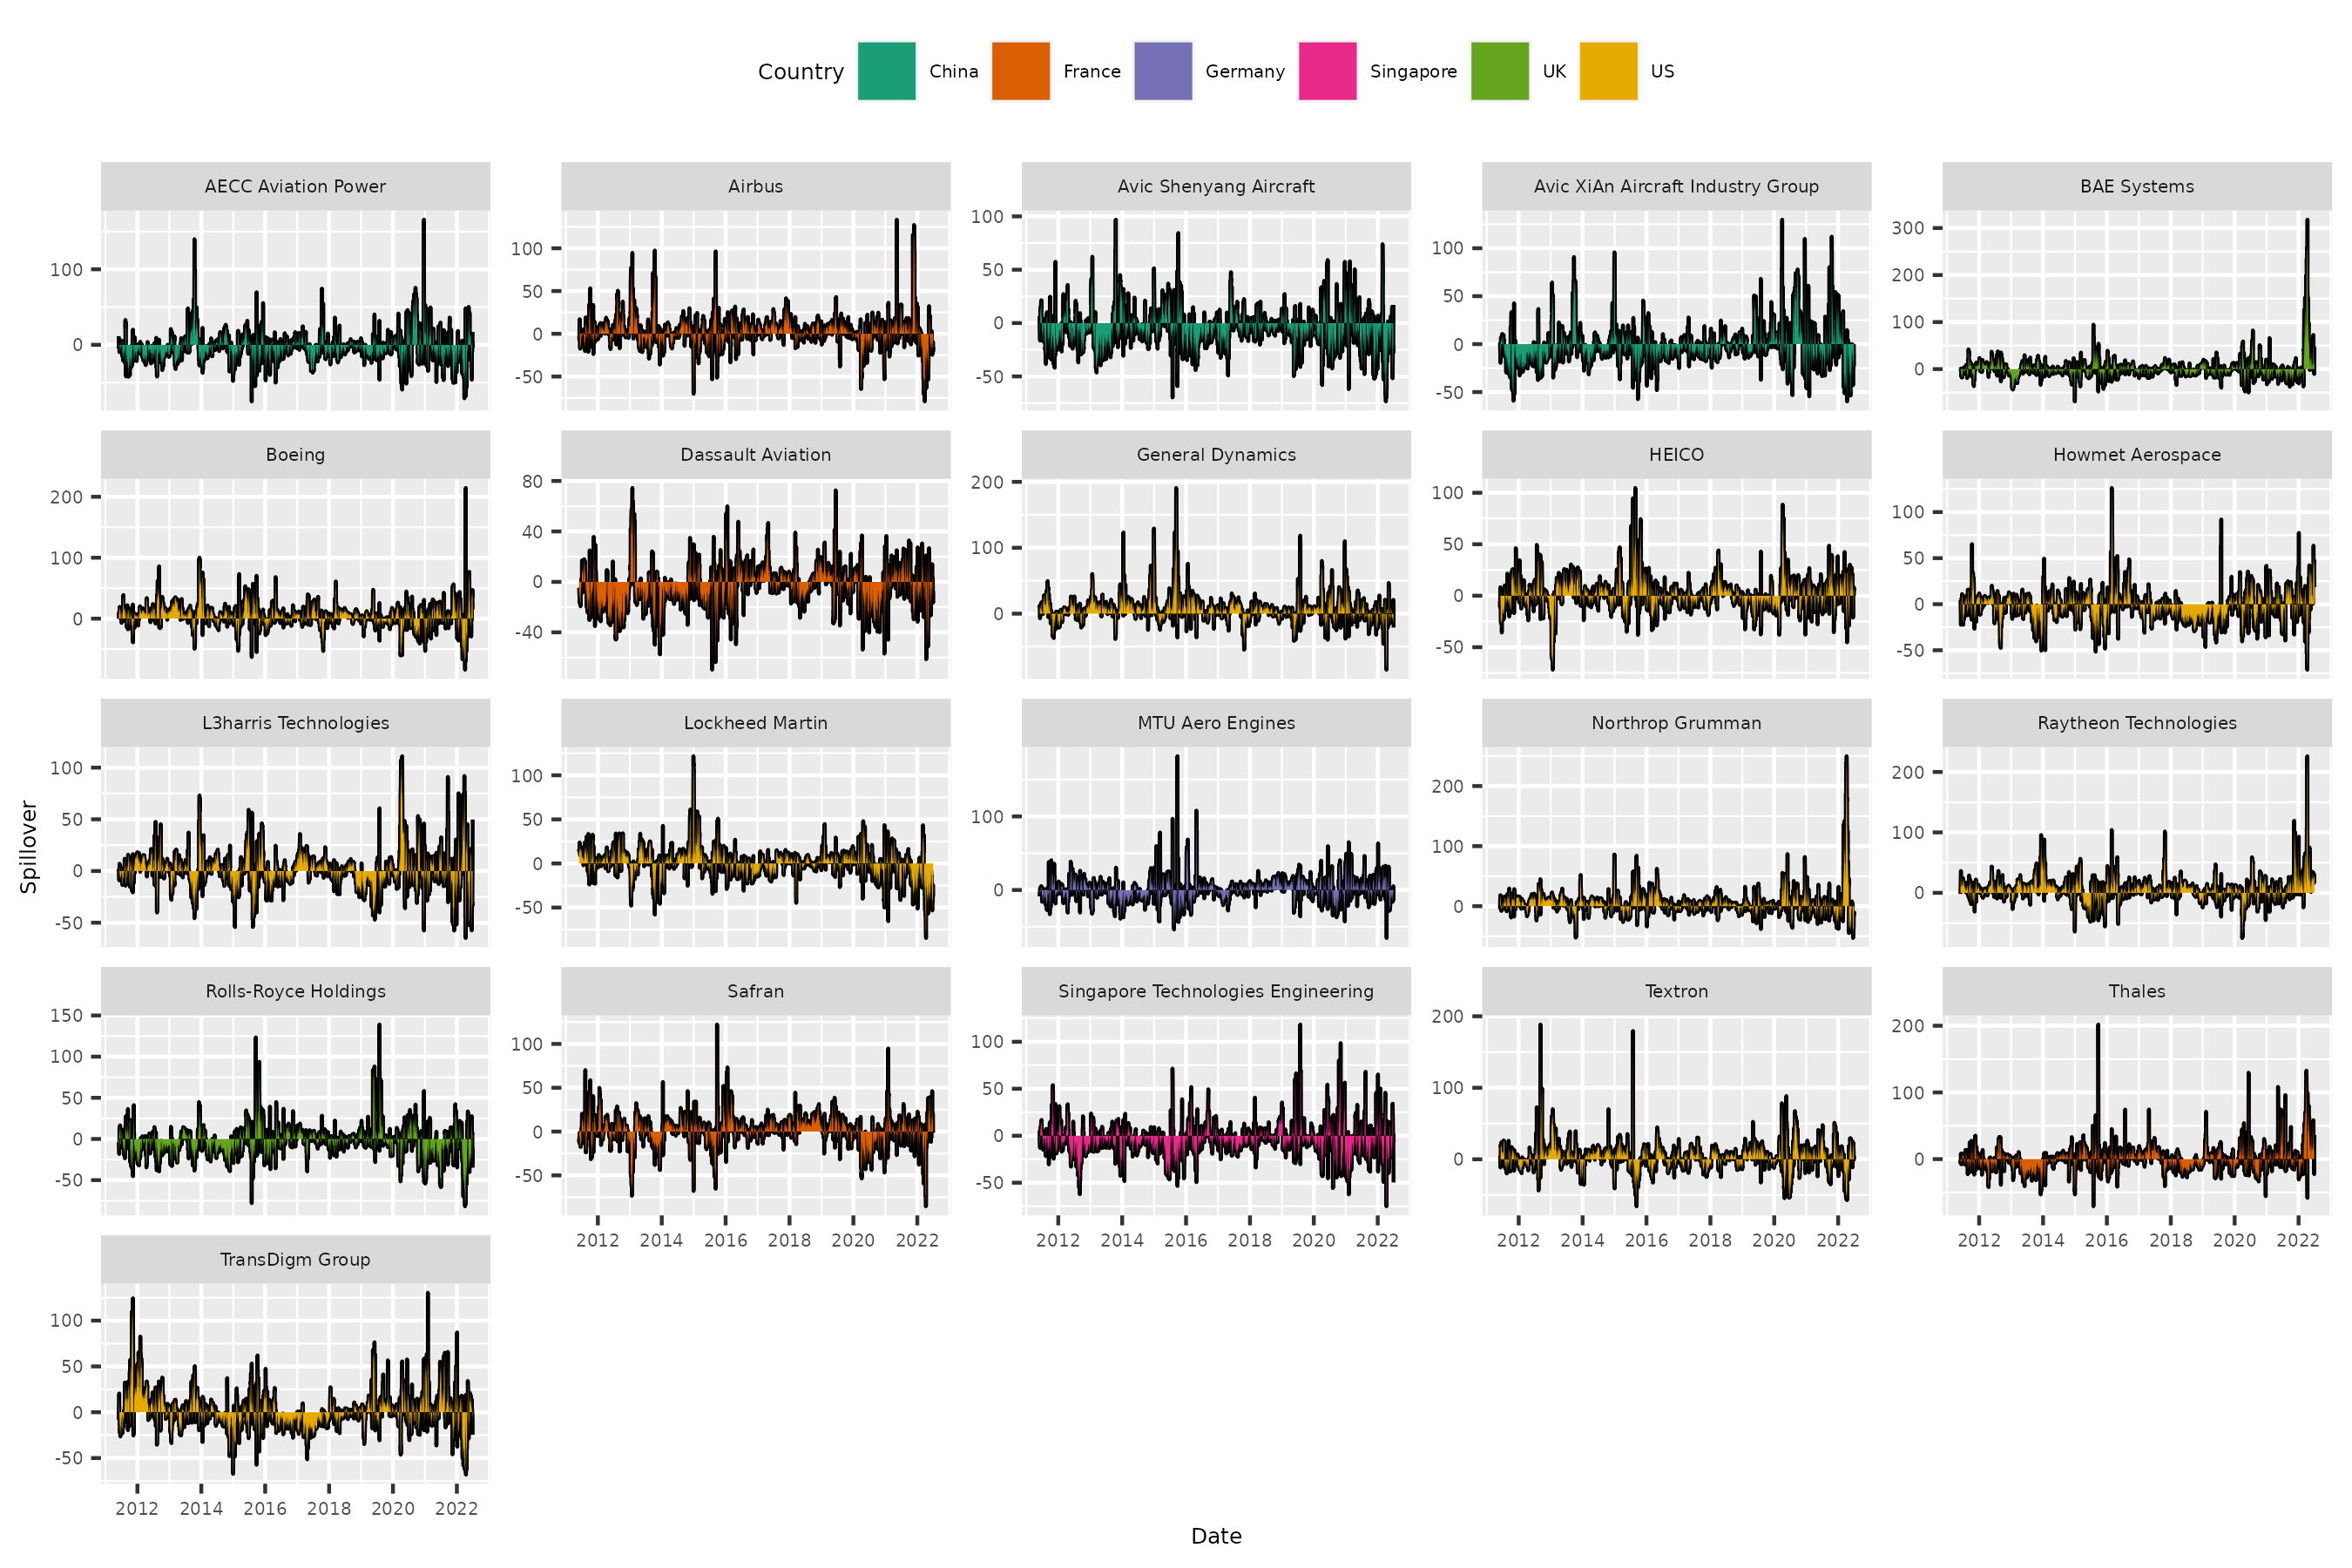
\includegraphics{plots/fig-rtnnet95.png}
  \caption{Net spillover effects for the stock returns at middle quantile (95th Percentile)}
  \label{fig:netrtn95}
\end{sidewaysfigure}

\begin{sidewaysfigure}
\centering
  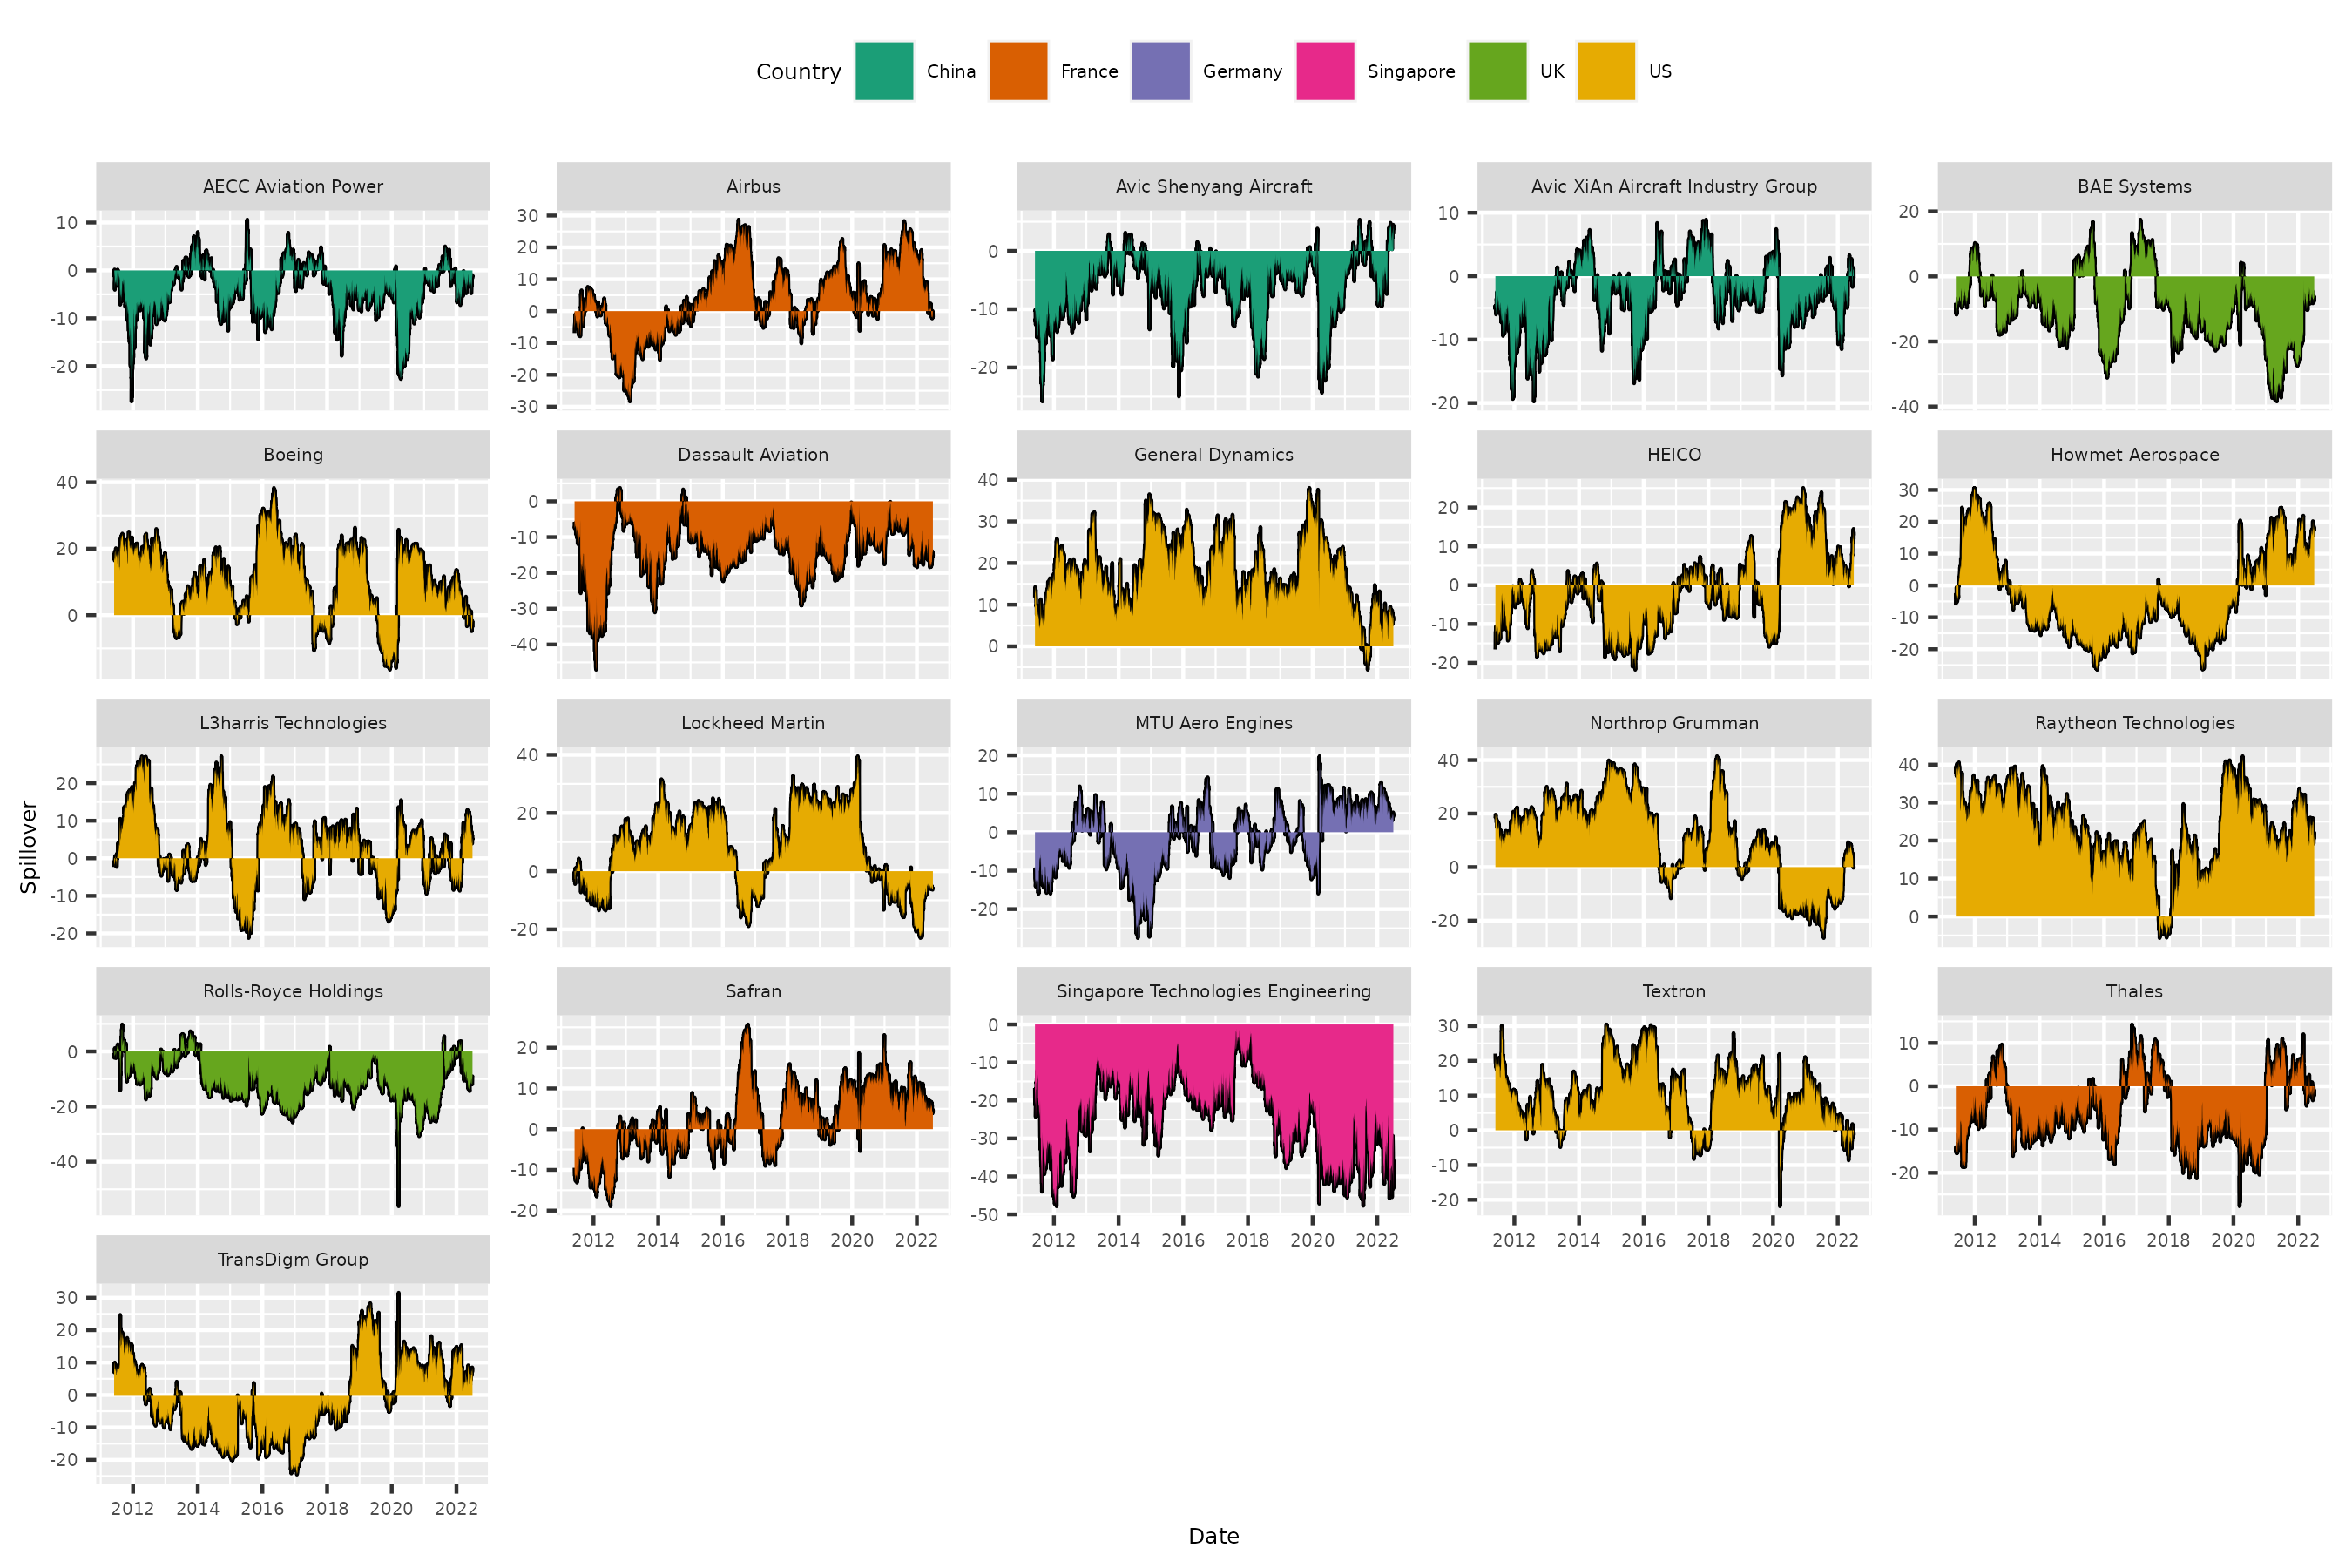
\includegraphics{plots/fig-rtnnet5.png}
  \caption{Net spillover effects for the stock returns at middle quantile (5th Percentile)}
  \label{fig:netrtnfive}
\end{sidewaysfigure}

We group these plots by country, and some interesting patterns emerge.
Firstly, at the median of distributions, the three Chinese defence
stocks are net spillover receivers in both their return performance and
volatility. This may indicate the need for global maturity in these
stocks compared to the other members of the system belonging to
developed markets (e.g., the US and Europe). Secondly, the US A\&D
stocks dominate the sample and are net transmitters of both volatility
and return spillover effects. More precisely, in normal periods (i.e.the
median of the conditional distribution), Raytheon Technologies and
General Dynamics are dominant net transmitters. This pattern also
replicates at the extremes of the conditional distributions. While this
is unsurprising given that Raytheon Technologies is the largest global
defence stock, it is worth noting that General Dynamics is the sixth
largest. For the latter, the result can be driven by some sizeable
recent defence contracts signed, for example, the US National
Geospatial-Intelligence Agency in March 2022 (US\$4.5 billion), the US
Navy in August 2022 (US\$1.4 billion) and the US Army in 2022 (US\$1.2
billion). Compared to the system of returns, the system of volatilities
exhibits much more time variation, perhaps indicative of the high
sensitivity to market fluctuations of financial risk.

\begin{sidewaysfigure}
\centering
  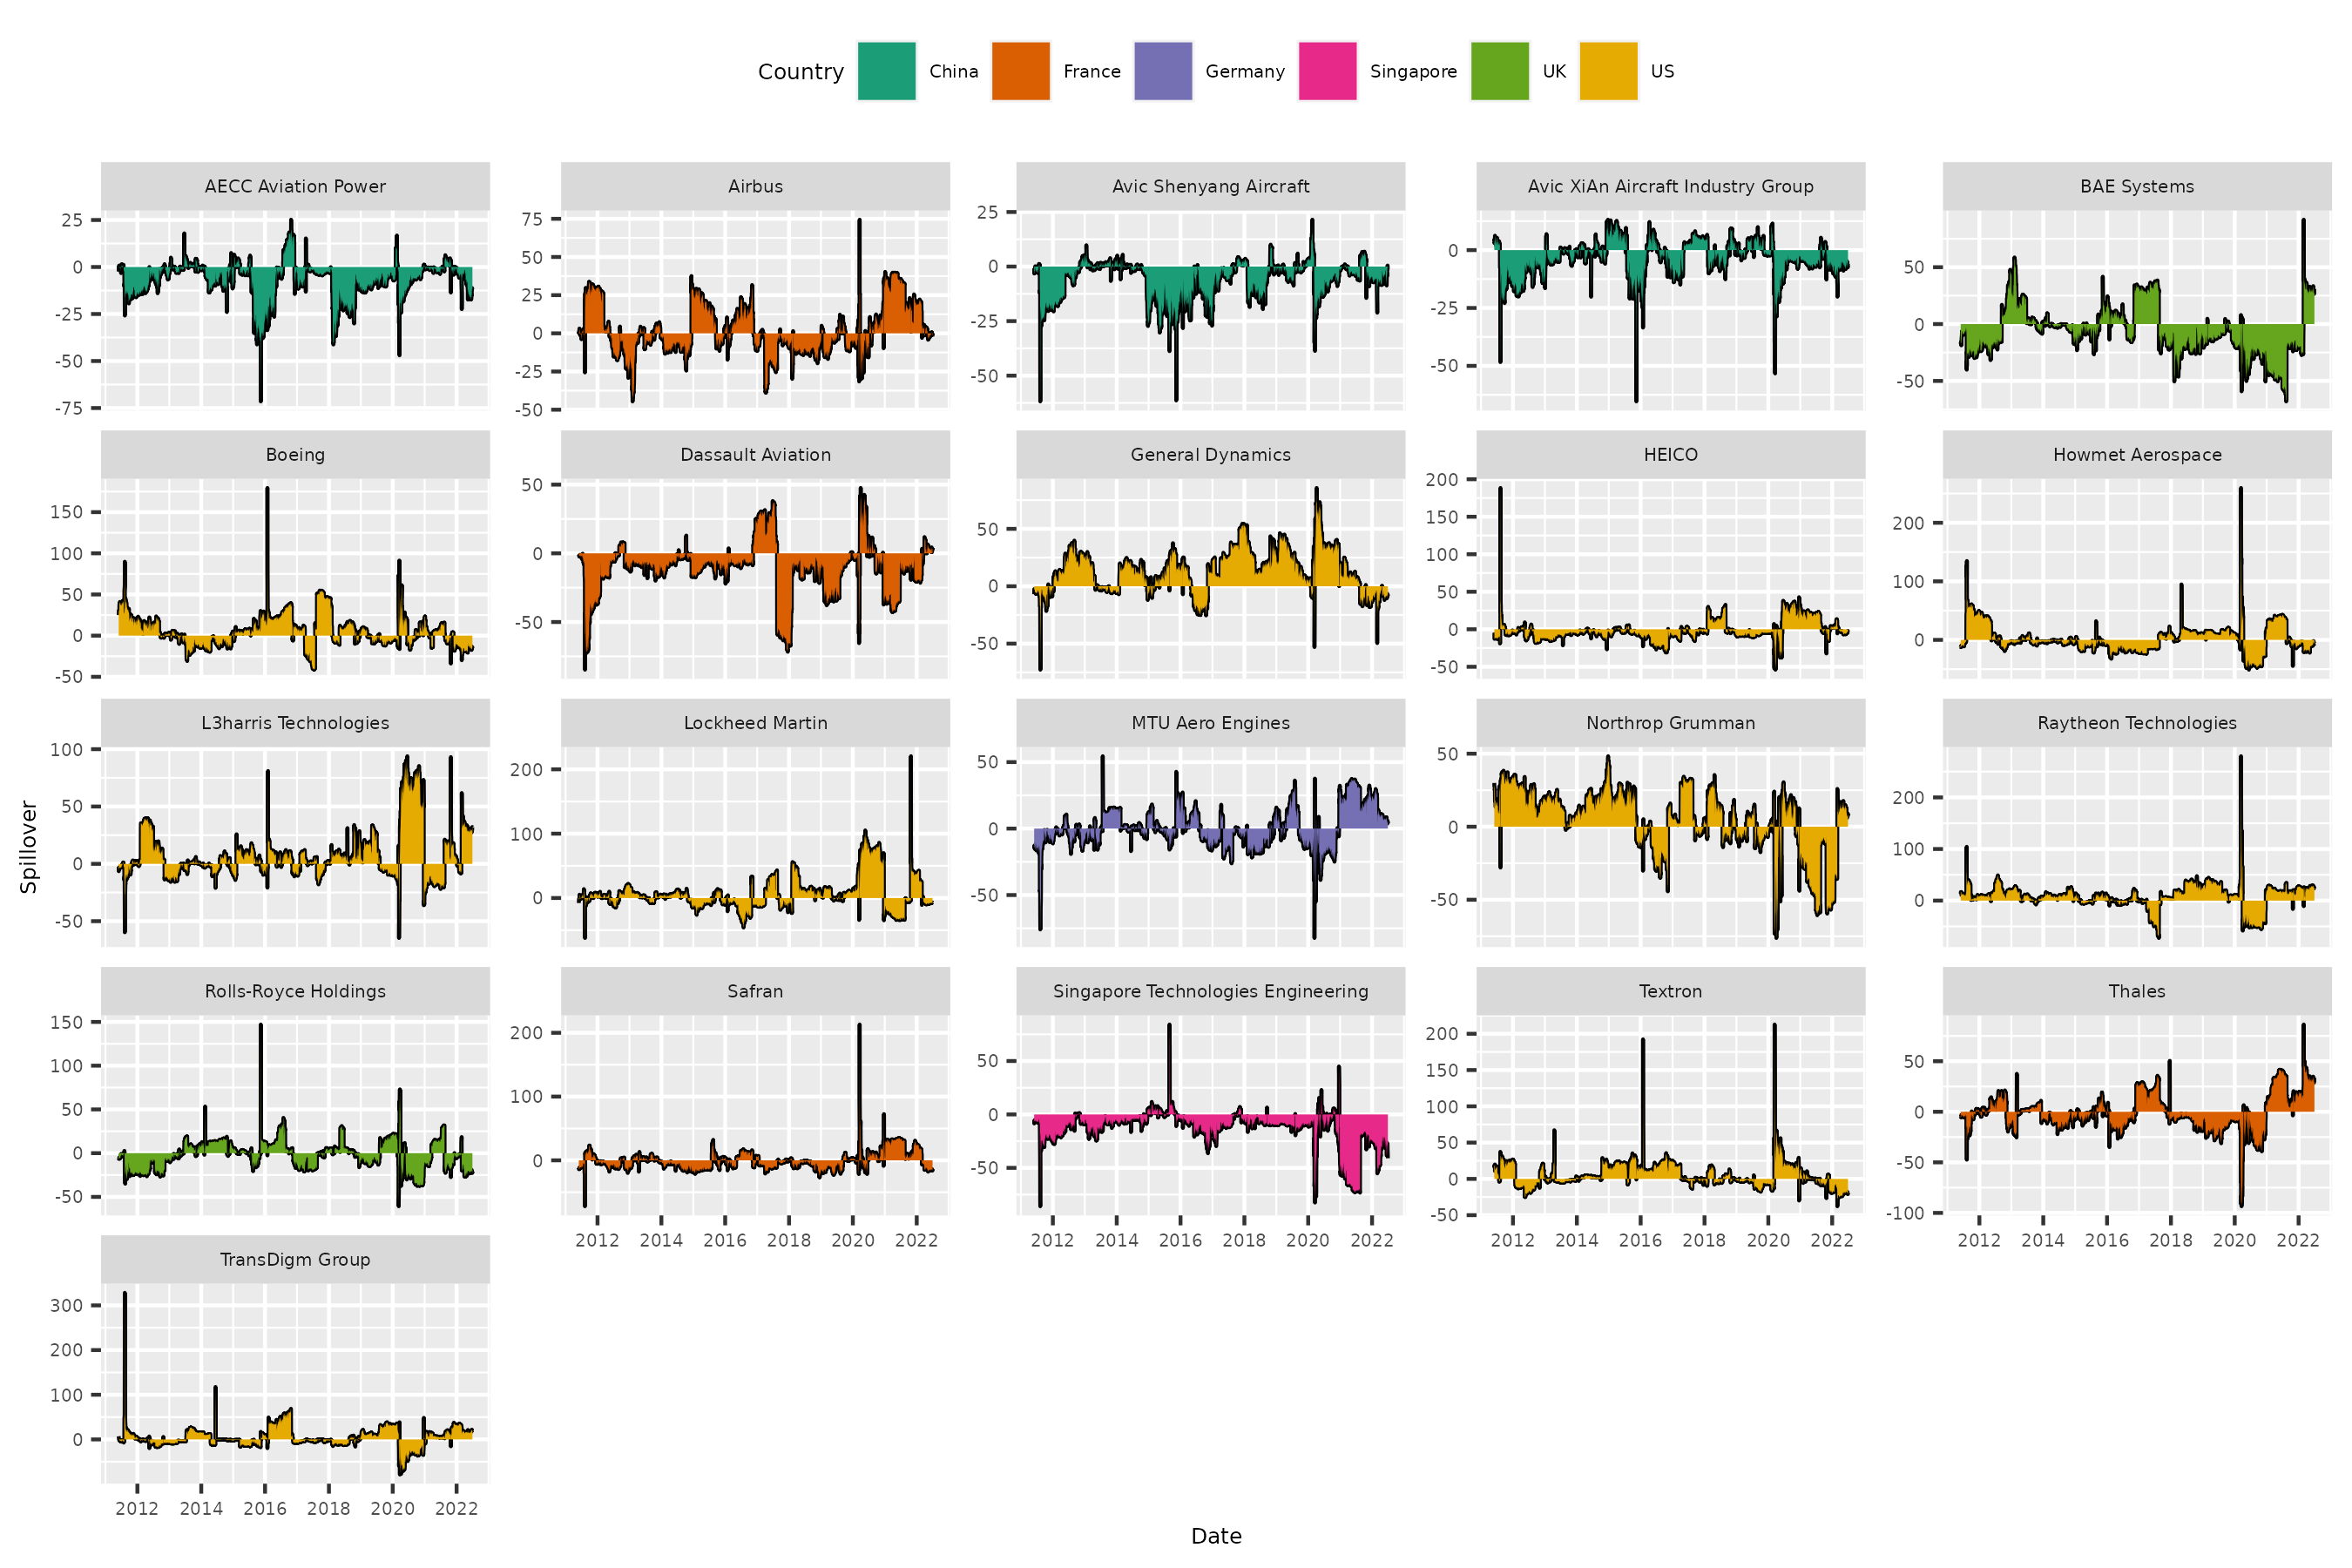
\includegraphics{plots/fig-volnet50.png}
  \caption{Net spillover effects for the stock volatilities at middle quantile (50th Percentile)}
  \label{fig:volnet50}
\end{sidewaysfigure}

\begin{sidewaysfigure}
\centering
  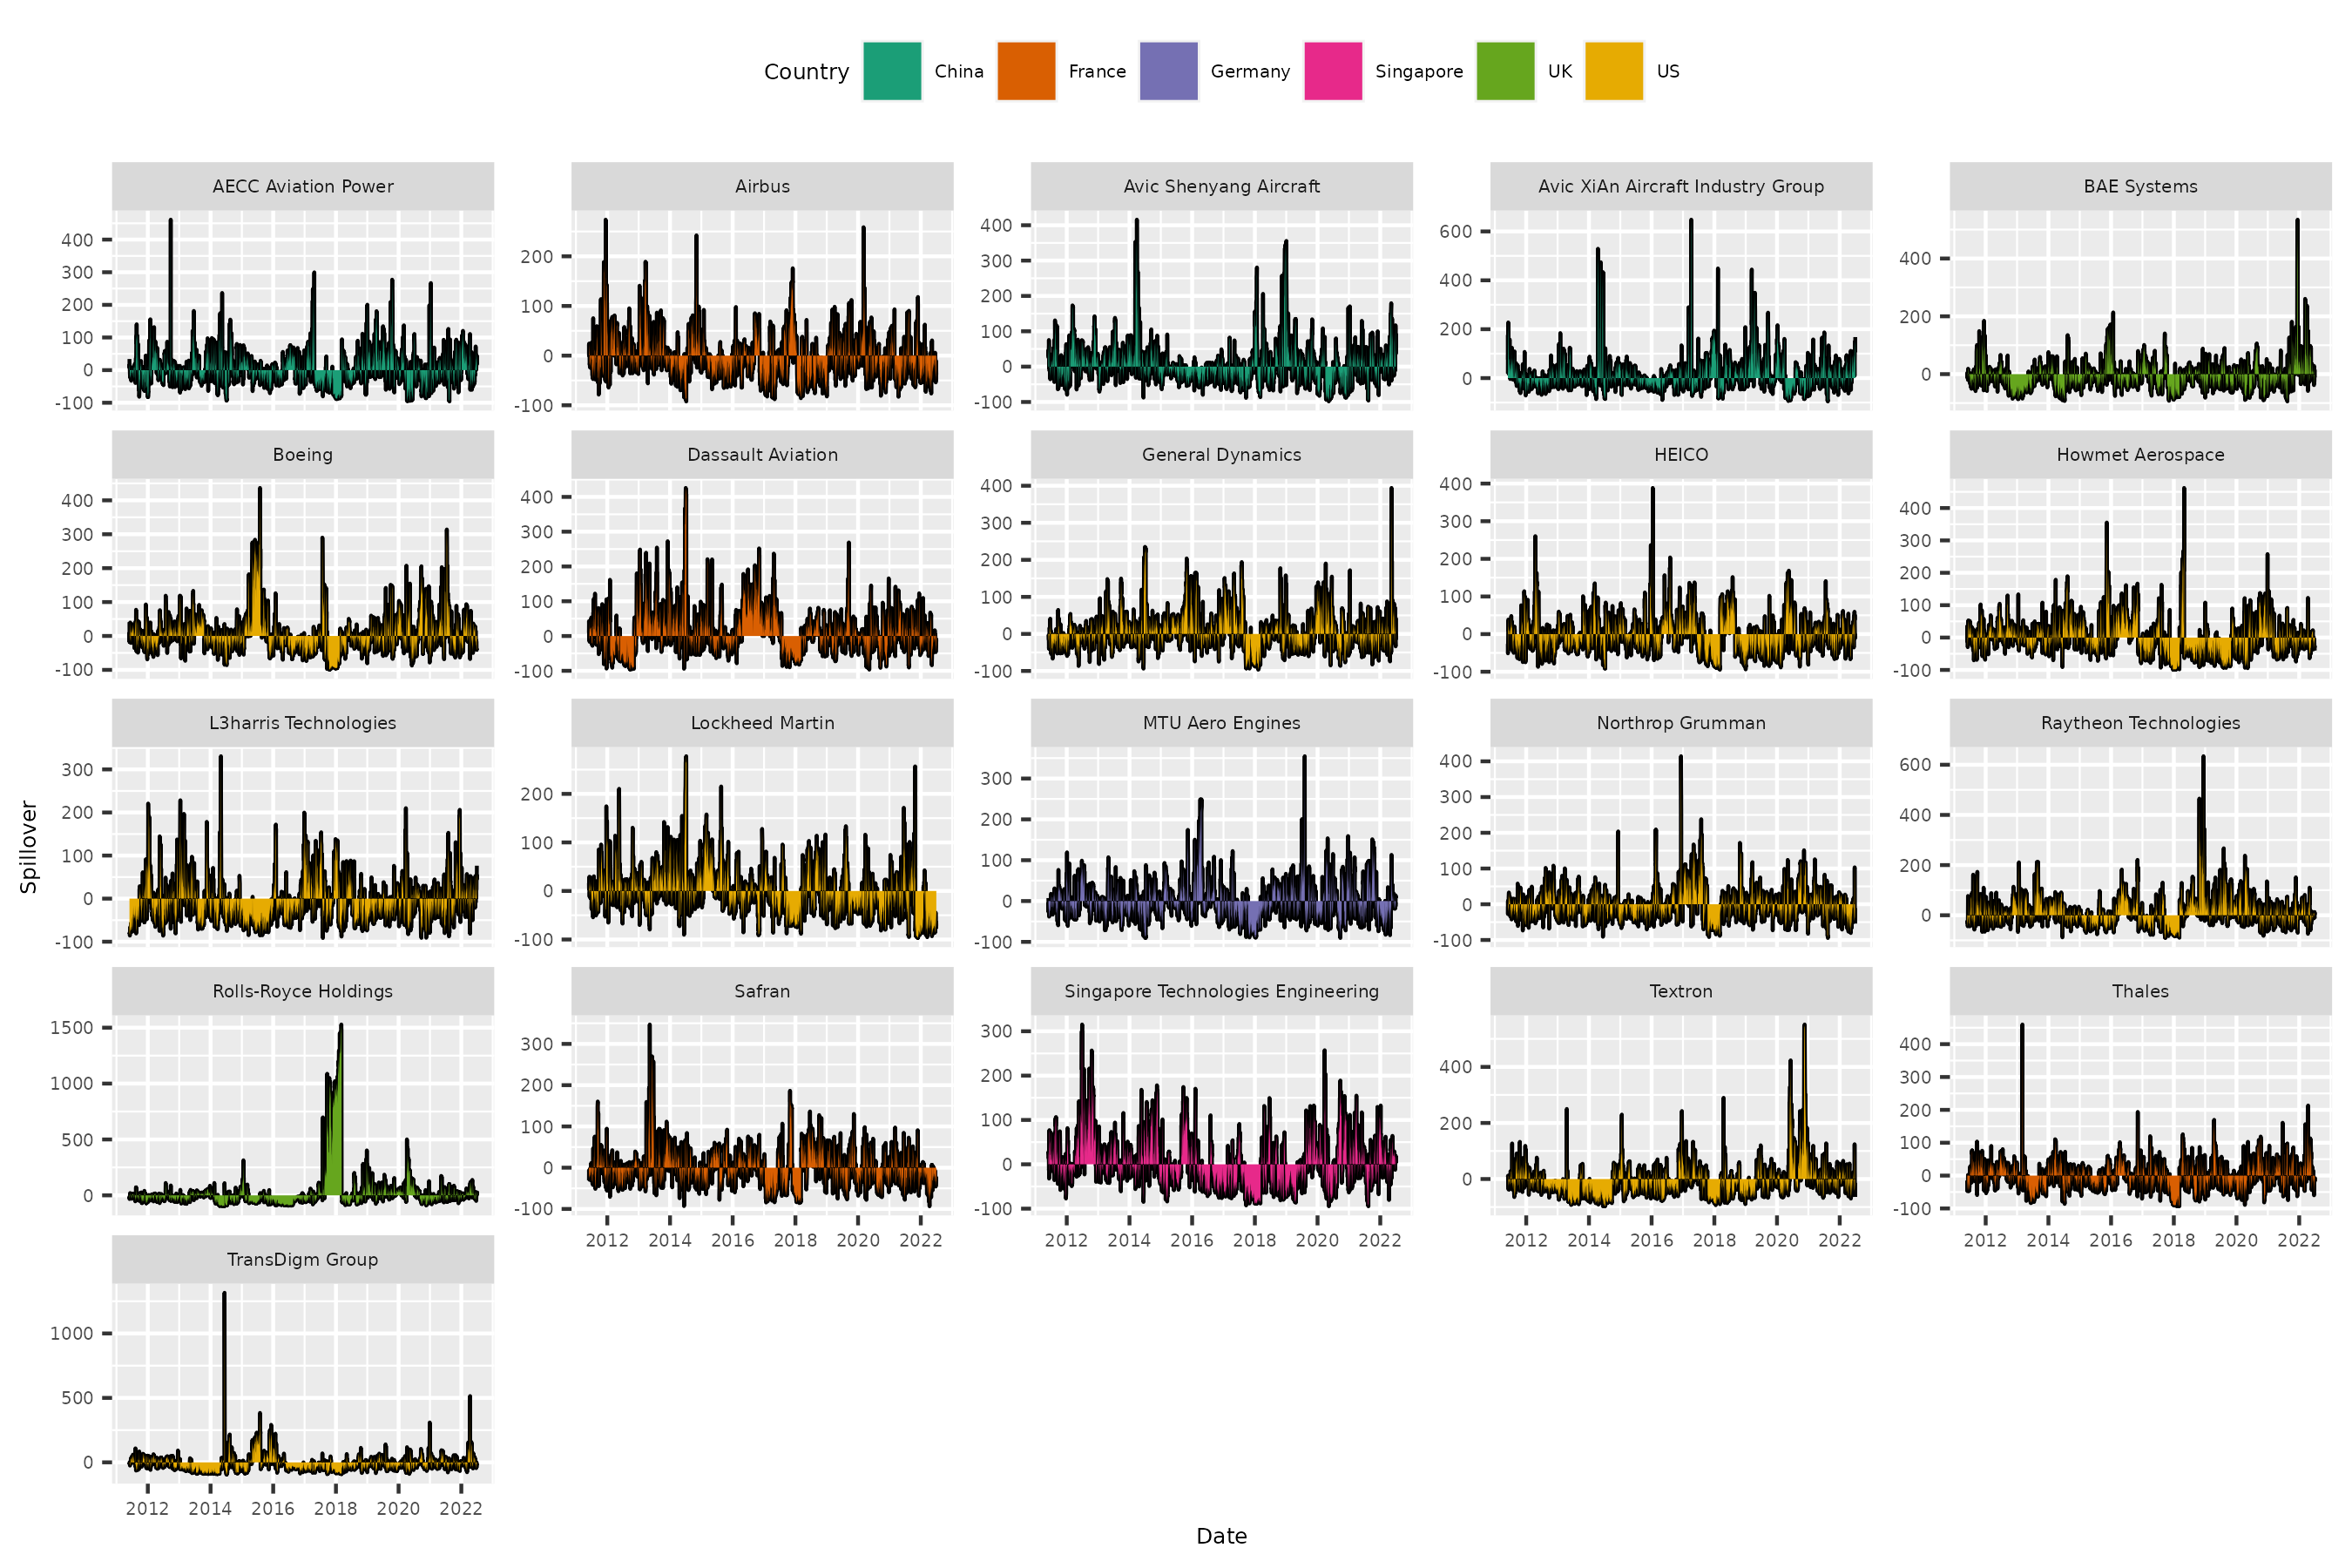
\includegraphics{plots/fig-volnet95.png}
  \caption{Net spillover effects for the stock volatilities at middle quantile (95th Percentile)}
  \label{fig:volnet95}
\end{sidewaysfigure}

\begin{sidewaysfigure}
\centering
  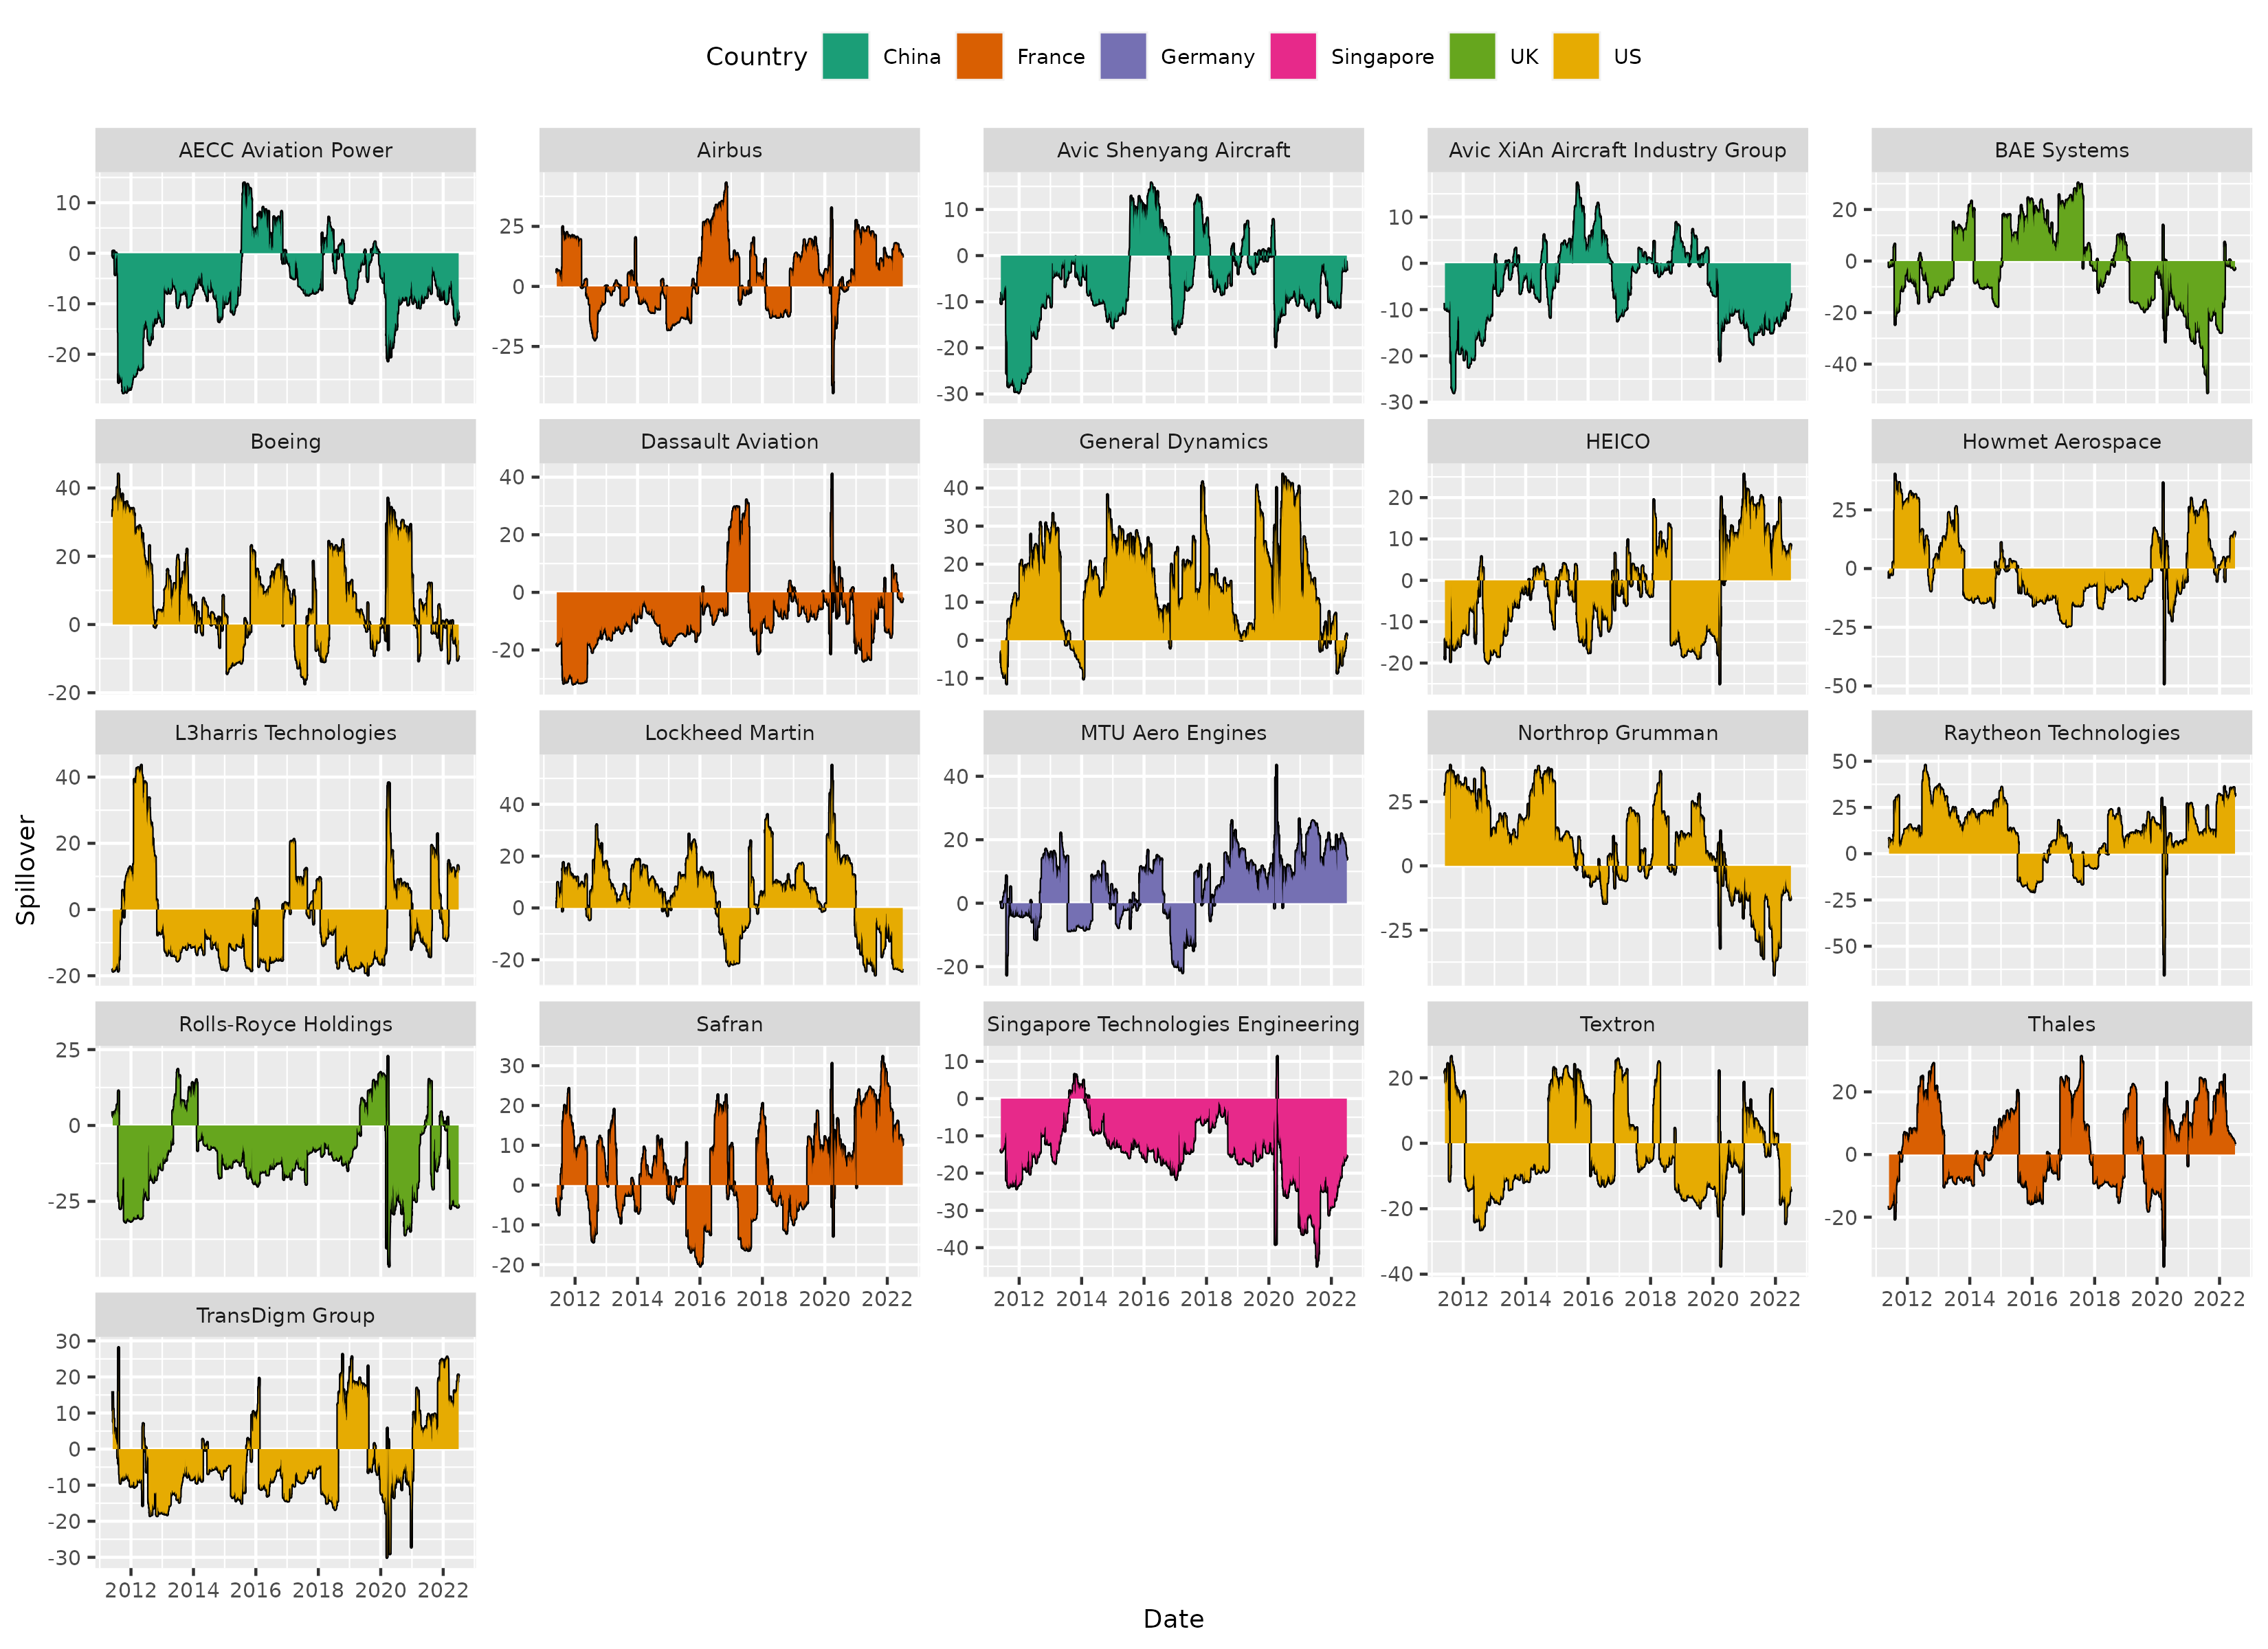
\includegraphics{plots/fig-volnet5.png}
  \caption{Net spillover effects for the stock volatilities at middle quantile (5th Percentile)}
  \label{fig:volnet5}
\end{sidewaysfigure}

In terms of the prominent dates in Figure \ref{fig:volnet50}, Figure
\ref{fig:volnet95}, and Figure \ref{fig:volnet5} there are notable
positive spikes at the start of the COVID-19 pandemic with the largest
appearing in the median of the conditional distribution of the
volatility system. The largest of these are in Raytheon Technologies and
Howmet Aerospace, which both spike at over 200 in net transmission
terms. Within the US stocks, Raytheon and General Dynamics are the most
transmitive in both their median and extreme spillover effects. Finally,
in terms of magnitude, Singapore technology engineering, are the largest
receiver of spillover effects at both the median and the extremes, which
is not surprising given their small market capitalization compared to
the others (see Table~\ref{tbl-A1} for details of size of stocks).

Compared to previous studies, our above findings reveal that both return
and volatility spillovers are unstable over time, and those estimated at
normal market conditions (at the middle quantile), intensify during
crisis periods such as the COVID-19 outbreak. There is also evidence of
intensified spillover effects for return shocks at both lower and upper
quantiles, exceeding the return spillover effects estimated at the
middle quantile, thus indicating significantly different behaviour of
spillovers across different market conditions. The level of spillovers
at the lower quantile in the return system is considerably larger than
that in the volatility system. However, the level of volatility
spillover is exceptionally high at the upper quantile only and exhibits
a low variability. Finally, Chinese defence stocks seem segmented from
the rest under normal return conditions and a moderate volatility state.
However, they somewhat integrated with global defence stocks under
extreme return conditions and volatility states. This implies that
Chinese defence stocks entail more diversification benefits under normal
conditions than bear or bull markets when returns and volatility are
very low or high.

\hypertarget{drivers-of-return-and-spillovers-the-role-of-geopolitical-risk}{%
\subsection{Drivers of return and spillovers -- the role of geopolitical
risk}\label{drivers-of-return-and-spillovers-the-role-of-geopolitical-risk}}

In this section, we provide insights into the main drivers of return and
volatility spillovers across A\&D stocks while paying particular
attention to the impact of geopolitical risk. The explanatory variables
considered in the analysis, selected based on previous studies, are:

\begin{itemize}
\tightlist
\item
  The geopolitical risk (GPR) index of Caldara and Iacoviello (2022),
  which is constructed based on press articles covering 11 leading
  international newspapers, and defined as ``the kind of risk related to
  events such as wars, terrorist acts and political tensions, that can
  affect the normal and peaceful process of international relations''
  (Caldara and Iacoviello, 2022)\footnote{We ensure that all variables
    entered in the regression are stationary, whether in their original
    levels or transformed (e.g.~change) levels.};
\item
  An interaction of GPR with the COVID-19 pandemic and Russian-Ukraine
  war (), where is a dummy variable taking the value of 1 during the
  COVID-19 outbreak and war period (January 02, 2020-- July 01, 2022)
  and 0 otherwise;
\item
  The US economic policy uncertainty (US EPU) index of Baker et
  al.~(2016), constructed based on US newspaper articles reflecting
  uncertainties in US economic policies;
\item
  The CBOE VIX index, which captures the 30-day expected volatility of
  the US stock market and is often used a proxy of fear among investors,
  not only in the US but across the global stock markets;
\item
  The log returns on the S\&P 500 Composite Index, which is used as a
  proxy for the performance of the global stock markets;
\item
  The US Treasury spread, computed as ``10-Year Treasury Constant
  Maturity Minus 2-Year Treasury Constant Maturity'', which reflects the
  shape of the US yield curve;
\item
  The TED spread, computed as the 3-month LIBOR USD rate minus the
  3-month US Treasury Bill rate, which captures short-term liquidity
  risk;
\item
  Default spread, computed as the yield on Moody's BAA-rated bonds minus
  the yield on AAA-rated corporate bonds, reflecting corporate credit
  conditions;
\item
  US business conditions, measured by the Aruoba-Diebold-Scotti (ADS)
  index of Aruoba et al.~(2009), which measures real business conditions
  on a daily basis;
\item
  The US inflation expectation, as measured by the 5-Year Breakeven
  Inflation Rate (T5YIE);
\end{itemize}

We report the estimated coefficients of Equation~\ref{eq-reg} in
Table~\ref{tbl-reg1} for return spillovers and in Table~\ref{tbl-reg2}
for volatility spillovers\footnote{We ensure that all variables entered
  in the regression are stationary, whether in their original levels or
  transformed (e.g.~change) levels.}

\begin{equation}\protect\hypertarget{eq-reg}{}{TOTAL_t=c+b_1GPR_{t-1}+b_2GPR_{t-1}.DCOVID+b_{it}X_{t-1}+e_t}\label{eq-reg}\end{equation}

where \(TOTAL_t\) is the total spillover index in the system of return
or volatility across A\&D companies, estimated at the lower, middle, or
higher quantiles; \(GPR\_{t-1}\) is the lagged value of the geopolitical
risk; \(GPR_{t-1}.DCOVID\) is the interaction term between GPR and the
COVID-19 and Russian-Ukraine war period; \(X_{t-1}\) is the vector of
the lagged value of control variables, described above, and is the
residual term. Except for GPR index\footnote{GPR data are downloaded
  from https://www.matteoiacoviello.com/gpr.htm.}, data on the other
explanatory variables are collected from Refinitiv.

\hypertarget{tbl-reg1}{}
\begin{table}[H]
\caption{\label{tbl-reg1}Drivers of return spillovers across A\&D companies for the full sample
period }\tabularnewline

\centering
\resizebox{\linewidth}{!}{
\begin{tabular}[t]{lllllll}
\toprule
\multicolumn{1}{c}{ } & \multicolumn{2}{c}{Middle quantile} & \multicolumn{2}{c}{Upper quantile} & \multicolumn{2}{c}{Lower quantile} \\
\cmidrule(l{3pt}r{3pt}){2-3} \cmidrule(l{3pt}r{3pt}){4-5} \cmidrule(l{3pt}r{3pt}){6-7}
Variable & Coefficient & Prob. & Coefficient & Prob. & Coefficient & Prob.\\
\midrule
GPRD(-1) & -0.033 & 0.000 & -0.003 & 0.000 & -0.003 & 0.000\\
GPRD(-1)*DCOVID & 0.069 & 0.000 & 0.007 & 0.000 & 0.006 & 0.000\\
USEPU(-1) & 0.008 & 0.004 & 0.001 & 0.040 & 0.001 & 0.048\\
VIX(-1) & 0.164 & 0.004 & 0.011 & 0.062 & 0.028 & 0.000\\
SP500(-1) & 24.392 & 0.027 & 0.075 & 0.957 & 6.462 & 0.000\\
\addlinespace
TERM SPREAD(-1) & -0.733 & 0.809 & 0.470 & 0.269 & -0.463 & 0.300\\
TED SPREAD (-1) & -0.079 & 0.000 & -0.005 & 0.002 & -0.003 & 0.122\\
DEFAULT SPREAD(-1) & 19.867 & 0.000 & 1.401 & 0.000 & 0.683 & 0.001\\
ADS BUS CONDITION INDEX(-1) & 0.713 & 0.000 & 0.071 & 0.000 & 0.066 & 0.000\\
US INFLATION(-1) & 2.478 & 0.001 & 0.122 & 0.134 & -0.474 & 0.000\\
\addlinespace
C & 42.044 & 0.000 & 91.401 & 0.000 & 92.879 & 0.000\\
 &  &  &  &  &  & \\
Adjusted R-squared & 0.640 &  & 0.392 &  & 0.387 & \\
F-statistic & 468.741 &  & 170.260 &  & 166.738 & \\
Prob(F-statistic) & 0.000 &  & 0.000 &  & 0.000 & \\
\bottomrule
\multicolumn{7}{l}{\textsuperscript{} Notes: This table presents the estimated coefficients of the regression model in}\\
\multicolumn{7}{l}{Equation (6) based on a covariance estimator that accounts for the presence of}\\
\multicolumn{7}{l}{heteroscedasticityand autocorrelation (HAC). The sample period is 23 August 2010 –July}\\
\multicolumn{7}{l}{1, 2022.}\\
\end{tabular}}
\end{table}

\hypertarget{tbl-reg2}{}
\begin{table}[H]
\caption{\label{tbl-reg2}Drivers of volatility spillovers across A\&D companies for the full
sample period }\tabularnewline

\centering
\resizebox{\linewidth}{!}{
\begin{tabular}[t]{lllllll}
\toprule
\multicolumn{1}{c}{ } & \multicolumn{2}{c}{Middle quantile} & \multicolumn{2}{c}{Upper quantile} & \multicolumn{2}{c}{Lower quantile} \\
\cmidrule(l{3pt}r{3pt}){2-3} \cmidrule(l{3pt}r{3pt}){4-5} \cmidrule(l{3pt}r{3pt}){6-7}
Variable & Coefficient & Prob. & Coefficient & Prob. & Coefficient & Prob.\\
\midrule
GPRD(-1) & -0.061 & 0.000 & -0.002 & 0.040 & -0.042 & 0.000\\
GPRD(-1)*DCOVID & 0.115 & 0.000 & 0.001 & 0.194 & 0.072 & 0.000\\
USEPU(-1) & 0.035 & 0.000 & 0.000 & 0.257 & 0.014 & 0.000\\
VIX(-1) & 0.499 & 0.000 & 0.000 & 0.933 & 0.416 & 0.000\\
SP500(-1) & 84.600 & 0.000 & -1.099 & 0.419 & 61.075 & 0.000\\
\addlinespace
TERM SPREAD(-1) & -7.221 & 0.204 & -1.217 & 0.004 & -6.611 & 0.089\\
TED SPREAD (-1) & -0.019 & 0.482 & 0.000 & 0.923 & -0.055 & 0.003\\
CORPORATE CREDIT CONDITIONS(-1) & 14.191 & 0.000 & 0.060 & 0.695 & 16.357 & 0.000\\
ADS\_BUS\_CONDITION\_INDEX(-1) & 1.001 & 0.000 & 0.001 & 0.884 & 0.686 & 0.000\\
US INFLATION(-1) & 3.410 & 0.017 & -0.034 & 0.602 & 4.760 & 0.000\\
\addlinespace
C & 23.931 & 0.000 & 94.961 & 0.000 & 33.540 & 0.000\\
 &  &  &  &  &  & \\
Adjusted R-squared & 0.584 &  & 0.012 &  & 0.613 & \\
F-statistic & 369.986 &  & 4.247 &  & 416.551 & \\
Prob.(F-statistic) & 0.000 &  & 0.000 &  & 0.000 & \\
\bottomrule
\multicolumn{7}{l}{\textsuperscript{} Notes: This table presents the estimated coefficients of the regression model in Equation (7)}\\
\multicolumn{7}{l}{based on a covariance estimator that accounts for the presence of heteroscedasticityand}\\
\multicolumn{7}{l}{autocorrelation (HAC). The sample period is 23 August 2010 –July 1, 2022.}\\
\end{tabular}}
\end{table}

Starting with the drivers of the TCI of returns, Table~\ref{tbl-reg1}
shows that many of the estimated coefficients of explanatory variables
are not necessarily the same across the middle and upper/lower quantile
spillovers. However, the GPR index is a significant driver of return
spillovers at all quantiles, and its effect is positive and significant
for all cases after controlling for the COVID-19 outbreak period, which
includes the Russian-Ukraine war sub-period. This suggests that the
heightened level of geopolitical risk around the war period has led to
increased return spillovers across A\&D stocks. Regarding the control
variables, we notice that S\&P500 returns, VIX, default spread, and
business conditions positively impact return spillovers, irrespective of
the quantile, bearing in mind that their magnitude is the largest at the
middle quantile. Table~\ref{tbl-reg2} considers the results on the
drivers of volatility spillovers. The results point to the exact impact
of GPR on volatility spillovers, especially when the interaction term is
considered, except at the upper quantile. Among the other explanatory
variables, we highlight the significant role played by corporate credit
conditions, stock market volatility, short-term liquidity risk, and
real-time business conditions.

Furthermore, we conduct a robustness analysis using the GPRACT sub-index
instead of the GPR index while estimating Equation (6). Given that our
analysis covers the war in Ukraine period, the use of the GPRACT
dimension of the GPR index is very crucial because it reflects the
realization of adverse events and war-related events and military acts
unlike the GPRTHREAT dimension which only reflects geopolitical tensions
and military threats (Caldara and Iacoviello 2022) . The results from
the re-estimation of Equation (6) using GPRACT instead of GPR are
presented in Appendix Tables A4 and A5. They are quite similar to those
reported in Tables 4 and 5, which confirms the role of geopolitical
risks in driving the spillovers of returns and volatility among A\&D
stocks and thus the robustness of our results to the choice of the proxy
of geopolitical risk.

\hypertarget{conclusion}{%
\section{Conclusion}\label{conclusion}}

This study analyses the return and volatility connectedness of a sample
of major A\&D stocks in normal and extreme market periods using a
quantile-based VAR approach of connectedness, which captures the system
of connectedness at lower, middle, and upper parts of the conditional
distribution of both returns and volatility. Then, the drivers of the
connectedness index estimated across various quantiles are revealed,
notably the geopolitical risk index.

The main results suggest evidence of variation in the quantile structure
of the system of connectedness among major A\&D stocks. The network
topology analysis shows that shocks propagate more strongly at both
lower and upper tails of the conditional distribution than at the
conditional median, suggesting that the structure of spillovers at both
tails is dissimilar to that observed at the conditional median. However,
the magnitude of bilateral connections is smaller at the tails than at
the median, but they are more apparent. In the latter, connectedness is
stronger within countries, but the volatility and return systems are
less connected overall. Finally, we find that shocks are smaller and
disproportionately larger in US stocks when comparing bear market and
bull market conditions. These results suggest that the evolution of the
dependence structure at the tails is notable and should not be
overlooked. In other words, the system-wide connectedness of shocks in
the A\&D industry can be masked when connectedness measures are
estimated at the conditional median or mean, thus missing a significant
portion of the spillover information related to extraordinarily negative
and positive shocks and extremely low and high volatility states.
Accordingly, applying quantile-based models of connectedness is
recommended as a natural extension to the pervasive average-based
models. This finding result matters for asset pricing and allocation
under various market conditions.

The application of a time-varying analysis shows that the degree of
tail-dependence varies with time and intensifies during periods of
economic and geopolitical-conflict turmoil. Intuitively, the main
findings generally concord with the literature on the return and
volatility spillovers under various market conditions in the global
stock markets, which reflect the nature of A\&D stocks despite their
price outperformance during periods of intensified geopolitical risk.
Furthermore, the relative tail dependence calculation indicates an
asymmetry between the behaviour of return (volatility) spillovers in
lower and upper quantiles. The findings on the extreme connectedness at
upper and lower tails offer a nuanced view of the importance of tail
risk propagation within the network system of A\&D stocks, which points
to the utility of adopting quantile-based methods of spillovers to
differentiate between the networks of spillovers under various market
conditions. This might concern the supervision of risk under extreme
market conditions. In fact, by extending our knowledge regarding the
effects of the size and sign of the spillovers on the system of
connectedness among significant A\&D stocks, policymakers can use
appropriate policy tools and surveillance mechanisms to manage potential
adversative impacts from extreme risk spillovers in the A\&D industry.

Additional analysis reveals the importance of geopolitical risk at the
end of the sample period in driving the spillovers of both returns and
volatility without underestimating the significant role played by some
macroeconomic and financial variables. Therefore, market participants
should closely examine the geopolitical risk levels for making
inferences on market integration in the aerospace and defence industry
and the diversification possibilities across various market conditions.

Our analysis is not free of limitations. Given that the GPR index and
its sub-indices are text-based indices,newspaper articles generally
follow events; therefore, the stock markets, especially in developed
economies, respond much quicker to (geopolitical) events than
newspapers. This would lead to possible endogeneity issues with the GPR
\footnote{We thank the reviewer for pointing to this issue.}, which
require more a refined consideration and analysis that shouldbe the
subject of future related studies.

\hypertarget{appendix}{%
\section{Appendix}\label{appendix}}

\setcounter{table}{0}
\renewcommand{\thetable}{A\arabic{table}}

\hypertarget{tbl-A1}{}
\begin{table}[H]
\caption{\label{tbl-A1}Size information for our study's sample }\tabularnewline

\centering
\resizebox{\linewidth}{!}{
\begin{tabular}[t]{lrrr}
\toprule
Company Name & Market Capitalistation & Total Revenue 2022 & Total Revenue 2021\\
\midrule
Raytheon Technologies Corp & 147,447,678,880 & 64,388,000,000 & 67,074,000,000\\
Boeing Co & 122,950,199,509 & 62,286,000,000 & 66,608,000,000\\
Lockheed Martin Corp & 122,335,912,229 & 67,044,000,000 & 65,984,000,000\\
Airbus SE & 103,410,072,192 & 59,283,132,119 & 62,888,484,589\\
Northrop Grumman Corp & 72,539,645,185 & 35,667,000,000 & 36,602,000,000\\
\addlinespace
General Dynamics Corp & 64,084,906,210 & 38,469,000,000 & 39,407,000,000\\
Safran SA & 61,320,053,976 & 17,203,237,615 & 20,893,621,575\\
L3Harris Technologies Inc & 40,447,265,742 & 17,814,000,000 & 17,062,000,000\\
TransDigm Group Inc & 40,249,692,781 & 4,798,000,000 & 5,429,000,000\\
BAE Systems PLC & 33,378,358,649 & 26,357,384,087 & 26,410,065,616\\
\addlinespace
Thales SA & 30,091,644,275 & 18,772,594,040 & 18,407,111,839\\
HEICO Corp & 20,909,217,802 & 1,865,682,000 & 2,208,322,000\\
AECC Aviation Power Co Ltd & 17,702,958,771 & 4,388,141,416 & 5,368,648,696\\
Howmet Aerospace Inc & 17,352,985,409 & 4,972,000,000 & 5,663,000,000\\
Avic Shenyang Aircraft Co Ltd & 16,570,124,199 & 4,186,345,594 & 5,366,470,728\\
\addlinespace
Textron Inc & 15,054,696,965 & 12,382,000,000 & 12,869,000,000\\
Dassault Aviation SA & 14,937,859,878 & 6,706,878,359 & 8,237,497,442\\
MTU Aero Engines AG & 13,157,580,767 & 4,760,930,359 & 5,704,195,205\\
Rolls-Royce Holdings PLC & 11,078,227,000 & 15,711,609,719 & 15,176,892,376\\
Avic XiAn Aircraft Industry Group Co Ltd & 10,596,757,161 & 5,131,690,866 & 5,147,867,743\\
\addlinespace
Singapore Technologies Engineering Ltd & 8,369,671,163 & 5,419,248,997 & 5,702,642,698\\
\bottomrule
\multicolumn{4}{l}{\rule{0pt}{1em}\textit{Note: }}\\
\multicolumn{4}{l}{\rule{0pt}{1em}This data is source from Refinitiv Eikon and all values are in US Dollars.  The Market Capitalisation is a weight average of the 2022 daily values}\\
\end{tabular}}
\end{table}

\begin{sidewaysfigure}
\centering
  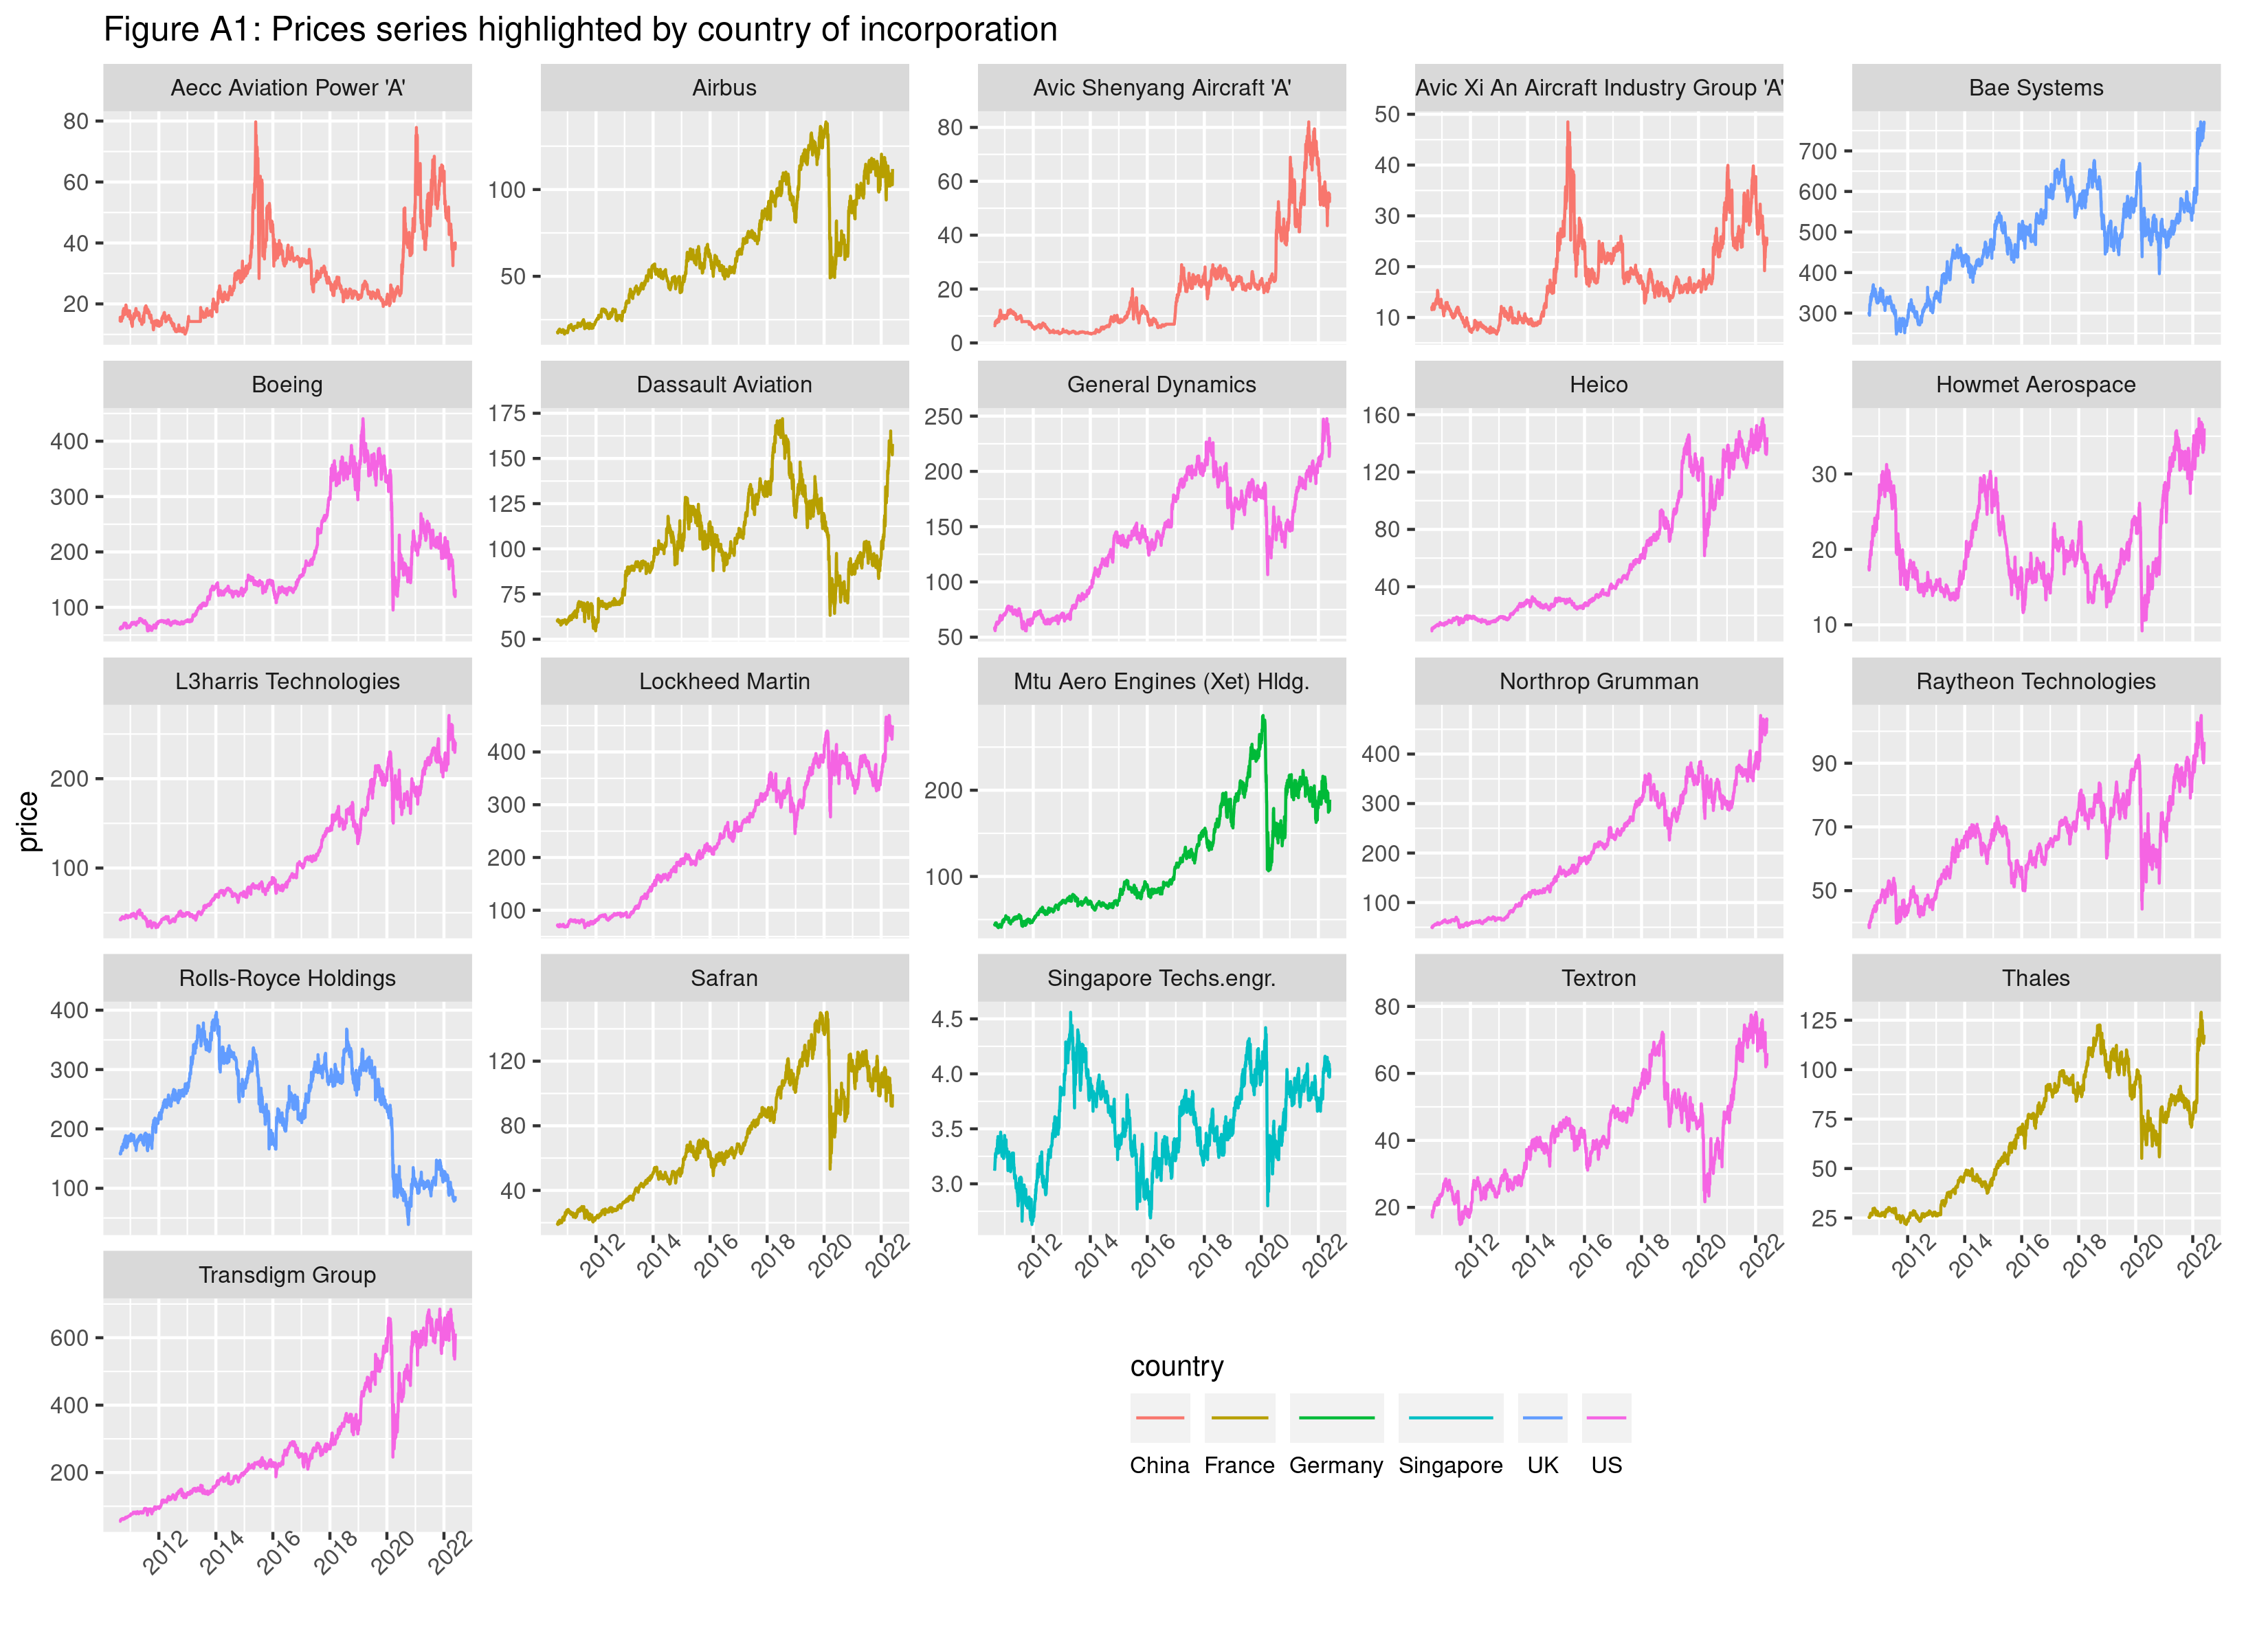
\includegraphics{plots/figA1.png}
\end{sidewaysfigure}

\begin{sidewaysfigure}
\centering
  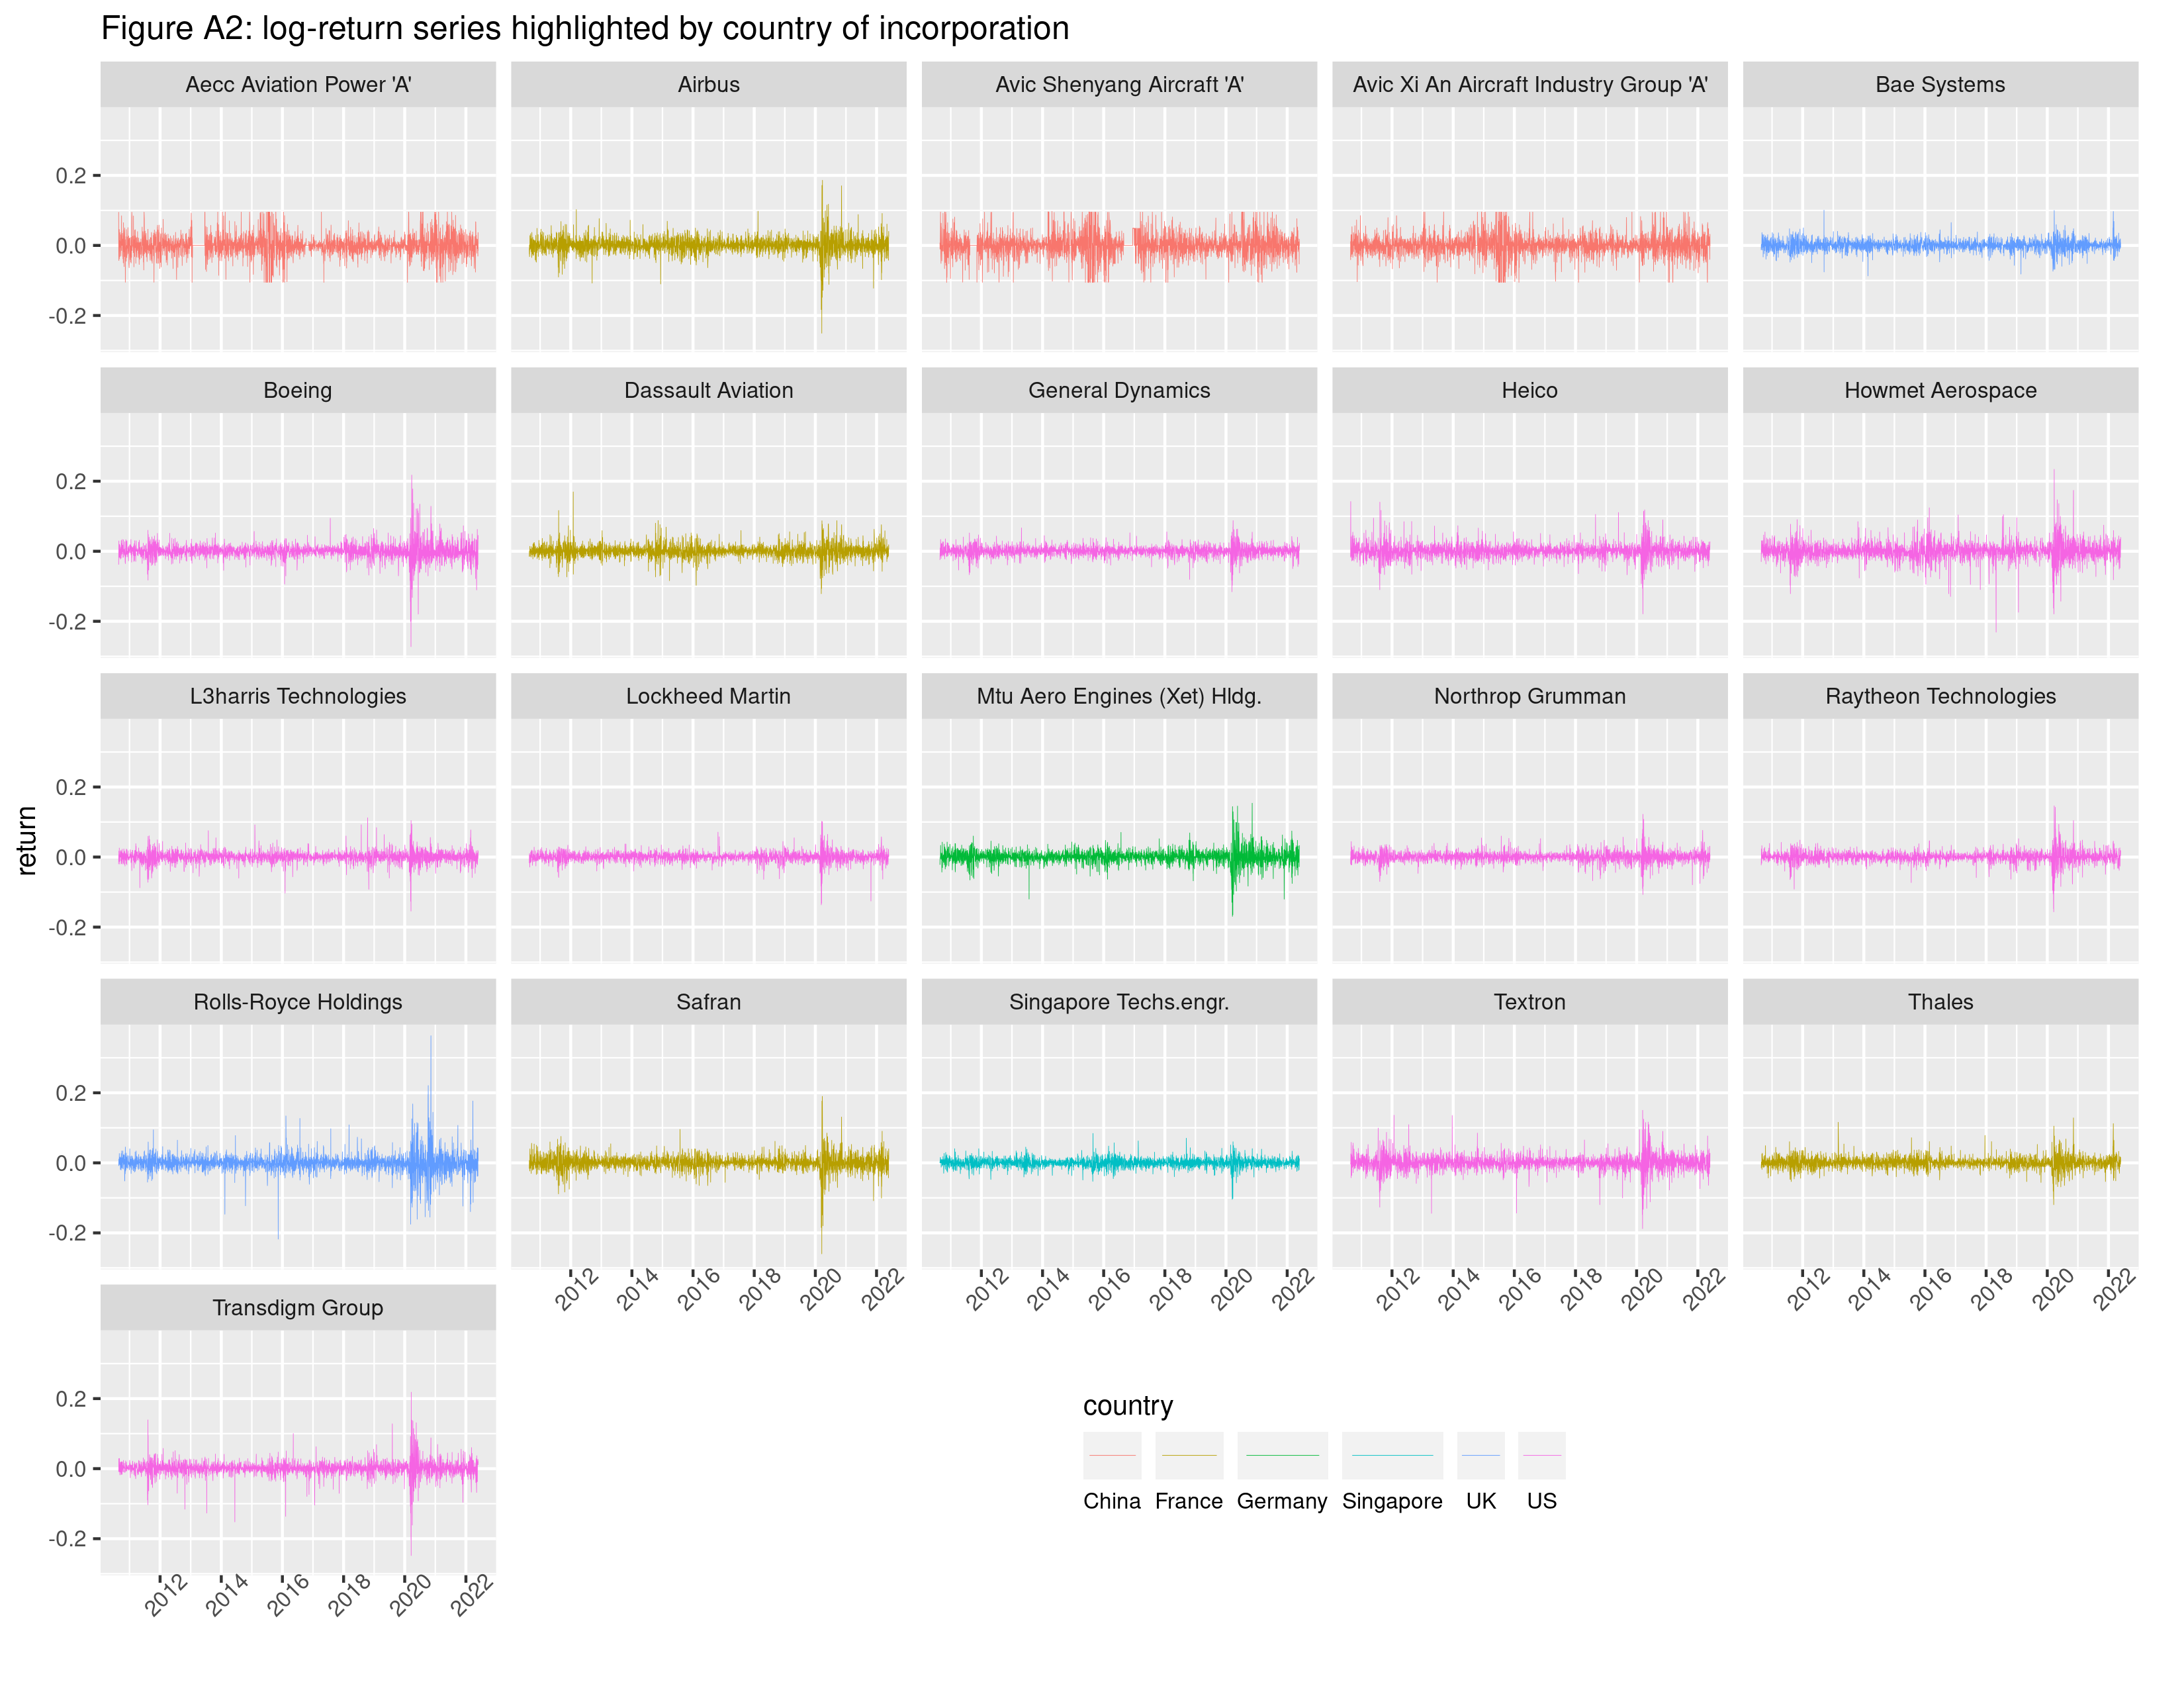
\includegraphics{plots/figA2.png}
\end{sidewaysfigure}

\begin{sidewaysfigure}
\centering
  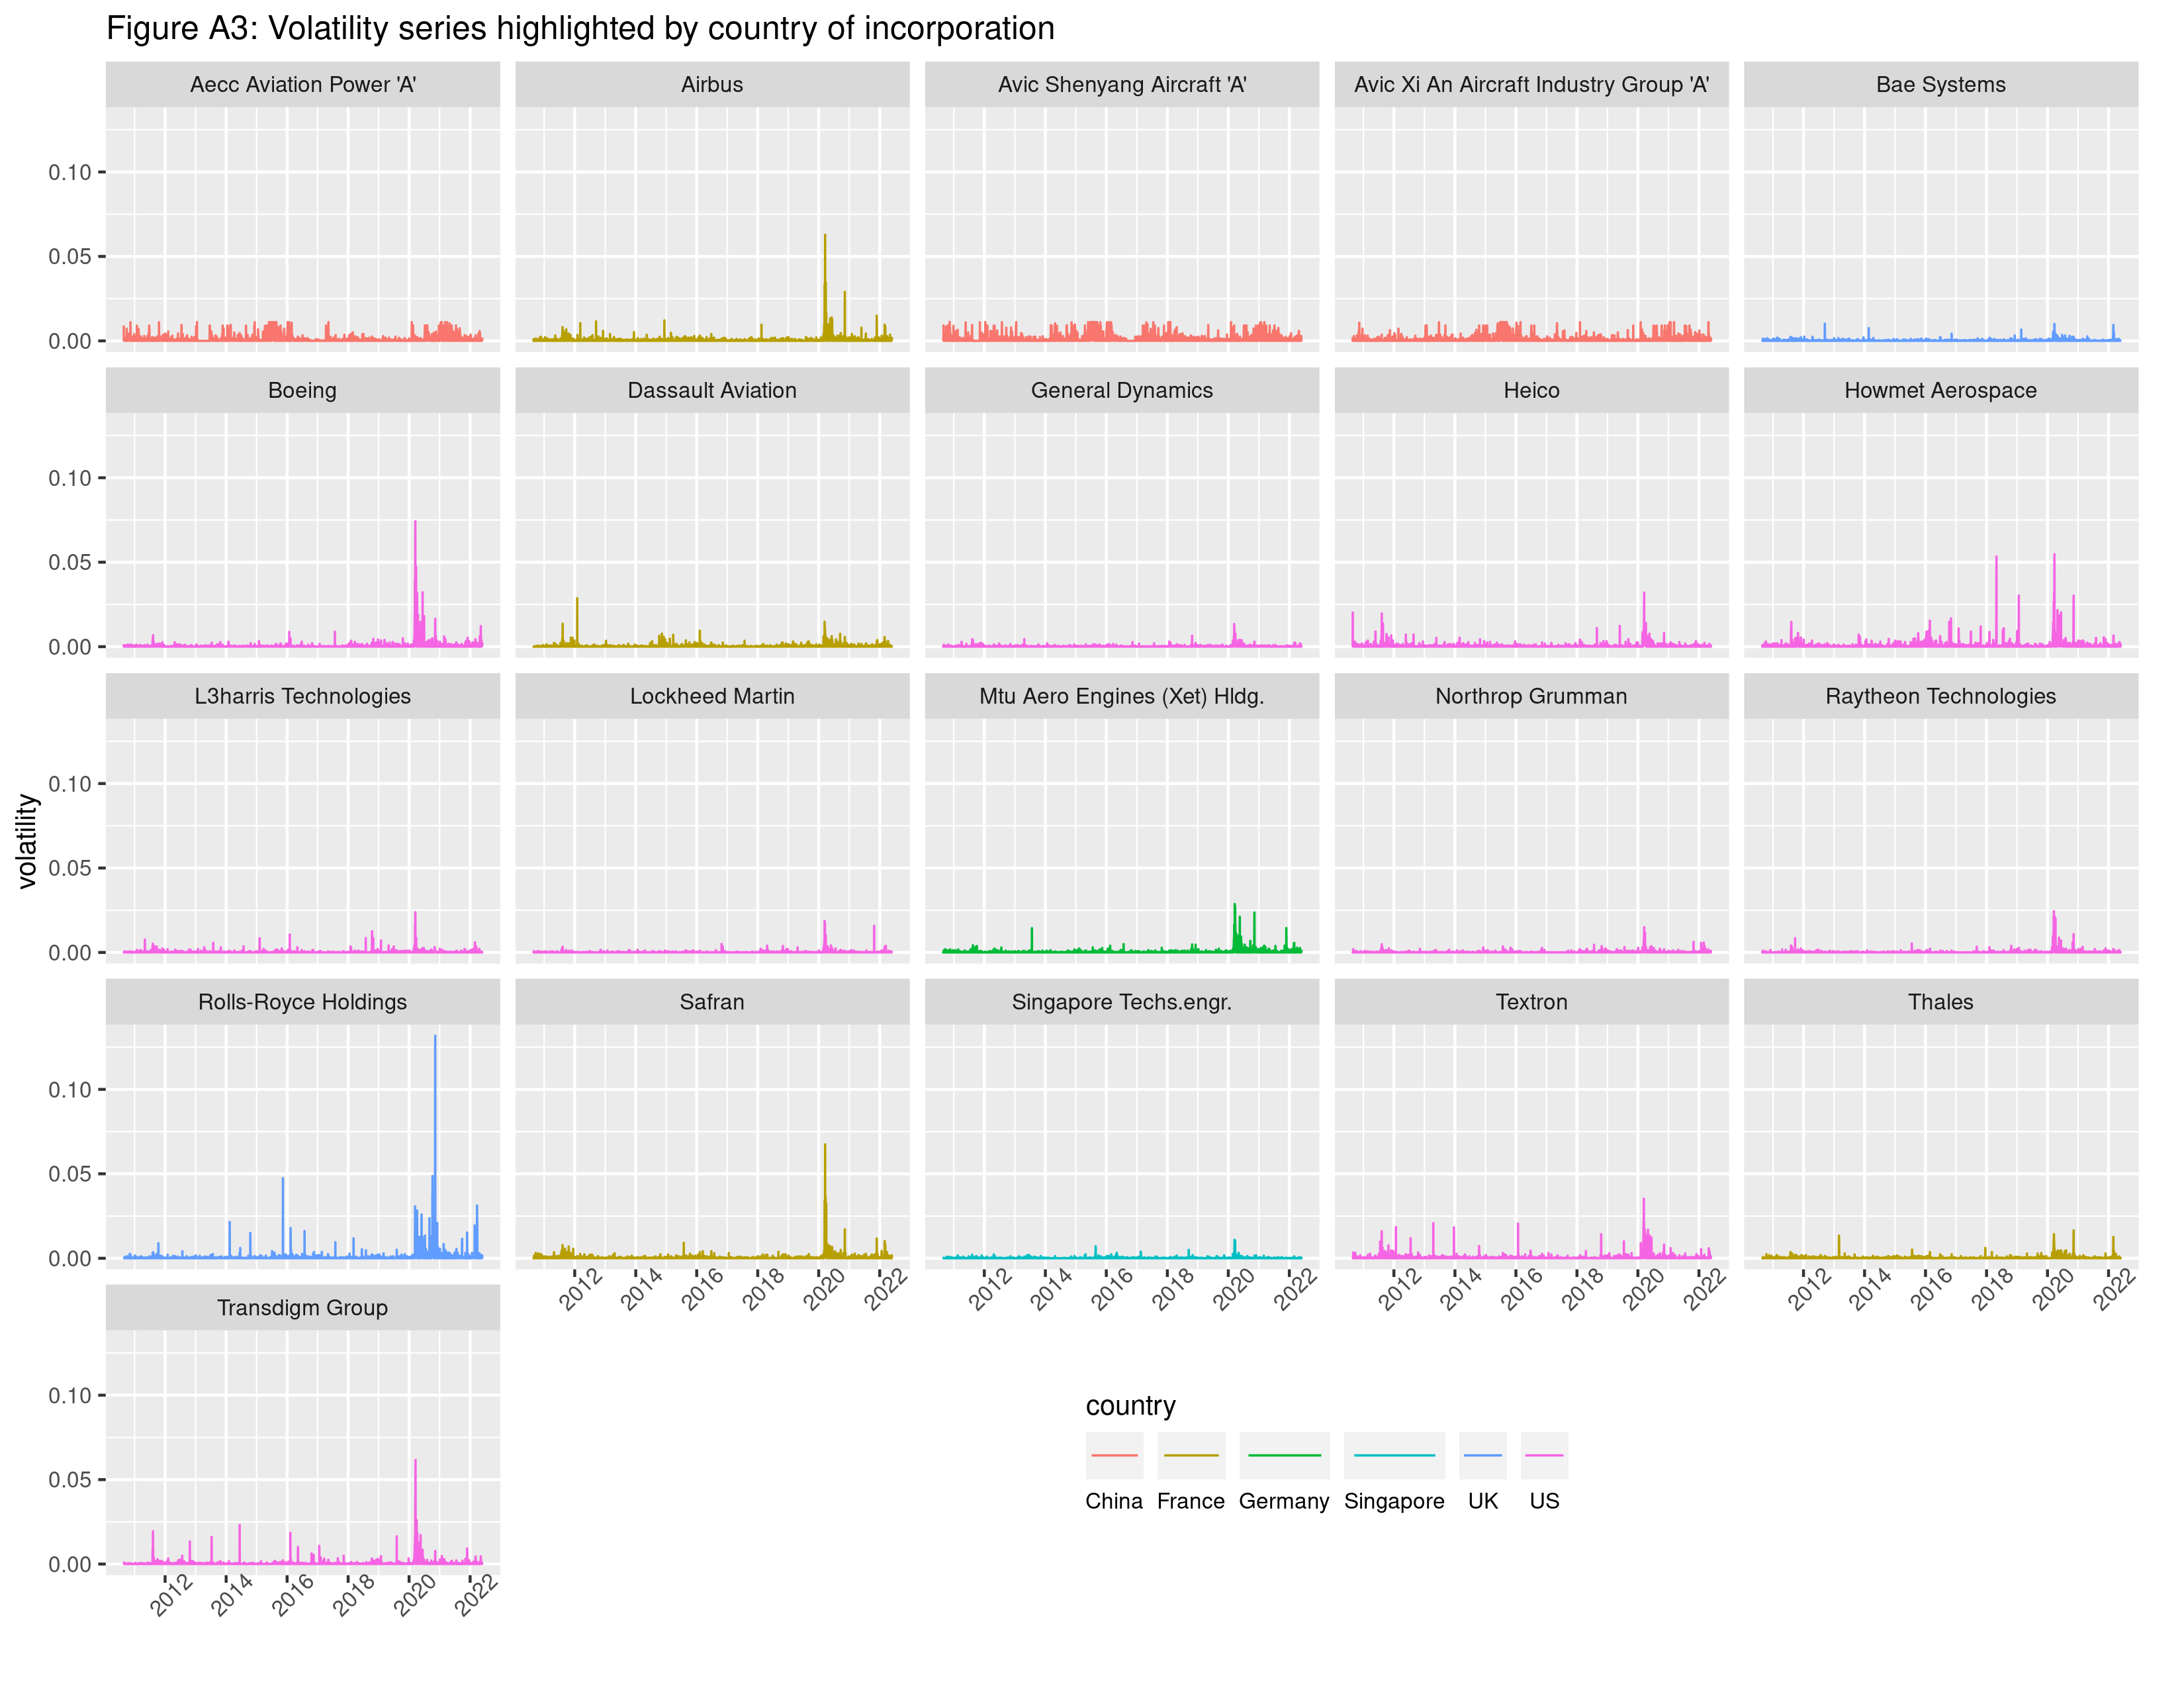
\includegraphics{plots/figA3.png}
\end{sidewaysfigure}

\hypertarget{tbl-A2}{}
\begin{table}[H]
\caption{\label{tbl-A2}Size information for our study's sample }\tabularnewline

\centering
\resizebox{\linewidth}{!}{
\begin{tabular}[t]{lllllllll}
\toprule
A\&D Stock & Mean & Median & Std..Dev. & Skewness & Kurtosis & Jarque.Bera & ADF & PP\\
\midrule
Raytheon Technologies & 0.0003 & 0.0000 & 0.0157 & -0.3658 & 18.8916 & 32636.5*** & -21.2901*** & -56.4338***\\
Lockheed Martin & 0.0006 & 0.0005 & 0.0132 & -0.7847 & 18.2347 & 30248.2*** & -56.5766*** & -56.7477***\\
Boeing & 0.0003 & 0.0000 & 0.0226 & -0.5643 & 26.2666 & 69973.9*** & -18.1156*** & -52.3339***\\
Airbus & 0.0005 & 0.0002 & 0.0222 & -0.3905 & 16.9639 & 25224.5*** & -41.3354*** & -53.1875***\\
Northrop Grumman & 0.0007 & 0.0005 & 0.0142 & -0.1678 & 10.8567 & 7974.9*** & -57.6092*** & -57.9145***\\
\addlinespace
General Dynamics & 0.0004 & 0.0003 & 0.0138 & -0.4154 & 9.2145 & 5069.4*** & -56.0303*** & -56.0601***\\
L3harris Technologies & 0.0006 & 0.0004 & 0.0156 & -0.3236 & 13.3721 & 13927.4*** & -37.8971*** & -58.3311***\\
Safran & 0.0005 & 0.0000 & 0.0208 & -0.5873 & 23.2326 & 52968.0 & -27.1859*** & -54.0423***\\
Transdigm Group & 0.0007 & 0.0006 & 0.0204 & -0.8467 & 26.8661 & 73823.1 & -27.2219*** & -58.6233***\\
Bae Systems & 0.0003 & 0.0000 & 0.0145 & 0.0418 & 7.8111 & 2985.9 & -54.9012*** & -54.8972***\\
\addlinespace
Thales & 0.0005 & 0.0000 & 0.0157 & 0.3395 & 10.4513 & 7219.4 & -52.8929*** & -52.8478***\\
Aecc Aviation Power  A & 0.0004 & 0.0000 & 0.0283 & -0.0139 & 6.3355 & 1434.8 & -50.3413*** & -50.2565***\\
Heico & 0.0009 & 0.0004 & 0.0198 & 0.2280 & 11.1453 & 8582.7 & -37.9681*** & -57.4079***\\
Avic Shenyang Aircraft  A & 0.0007 & 0.0000 & 0.0317 & -0.1037 & 5.3171 & 697.9 & -50.4755*** & -50.432***\\
Textron & 0.0004 & 0.0000 & 0.0215 & -0.3143 & 13.2261 & 13536.4 & -56.7672*** & -56.7572***\\
\addlinespace
Howmet Aerospace & 0.0002 & 0.0000 & 0.0250 & -0.3118 & 13.7557 & 14968.7 & -55.6534*** & -55.6534***\\
Avic Xi An Aircraft Industry Group  A & 0.0003 & 0.0000 & 0.0274 & -0.1139 & 6.1919 & 1320.5 & -51.6737*** & -51.6765***\\
Dassault Aviation & 0.0003 & 0.0000 & 0.0177 & 0.2804 & 10.4996 & 7293.6 & -59.0881*** & -59.3442***\\
Mtu Aero Engines  Xet  Hldg & 0.0004 & 0.0000 & 0.0196 & -0.2349 & 14.6874 & 17643.4 & -53.5665*** & -53.5378***\\
Rolls Royce Holdings & -0.0002 & 0.0000 & 0.0263 & 0.8073 & 25.6142 & 66286.0 & -42.2588*** & -53.3912***\\
\addlinespace
Singapore Techs Engr & 0.0001 & 0.0000 & 0.0121 & -0.2655 & 9.6055 & 5663.1 & -58.7849*** & -58.7819***\\
\bottomrule
\multicolumn{9}{l}{\textsuperscript{} Notes: The sample period is 23 August 2010 – July 1, 2022, yielding 3095 daily return observations. ADF (Augmented Dickey-Fuller) and PP}\\
\multicolumn{9}{l}{(Phillips-Perron) stationarity tests. They are conducted with a constant. The lag length is selected based on SIC. *** indicates statistical}\\
\multicolumn{9}{l}{significance at the 1\% level.}\\
\end{tabular}}
\end{table}

\hypertarget{tbl-A3}{}
\begin{table}[H]
\caption{\label{tbl-A3}Summary statistics of daily volatilies }\tabularnewline

\centering
\resizebox{\linewidth}{!}{
\begin{tabular}[t]{lllllllll}
\toprule
A\&D Stock & Mean & Median & Std..Dev. & Skewness & Kurtosis & Jarque.Bera & ADF & PP\\
\midrule
Raytheon Technologies & 0.0002 & 0.0000 & 0.0010 & 14.3977 & 270.2230 & 9315605 & -8.8644*** & -71.0605***\\
Lockheed Martin & 0.0002 & 0.0000 & 0.0007 & 16.4325 & 350.1678 & 15682053 & -10.8166*** & -57.4850***\\
Boeing & 0.0005 & 0.0001 & 0.0026 & 16.0817 & 339.0628 & 14697726 & -9.4739*** & -59.9743***\\
Airbus & 0.0005 & 0.0001 & 0.0020 & 17.2260 & 424.2219 & 23033869 & -11.5572*** & -65.0529***\\
Northrop Grumman & 0.0002 & 0.0000 & 0.0006 & 11.4526 & 195.7092 & 4856762 & -10.5620*** & -55.0415***\\
\addlinespace
General Dynamics & 0.0002 & 0.0000 & 0.0005 & 10.7424 & 180.7454 & 4133764 & -9.4617*** & -64.1503***\\
L3harris Technologies & 0.0002 & 0.0001 & 0.0009 & 13.5332 & 273.2503 & 9512974 & -11.8003*** & -53.9115***\\
Safran & 0.0004 & 0.0001 & 0.0020 & 19.3285 & 499.2195 & 31946613 & -11.6048*** & -62.0761***\\
Transdigm Group & 0.0004 & 0.0001 & 0.0021 & 16.7444 & 377.0165 & 18184391 & -8.6389*** & -55.6789***\\
Bae Systems & 0.0002 & 0.0001 & 0.0006 & 9.3253 & 129.7845 & 2117775 & -16.0119*** & -50.1728***\\
\addlinespace
Thales & 0.0002 & 0.0001 & 0.0008 & 11.6051 & 190.9520 & 4625049 & -16.3795*** & -60.5916***\\
Aecc Aviation Power  A & 0.0008 & 0.0001 & 0.0018 & 3.8458 & 18.4539 & 38428 & -9.8441*** & -62.2551***\\
Heico & 0.0004 & 0.0001 & 0.0013 & 11.4285 & 201.3856 & 5142764 & -9.5040*** & -65.6277***\\
Avic Shenyang Aircraft  A & 0.0010 & 0.0002 & 0.0021 & 3.2338 & 13.5866 & 19848 & -10.2645*** & -62.4013***\\
Textron & 0.0005 & 0.0001 & 0.0016 & 10.1877 & 141.4459 & 2525317 & -10.6989*** & -55.9341***\\
\addlinespace
Howmet Aerospace & 0.0006 & 0.0001 & 0.0022 & 13.6603 & 265.6162 & 8990159 & -15.2603*** & -62.3260***\\
Avic Xi An Aircraft Industry Group  A & 0.0007 & 0.0002 & 0.0017 & 4.0915 & 21.3110 & 51874 & -10.7828*** & -60.2592***\\
Dassault Aviation & 0.0003 & 0.0001 & 0.0010 & 12.8240 & 286.0500 & 10416628 & -12.8417*** & -55.6529***\\
Mtu Aero Engines  Xet  Hldg & 0.0004 & 0.0001 & 0.0014 & 11.7559 & 179.1791 & 4074035 & -9.3358*** & -66.7664***\\
Rolls Royce Holdings & 0.0007 & 0.0001 & 0.0034 & 21.7076 & 718.3667 & 66237434 & -5.3944*** & -63.2794***\\
\addlinespace
Singapore Techs Engr & 0.0001 & 0.0000 & 0.0004 & 13.5671 & 279.9223 & 9984241 & -12.0964*** & -67.2677***\\
\bottomrule
\multicolumn{9}{l}{\textsuperscript{} Notes: The sample period is 23 August 2010 – July 1, 2022, yielding 3095 daily volatility observations. Volatility is computed as squared}\\
\multicolumn{9}{l}{returns. ADF (Augmented Dickey-Fuller) and PP (Phillips-Perron) stationarity tests. They are conducted with a constant. The lag length is}\\
\multicolumn{9}{l}{selected based on SIC. *** indicates statistical significance at the 1\% level.}\\
\end{tabular}}
\end{table}

\newpage{}

\hypertarget{tbl-A4}{}
\begin{table}[H]
\caption{\label{tbl-A4}Drivers of return spillovers across A\&D companies for the entire sample
period -- Robustness analysis }\tabularnewline

\centering
\resizebox{\linewidth}{!}{
\begin{tabular}[t]{lcccccc}
\toprule
\multicolumn{1}{c}{ } & \multicolumn{2}{c}{Middle Quantile} & \multicolumn{2}{c}{Upper Quantile} & \multicolumn{2}{c}{Lower Quantile} \\
\cmidrule(l{3pt}r{3pt}){2-3} \cmidrule(l{3pt}r{3pt}){4-5} \cmidrule(l{3pt}r{3pt}){6-7}
Variable & Coefficient & Prob. & Coefficient & Prob. & Coefficient & Prob.\\
\midrule
GPRDACT(-1) & -0.024 & 0.000 & -0.001 & 0.006 & -0.003 & 0.000\\
GPRDACT(-1).DCOVID & 0.062 & 0.000 & 0.007 & 0.000 & 0.007 & 0.000\\
USEPU(-1) & 0.011 & 0.000 & 0.001 & 0.004 & 0.001 & 0.018\\
VIX(-1) & 0.233 & 0.000 & 0.017 & 0.005 & 0.032 & 0.000\\
SP500(-1) & 32.246 & 0.005 & 0.716 & 0.604 & 6.999 & 0.000\\
\addlinespace
TERM SPREAD(-1) & -0.674 & 0.831 & 0.538 & 0.207 & -0.473 & 0.287\\
TED SPREAD(-1) & -0.080 & 0.000 & -0.006 & 0.000 & -0.003 & 0.082\\
DEFAULT SPREAD(-1) & 19.778 & 0.000 & 1.393 & 0.000 & 0.698 & 0.000\\
ADS BUS CONDITION INDEX(-1) & 0.770 & 0.000 & 0.077 & 0.000 & 0.071 & 0.000\\
US INFLATION(-1) & 3.485 & 0.000 & 0.205 & 0.006 & -0.423 & 0.000\\
\addlinespace
C & 37.967 & 0.000 & 90.968 & 0.000 & 92.644 & 0.000\\
Adjusted R-squared & 0.610 & NA & 0.373 & NA & 0.383 & NA\\
F-statistic & 412.369 & NA & 157.586 & NA & 164.259 & NA\\
Prob.(F-statistic) & 0.000 & NA & 0.000 & NA & 0.000 & NA\\
\bottomrule
\multicolumn{7}{l}{\textsuperscript{} **Notes**: This table conducts a robustness analysis by replacing the GPR index with the}\\
\multicolumn{7}{l}{GPRACT sub-index in the regression model specified in Equation (6). The sample period is}\\
\multicolumn{7}{l}{23 August 2010 – July 1, 2022.}\\
\end{tabular}}
\end{table}

\hypertarget{tbl-A5}{}
\begin{table}[H]
\caption{\label{tbl-A5}Drivers of volatility spillovers across A\&D companies for the entire
sample period -- Robustness analysis }\tabularnewline

\centering
\resizebox{\linewidth}{!}{
\begin{tabular}[t]{lcccccc}
\toprule
\multicolumn{1}{c}{ } & \multicolumn{2}{c}{Middle Quantile} & \multicolumn{2}{c}{Upper Quantile} & \multicolumn{2}{c}{Lower Quantile} \\
\cmidrule(l{3pt}r{3pt}){2-3} \cmidrule(l{3pt}r{3pt}){4-5} \cmidrule(l{3pt}r{3pt}){6-7}
Variable & Coefficient & Prob. & Coefficient & Prob. & Coefficient & Prob.\\
\midrule
GPRD(-1) & -0.033 & 0.000 & -0.001 & 0.059 & -0.015 & 0.002\\
GPRD(-1).DCOVID & 0.101 & 0.000 & 0.001 & 0.485 & 0.058 & 0.000\\
USEPU(-1) & 0.041 & 0.000 & 0.000 & 0.173 & 0.019 & 0.000\\
VIX(-1) & 0.624 & 0.000 & 0.001 & 0.883 & 0.507 & 0.000\\
SP500(-1) & 98.243 & 0.000 & -0.925 & 0.489 & 70.371 & 0.000\\
\addlinespace
TERM SPREAD(-1) & -6.741 & 0.248 & -1.232 & 0.004 & -6.009 & 0.134\\
TED SPREAD(-1) & -0.031 & 0.302 & 0.000 & 0.821 & -0.069 & 0.001\\
CORPORATE CREDIT CONDITIONS(-1) & 13.995 & 0.000 & 0.070 & 0.636 & 16.155 & 0.000\\
ADS BUS CONDITION INDEX(-1) & 1.105 & 0.000 & 0.002 & 0.784 & 0.759 & 0.000\\
US INFLATION(-1) & 5.182 & 0.000 & -0.025 & 0.692 & 6.020 & 0.000\\
\addlinespace
C & 15.912 & 0.000 & 94.856 & 0.000 & 27.367 & 0.000\\
Adjusted R-squared & 0.551 & NA & 0.011 & NA & 0.580 & NA\\
F-statistic & 323.154 & NA & 3.900 & NA & 363.583 & NA\\
Prob.(F-statistic) & 0.000 & NA & 0.000 & NA & 0.000 & NA\\
\bottomrule
\multicolumn{7}{l}{\textsuperscript{} **Notes**: This table conducts a robustness analysis by replacing the GPR index with the}\\
\multicolumn{7}{l}{GPRACT sub-index in the regression model specified in Equation (6). The sample period is 23}\\
\multicolumn{7}{l}{August 2010 – July 1, 2022.}\\
\end{tabular}}
\end{table}

\newpage{}

\hypertarget{references}{%
\section*{References}\label{references}}
\addcontentsline{toc}{section}{References}

\hypertarget{refs}{}
\begin{CSLReferences}{1}{0}
\leavevmode\vadjust pre{\hypertarget{ref-agapos1970}{}}%
Agapos, A. M., and L. E. Gallaway. 1970. {``Defence Profits and the
Renegotiation Board in the Aerospace Industry.''} \emph{Journal of
Political Economy} 78 (5): 1093--1105.
\url{https://doi.org/10.1086/259692}.

\leavevmode\vadjust pre{\hypertarget{ref-alqahtani2020}{}}%
Alqahtani, A., E. Bouri, and X. V. Vo. 2020. {``Predictability of GCC
Stock Returns: The Role of Geopolitical Risk and Crude Oil Returns.''}
\emph{Economic Analysis and Policy} 68: 239--49.
\url{https://doi.org/10.1016/j.eap.2020.09.017}.

\leavevmode\vadjust pre{\hypertarget{ref-ando2022}{}}%
Ando, T., M. Greenwood-Nimmo, and Y. Shin. 2022. {``Quantile
Connectedness: Modeling Tail Behavior in the Topology of Financial
Networks.''} \emph{Management Science} 68 (4): 2401--31.
\url{https://doi.org/10.1287/mnsc.2021.3984}.

\leavevmode\vadjust pre{\hypertarget{ref-Ando.2022}{}}%
Ando, Tomohiro, Matthew Greenwood-Nimmo, and Yongcheol Shin. 2022.
{``{Quantile Connectedness: Modeling Tail Behavior in the Topology of
Financial Networks}.''} \emph{Management Science} 68 (4): 2401--31.
\url{https://doi.org/10.1287/mnsc.2021.3984}.

\leavevmode\vadjust pre{\hypertarget{ref-apergis2017}{}}%
Apergis, Nicholas, Matteo Bonato, Rangan Gupta, and Clement Kyei. 2017.
{``Does Geopolitical Risks Predict Stock Returns and Volatility of
Leading Defense Companies? Evidence from a Nonparametric Approach.''}
\emph{Defence and Peace Economics}, February, 1--13.
\url{https://doi.org/10.1080/10242694.2017.1292097}.

\leavevmode\vadjust pre{\hypertarget{ref-aruoba2009}{}}%
Aruoba, S. B., F. X. Diebold, and C. Scotti. 2009. {``Real-Time
Measurement of Business Conditions.''} \emph{Journal of Business \&
Economic Statistics} 27 (4): 417--27.
\url{https://doi.org/10.1198/jbes.2009.07205}.

\leavevmode\vadjust pre{\hypertarget{ref-baker2016}{}}%
Baker, S. R., N. Bloom, and S. J. Davis. 2016. {``Measuring Economic
Policy Uncertainty.''} \emph{The Quarterly Journal of Economics} 131
(4): 1593--1636. \url{https://doi.org/10.1093/qje/qjw024}.

\leavevmode\vadjust pre{\hypertarget{ref-NYfed.2022}{}}%
Barone, Jordan, Alain Chaboud, Adam Copeland, Cullen Kavoussi, Frank M.
Keane, and Searls, and Seth. 2022. {``{The Global Dash for Cash: Why
Sovereign Bond Market Functioning Varied across Jurisdictions in March
2020}.''} \emph{New York Federal Reserve Bank Staff Report}, March.
\url{https://www.newyorkfed.org/research/staff/_reports/sr1010}.

\leavevmode\vadjust pre{\hypertarget{ref-bohi1973}{}}%
Bohi, D. R. 1973. {``Profit Performance in the Defence Industry.''}
\emph{Journal of Political Economy} 81 (3): 721--28.
\url{https://doi.org/10.1086/260067}.

\leavevmode\vadjust pre{\hypertarget{ref-Bouri.2020}{}}%
Bouri, E., B. Lucey, T. Saeed, and X. V. Vo. 2020a. {``Extreme
Spillovers Across Asian-Pacific Currencies: A Quantile-Based
Analysis.''} \emph{International Review of Financial Analysis} 72:
101605.
https://doi.org/\url{https://doi.org/10.1016/j.irfa.2020.101605}.

\leavevmode\vadjust pre{\hypertarget{ref-bouri2020}{}}%
---------. 2020b. {``Extreme Spillovers Across Asian-Pacific Currencies:
A Quantile-Based Analysis.''} \emph{International Review of Financial
Analysis} 72: 101605. \url{https://doi.org/10.1016/j.irfa.2020.101605}.

\leavevmode\vadjust pre{\hypertarget{ref-bouwer2022}{}}%
Bouwer, J., V. Krishnan, S. Saxon, and C. Tufft. 2022. {``Taking Stock
of the Pandemic's Impact on Global Aviation.''} 2022.
\url{https://www.mckinsey.com/industries/travel-logistics-and-infrastructure/our-insights/taking-stock-of-the-pandemics-impact-on-global-aviation}.

\leavevmode\vadjust pre{\hypertarget{ref-bu2019}{}}%
Bu, H., W. Tang, and J. Wu. 2019. {``Time-Varying Comovement and Changes
of Comovement Structure in the Chinese Stock Market: A Causal Network
Method.''} \emph{Economic Modelling} 81: 181--204.
\url{https://doi.org/10.1016/j.econmod.2019.03.002}.

\leavevmode\vadjust pre{\hypertarget{ref-butler1966}{}}%
Butler, Hartman L. 1966. {``Aerospace Fundamentals and Industry
Analysis: Part II.''} \emph{Financial Analysts Journal} 22 (2): 41--48.
\url{https://doi.org/10.2469/faj.v22.n2.41}.

\leavevmode\vadjust pre{\hypertarget{ref-butler1967}{}}%
---------. 1967. {``Aerospace Industry Revisited.''} \emph{Financial
Analysts Journal} 23 (5): 57--62.
\url{https://doi.org/10.2469/faj.v23.n5.57}.

\leavevmode\vadjust pre{\hypertarget{ref-butler1966a}{}}%
Butler Jr, H. L. 1966a. {``Aerospace Fundamentals and Industry Analysis:
Part i.''} \emph{Financial Analysts Journal} 22 (1): 55--60.
\url{https://doi.org/10.2469/faj.v22.n1.55}.

\leavevmode\vadjust pre{\hypertarget{ref-butler1966b}{}}%
---------. 1966b. {``Aerospace Fundamentals and Industry Analysis: Part
II.''} \emph{Financial Analysts Journal} 22 (2): 57--62.
\url{https://doi.org/10.2469/faj.v22.n2.57}.

\leavevmode\vadjust pre{\hypertarget{ref-butler1966c}{}}%
---------. 1966c. {``Aerospace Fundamentals and Industry Analysis: Part
III.''} \emph{Financial Analysts Journal} 22 (3): 75--80.
\url{https://doi.org/10.2469/faj.v22.n3.75}.

\leavevmode\vadjust pre{\hypertarget{ref-butler1966d}{}}%
---------. 1966d. {``Aerospace Fundamentals and Industry Analysis: Part
IV.''} \emph{Financial Analysts Journal} 22 (4): 59--64.
\url{https://doi.org/10.2469/faj.v22.n4.59}.

\leavevmode\vadjust pre{\hypertarget{ref-caldara2022measuring}{}}%
Caldara, Dario, and Matteo Iacoviello. 2022. {``Measuring Geopolitical
Risk.''} \emph{American Economic Review} 112 (4): 1194--1225.
\url{https://doi.org/10.1257/aer.20191823}.

\leavevmode\vadjust pre{\hypertarget{ref-Cappelle.2008}{}}%
Capelle‐Blancard, Gunther, and Nicolas Couderc. 2008. {``{What drives
the market value of firms in the defense industry?}''} \emph{Review of
Financial Economics} 17 (1): 14--32.
\url{https://doi.org/10.1016/j.rfe.2007.02.001}.

\leavevmode\vadjust pre{\hypertarget{ref-Diebold.2009}{}}%
Diebold, Francis X., and Kamil Yilmaz. 2009. {``{Measuring Financial
Asset Return and Volatility Spillovers, with Application to Global
Equity Markets*}.''} \emph{The Economic Journal} 119 (534): 158--71.
\url{https://doi.org/10.1111/j.1468-0297.2008.02208.x}.

\leavevmode\vadjust pre{\hypertarget{ref-Diebold.2014}{}}%
Diebold, Francis X., and Kamil Yılmaz. 2014. {``{On the network topology
of variance decompositions: Measuring the connectedness of financial
firms}.''} \emph{Journal of Econometrics} 182 (1): 119--34.
\url{https://doi.org/10.1016/j.jeconom.2014.04.012}.

\leavevmode\vadjust pre{\hypertarget{ref-Dungey.2019}{}}%
Dungey, Mardi, John Harvey, and Vladimir Volkov. 2019. {``{The changing
international network of sovereign debt and financial institutions}.''}
\emph{Journal of International Financial Markets, Institutions and
Money} 60: 149--68. \url{https://doi.org/10.1016/j.intfin.2018.12.013}.

\leavevmode\vadjust pre{\hypertarget{ref-federle2022}{}}%
Federle, Jonathan, and Victor Sehn. 2022. {``Costs of Proximity to War
Zones: Stock Market Responses to the Russian Invasion of Ukraine.''}
\emph{SSRN Electronic Journal}.
\url{https://doi.org/10.2139/ssrn.4060222}.

\leavevmode\vadjust pre{\hypertarget{ref-huang2021}{}}%
Huang, Chuangxia, Yunke Deng, Xiaoguang Yang, Jinde Cao, and Xin Yang.
2021. {``A Network Perspective of Comovement and Structural Change:
Evidence from the Chinese Stock Market.''} \emph{International Review of
Financial Analysis} 76 (July): 101782.
\url{https://doi.org/10.1016/j.irfa.2021.101782}.

\leavevmode\vadjust pre{\hypertarget{ref-kumar2022}{}}%
Kumar, Ashish, Najaf Iqbal, Subrata Kumar Mitra, Ladislav Kristoufek,
and Elie Bouri. 2022. {``Connectedness Among Major Cryptocurrencies in
Standard Times and During the COVID-19 Outbreak.''} \emph{Journal of
International Financial Markets, Institutions and Money} 77 (March):
101523. \url{https://doi.org/10.1016/j.intfin.2022.101523}.

\leavevmode\vadjust pre{\hypertarget{ref-le2022}{}}%
Le, Viet Hoang, Hans-Jörg von Mettenheim, Stéphane Goutte, and Fei Liu.
2022. {``News-Based Sentiment: Can It Explain Market Performance Before
and After the Russia{\textendash}Ukraine~Conflict?''} \emph{The Journal
of Risk Finance} 24 (1): 72--88.
\url{https://doi.org/10.1108/jrf-06-2022-0168}.

\leavevmode\vadjust pre{\hypertarget{ref-Londono.2019}{}}%
Londono, Juan M. 2019. {``{Bad bad contagion}.''} \emph{Journal of
Banking \& Finance} 108: 105652.
\url{https://doi.org/10.1016/j.jbankfin.2019.105652}.

\leavevmode\vadjust pre{\hypertarget{ref-mcdonald2011}{}}%
McDonald, James E., and Walter R. Kendall. 2011. {``Measuring the
Economic Effects of Political Events: War and the u.s. Defense
Industry.''} \emph{Journal of Applied Business Research (JABR)} 10 (1):
57. \url{https://doi.org/10.19030/jabr.v10i1.5963}.

\leavevmode\vadjust pre{\hypertarget{ref-neely2022}{}}%
Neely, Christopher J. 2022. {``Financial Market Reactions to the Russian
Invasion of Ukraine.''} \url{https://doi.org/10.20955/wp.2022.032}.

\leavevmode\vadjust pre{\hypertarget{ref-reichardt}{}}%
Reichardt, Kelly. n.d. {``An Interview with Kelly Reichardt.''} In,
111--24. University of Illinois Press.
\url{https://doi.org/10.5406/j.ctt1xhr4wz.5}.

\leavevmode\vadjust pre{\hypertarget{ref-sillars2021}{}}%
Sillars, J. 2021. {``COVID-19: Rolls-Royce Blames {`Severe Impact'} of
Pandemic as It Dives to £4bn Loss.''} Sky News. 2021.
\url{https://news.sky.com/story/covid-19-rolls-royce-blames-severe-impact-of-pandemic-as-it-dives-to-4bn-loss-12242499}.

\leavevmode\vadjust pre{\hypertarget{ref-suarez1976}{}}%
Suarez, James M. 1976. {``Profits and Performance of Aerospace Defense
Contractors.''} \emph{Journal of Economic Issues} 10 (2): 386--402.
\url{https://doi.org/10.1080/00213624.1976.11503352}.

\leavevmode\vadjust pre{\hypertarget{ref-valukonis2014}{}}%
Valukonis, Mantas. 2014. {``CHINA's STOCK MARKET TRENDS AND THEIR
DETERMINANTS ANALYSIS USING MARKET INDICES.''} \emph{ECONOMICS AND
MANAGEMENT} 18 (4). \url{https://doi.org/10.5755/j01.em.18.4.5096}.

\leavevmode\vadjust pre{\hypertarget{ref-zhang2022}{}}%
Zhang, Zhengyong, Elie Bouri, Tony Klein, and Naji Jalkh. 2022.
{``Geopolitical Risk and the Returns and Volatility of Global Defense
Companies: A New Race to Arms?''} \emph{International Review of
Financial Analysis} 83 (October): 102327.
\url{https://doi.org/10.1016/j.irfa.2022.102327}.

\end{CSLReferences}



\end{document}
